\documentclass[a4paper,11pt]{report}
\usepackage[utf8]{inputenc}
\usepackage{graphicx}
\graphicspath{ {images/} } %where images live

\usepackage{amssymb}	%for extended maths input
\usepackage{multirow,array}	%for payoff matrices
\usepackage{tikz}	%for graphics
\usetikzlibrary{graphs,graphs.standard}	%tikz package for graphs
\usepackage{amsmath, graphics, setspace} %for mathematica images
\usepackage{subcaption} %for side-by-side figures
\usepackage{hyperref}
\usepackage{url}

\usepackage{csvsimple}

%%make it pretty (headers)
%\usepackage{fancyhdr}
%\pagestyle{fancy}
%\fancyhead[LO]{\sffamily\itshape \thesubsection \thesubsection}

\usepackage{cite}

% for lists
\usepackage{enumitem}

%for multi-level lists
\newlist{inparaenum}{enumerate}{2}% allow two levels of nesting in an enumerate-like environment
\setlist[inparaenum]{nosep}% compact spacing for all nesting levels
\setlist[inparaenum,1]{label=\alph*.}% labels for top level
\setlist[inparaenum,2]{label=\alph{inparaenumi}\alph*)}% labels for second level



\usepackage{mathtools}
\DeclarePairedDelimiter{\abs}{\lvert}{\rvert}
\DeclarePairedDelimiter{\norm}{\lVert}{\rVert}

\newcommand\tab[1][0.4cm]{\hspace*{#1}} %add tab function

%including code
\usepackage{color}
\usepackage{listings}

\definecolor{codegreen}{rgb}{0.2,0.1,0}
\definecolor{codegray}{rgb}{0.5,0.5,0.5}
\definecolor{codepurple}{rgb}{0.58,0,0.4}
\definecolor{backcolour}{rgb}{0.95,0.95,0.92}

\lstdefinestyle{mystyle}{
	backgroundcolor=\color{backcolour},   
	commentstyle=\color{codegreen},
	keywordstyle=\color{codepurple},
	numberstyle=\tiny\color{codegray},
	stringstyle=\color{codepurple},
	basicstyle=\footnotesize,
	breakatwhitespace=false,         
	breaklines=true,                 
	captionpos=b,                    
	keepspaces=true,                 
	numbers=left,                    
	numbersep=5pt,                  
	showspaces=false,                
	showstringspaces=false,
	showtabs=false,                  
	tabsize=2
}

\lstset{style=mystyle}


%%making the 'lessons' coloured section
%
\usepackage[most]{tcolorbox}
\usepackage{xcolor}

\definecolor{susceptible-colour}{HTML}{F2728C}
\definecolor{exposed-colour}{HTML}{67B8C7}
\definecolor{infective-colour}{HTML}{F2728C}
\definecolor{removed-colour}{HTML}{67B8C7}
%Susceptible, green, #ADD694
%Exposed, yellow, #FFCD47
%Infected, pink, #F2728C
%Recovered, blue, #67B8C7

\tcbset{
	frame code={}
	center title,
	left=0pt,
	right=0pt,
	top=0pt,
	bottom=0pt,
	colback=infective-colour!40,
	colframe=white,
	width=\dimexpr\textwidth\relax,
	enlarge left by=0mm,
	boxsep=5pt,
	arc=0pt,outer arc=0pt,
}

%to have the boltzmann wealth model rules list resume after being seperated by another list
\newcounter{rule}

\newcommand{\reporttitle}{An epidemiological approach to modelling revolution and repression}
\newcommand{\reportauthor}{Joe Kroese}
\newcommand{\studentID}{8386741}
\newcommand{\supervisor}{Dr Mark Muldoon}
\newcommand{\degreetype}{Mathematics}


\begin{document}

\author{Joe Kroese}
\title{An epidemiological approach to modelling revolution and repression}
\date{\today}

%\frontmatter
% Last modification: 2015-08-17 (Marc Deisenroth)
\begin{titlepage}

\newcommand{\HRule}{\rule{\linewidth}{0.5mm}} % Defines a new command for the horizontal lines, change thickness here


%----------------------------------------------------------------------------------------
%	LOGO SECTION
%----------------------------------------------------------------------------------------


\includegraphics[width = 4cm]{TeX_files/figures/imperial.jpg}\\[0.5cm] 

\center % Center remainder of the page

%----------------------------------------------------------------------------------------
%	HEADING SECTIONS
%----------------------------------------------------------------------------------------

\textsc{\Large University of Manchester}\\[0.5cm] 
\textsc{\large School of Mathematics}\\[0.5cm] 

%----------------------------------------------------------------------------------------
%	TITLE SECTION
%----------------------------------------------------------------------------------------

\HRule \\[0.4cm]
{ \huge \bfseries \reporttitle}\\ % Title of your document
\HRule \\[1.5cm]
 
%----------------------------------------------------------------------------------------
%	AUTHOR SECTION
%----------------------------------------------------------------------------------------

\begin{minipage}[t]{0.4\textwidth}
\begin{flushleft} \large
\emph{Author:}\\
\reportauthor \\% Your name
\bigskip
\emph{Student ID:}\\
\studentID
\end{flushleft}
\end{minipage}
~
\begin{minipage}[t]{0.4\textwidth}
\begin{flushright} \large
\emph{Supervisor:} \\
\supervisor % Supervisor's Name
\end{flushright}
\end{minipage}\\[4cm]


%----------------------------------------------------------------------------------------
%	FOOTER & DATE SECTION
%----------------------------------------------------------------------------------------
\vfill % Fill the rest of the page with whitespace
Submitted in fulfillment of the requirements of MATH40000 for the MMath degree in
\degreetype~at the University of Manchester\\[0.5cm]

\makeatletter
\@date 
\makeatother


\end{titlepage}

%\maketitle
\tableofcontents

%\begin{tcolorbox}[colback=susceptible-colour!50,coltext=white]
	\chapter{Introduction}
%\textit{An introduction, giving an overview of the project and its context, and perhaps mentioning prerequisites (such as saying, "the reader should be familiar with a first course in linear Algebra"). Often an introduction will contain a paragraph or so describing briefly what is done in each chapter. It is also worth stressing the original contributions that you have made in the abstract.}\\
%\\
\subsection{Revolution as infectious disease}
%\end{tcolorbox}
%\paragraph{Revolutions are like infectious diseases}
In many ways a revolution is like an infectious disease. Though the mechanics of transmission are inherently different, there are notable parallels. At the centre of a revolution is an idea. This idea spreads through the population by `contact' between individuals. It has hosts, ways of spreading, an origin, hotspots and occasional eruptive dynamics.\\
\\
%\paragraph{Ideas are like infectious diseases}
Research has shown that ideas replicate very similarly to infectious diseases\cite{meme-epidemic}\cite{the-power-of-a-good-idea}. This insight has allowed researchers access to a rich set of methods and vocabulary from mathematical epidemiology to study the spread of ideas through a population. Making simple reinterpretations such as viewing `infectious' as `actively sharing an idea' we can sometimes even use identical models\cite{thomas-house}.\\
\\
%\paragraph{Revolutions have ideas at their core...}
Revolutions are infinitely varied but one common feature is that they all fundamentally rely on ideas. At each revolution's core is some self-replicating idea\footnote{In this way the spreading idea is a `meme' in Richard Dawkins' sense of `a cultural entity that appears to exhibit self-replication'\cite{selfish-gene}.} that inspires and justifies political change. Without this shared idea to rally around the citizens struggle for cohesion making a successful revolution unlikely\cite{tyranny}\cite{logic-non-violence}. If a revolution may be thought of as the revolutionary idea that drives it, we can model the revolution through the spread of the idea.
%As a revolutionary idea is still an idea, a revolution can be modelled as if it were an infectious disease.
\\
\\
%\paragraph{... But they are different}
However, a revolutionary idea is an idea of a special kind in that it carries a risk to those who actively disseminate it. The reason for not sharing most ideas is simply apathy. Meanwhile, a reason to avoid sharing a political idea is fear of imprisonment, social isolation and worse.
%So there is an extra disincentive not to share the revolutionary idea as doing so risks negative personal repercussions from the authorities.
Therefore, whilst we may take inspiration from mathematical epidemiology and research on the spread of ideas, we should do so with caution. In particular we must remember that we will need to add specific extensions to the models that will have no epidemic equivalent.
%\\

%paragraph{Mathematical Epidemiology}
%Epidemiology is the study of how communicable diseases spread between individuals in a population. Mathematics has offered insights into this phenomena since Daniel Bernoulli's paper on inoculation against smallpox in 1760\cite{bernoulli}. Mathematical models have increasingly become a major feature of public health organisation's attempt to eradicate and reduce the spread of diseases. Its clear benefit to medicine has meant that it has quickly developed a rich set of techniques and models.

\subsection{What we talk about when we talk about revolutions}
`Revolution' is an expansive concept. In its most general political and sociological sense a revolution is an effort to transform the political institutions and the justifications for political authority in society by a popular movement in an irregular, extraconstitutional or violent fashion\cite{goldstone_2001}\cite{goodwin-2006}.
This includes events as disparate as the peaceful Philippine Revolution of 1986, the French Revolution and the Egyptian coup d'\'etat of 1952.\\
\\
This paper will look exclusively at `bottom-up' revolutions in which non-violent action played a substantial role. These requirements allow us to focus on the spread of ideas and avoid considerations such as militaristic power which complicate the dynamics. Further there have been recent advances in the statistical analysis of non-violent resistance which provide useful data for analysing and tunings the models. In particular, Erica Chenoweth's \textit{Why Civil Resistance Works: The Strategic Logic of Nonviolent Conflict} has provided a firm footing for the quantitative study of nonviolent revolutions\cite{logic-non-violence}.\\
\\
In particular, our prototypical case will be the Tunisian Revolution in 2010 that marked the beginning of the Arab Spring. The revolution resulted in the overthrow of President Ben Ali after widespread civil resistance in reaction to high levels of unemployment, corruption and restricted press freedom\cite{andrew-gee_2018}. This is often spoken of as the `first digital revolution' due to the significant role social media played in affecting the spread of information, ideas and revolutionary action\cite{social-networks-tunisia}.\\
\\
Previous explanatory models of revolutionary behaviour have focused on spatial processes which undoubtedly play a key role during the peak of a revolution and also throughout pre-digital revolutions\cite{epstein}. However there is a lack of quantitative research into how a revolutionary idea spreads through a society in a way that is general enough to account for the globalising effect of social media. This paper aims to provide a direction for such models, explaining the dynamics of non-violent revolution in a way that can account for all manner of social contact.
%This paper aims to provide a direction for future explanatory models to explain the dynamics of non-violent revolution that is general enough to account for the rapid and globalised communication and organisation that social media facilitates.

\subsection{Paper structure}
%\paragraph{Purpose of paper}
In particular we will develop two models that make no assumptions about the way ideas are transferred, allowing them to be general enough to account for social media communication as well as conventional media. These models will explore two different ways of taking inspiration from mathematical epidemiology to develop original models of political revolution. We will see that the first model, whilst simple, can offer interesting insights whilst being analytically tractable. However the limitations of this model motivate the development of a more complex model that can only be understood statistically but can provide more accurate descriptions.\\
\\
%\paragraph{Compartmental models}
Chapter \ref{ch:compartments} will explore the application of compartmental models to the study of revolutions. We will start by analysing a special case of the Kermack-McKendrick epidemic model known as the SIR model. This will give us a system  of differential equations that we can solve analytically. We will extend this simplistic model by adding some specific nuances to develop a model of the spread of revolutionary ideas. We will also develop some measures to help us build a deeper understanding of the model and, more generally, revolutions.\\
%%\paragraph{Branching models}
%These will all be continuous, deterministic models. The assumptions of determinism and allowing continuous numbers of people are acceptable when the populations and compartments are all relatively large. However at the start of a revolution this assumption does not hold and causes notable divergences between the models and field data. Thus chapter \ref{ch:stochastic} will develop a branching model that can incorporate stochasticity.\\
\\
%\paragraph{Chapter 3: ABMs}
This will be s continuous, deterministic models. These assumptions are acceptable when the populations and compartments are all relatively large. However at the start of any outbreak this assumption does not hold and causes notable divergences between the models and field data. Thus Chapter \ref{ch:abms} will develop an agent-based model that can incorporate stochasticity. This will be able to provide greater nuance and predictive power. Here citizens will respond to their local environment. This model will be able to show features such as the local flare-ups that are characteristic of revolutions.\\
\\
A central idea of social systems is that individuals have agency and that their decisions depend on the relations they have with others. Chapter \ref{ch:games-on-networks} explores these ideas outside the area of epidemiology and revolutions, looking at games on networks with applications to cooperation. Within it there are primers on game theory and graph theory and an extended example using the Prisoner's Dilemma to show interesting ways to fuse these two areas.\\
\\
Chapter \ref{ch:conclusion} provides a summary of the paper and a suggestion for the direction of future research in the area. Finally, Chapter \ref{ch:mathematical-background} gives a short primer on dynamical systems and some key excepts of code used throughout the project.

%and explorations of the key theoretical areas used throughout the paper: graph theory, game theory and dynamical systems.



%\begin{tcolorbox}[colback=exposed-colour!50,coltext=white,bottom=-35pt]
\chapter{Compartmental models}\label{ch:compartments}
%\end{tcolorbox}
\section{SIR model}
%\paragraph{Introduction}
We begin our study of mathematical epidemiology with the SIR model, a simple deterministic compartmental model that manages to provide some key insights into the spread of infectious disease. Compartmental models split a population into discrete groups called classes or compartments. Making assumptions about how individuals can transfer between these compartments allows us to formulate the systems in terms of differential equations\cite{models-epidemiology}.\\
\\
The SIR model is a special case of the Kermack-McKendrick model that was one of the first mathematical models of epidemics\cite{kermack-mckendrick}. Its simplicity makes it both a good introduction to some concepts and techniques in mathematical epidemiology as well as a flexible template for developing more specialised and nuanced compartmental models.
\subsection{Building the model}
Suppose there is a population of $N$ individuals. Let each individual belong to one of three classes: susceptibles, infective and removed\footnote{The less sinister `recovered' is also used in the literature but is more technically a subset of `removed'.}. They are denoted $S$, $I$ and $R$ respectively. The susceptibles are those who are \textit{at risk} of infection to the disease, the infectives are those who can \textit{currently} spread the disease and the removed can no longer infect others. Individuals who are removed can have already had the infection and recovered with full acquired immunity. They can also have been immunised against the disease, been quarantined or simply died. Whilst to an individual it clearly matters which of these states they are in, they are largely equivalent from the point of view of an applied mathematician.\\
\\
The SIR model supposes that individuals can move from class $S$ to $I$ and from $I$ to $R$. No other movement between classes is possible. Medically, the fact that infective individuals can only move to removed is equivalent to assuming that the disease gives immunity to recovered patients\footnote{A separate class of models called SIS models suppose that no immunisation is bestowed upon recovered patients and they simply move back to the susceptible class. This fundamentally different compartmental structure results in different long term dynamics. Notably SIS models allow the possibility of endemic disease. Endemic disease is a constant presence of disease in a population that does not have outbreaks but also does not die off. As will be seen, this is not possible in the SIR model.}\label{mmd}.\\
\\
Let $S(t),I(t),R(t)$ denote the number of individuals in class $S,I,R$ respectively at time $t$. We now need a host of assumptions to make the problem tractable\cite{models-epidemiology-2}. The first two are to allow us to use partial differential equations:
\begin{enumerate}[noitemsep, label=(\roman*)]
	\item\label{SIR-as-cont} \textit{The number of individuals is a continuous variable}. We assume that we can have fractions of people. This assumption allows us to use differential equations to study the system.
	\item\label{SIR-as-det} \textit{The spread of the epidemic is deterministic}. We assume that the outcome of the epidemic is determined completely by the past history of the system and the rules. This allows us to avoid any element of stochasticity which would suggest the need for more complicated techniques such as stochastic differential equations.
\end{enumerate}
The next assumptions relate to the infection and allow us to simplify the rules of the model:
\begin{enumerate}[resume, noitemsep, label=(\roman*)]
\item\label{SIR-as-pop} \textit{Population size is constant}. So $N=S+I+R$. This can be justified by saying that the time scale of the disease is much shorter than the time scale of demographic change.
\item\label{SIR-as-birth} \textit{There are no births and the only deaths are as a result of the disease}. Note that this is different to \ref{SIR-as-pop} as having a birth for each death would satisfy condition \ref{SIR-as-pop} but lead to different dynamics. Indeed it would amount to introducing a mechanism that allows some members of the removed population to transfer to the susceptible population.\label{mmd}
\item\label{SIR-as-ma} \textit{The law of mass-action applies to contacts between individuals\cite{mass-action}}. The probability of a random contact between two individuals is proportional to the product of the size of each of the groups they belong to. This means that, for example, both an infective and susceptible individual are just as likely to meet an infective individual.
\end{enumerate}
In practice \ref{SIR-as-cont} and \ref{SIR-as-ma} are the most problematic assumptions, particularly for modelling the beginning of the disease. \ref{SIR-as-cont} is acceptable when the population is large and the disease well-established. However at the beginning of a disease outbreak the discrete nature of individuals becomes critical. Similarly \ref{SIR-as-ma} ignores how an outbreak can be avoided by the disease dying out by failing to spread outside of a small infective population. The models in chapter \ref{ch:abms} address these problems by relaxing both of these assumptions as well as \ref{SIR-as-det}. The result is a model that is more effective at describing the outbreak of disease. With this caveat, let's continue.\\
\\
With the set-up described so far and the above assumptions, we can express the rate of change in the size of each class. This results in the system of differential equations:
\begin{eqnarray}
	\dot S=- \beta S I\label{SIR1}\\
	\dot I=\beta S I-\alpha I\label{SIR2}\\
	\dot R=\alpha I\label{SIR3}
\end{eqnarray}
\text{with initial conditions: }$S(0)=S_0\geq0, I(0)=I_0\geq0, R(0)=0$\\
\begin{figure}
	\centering
	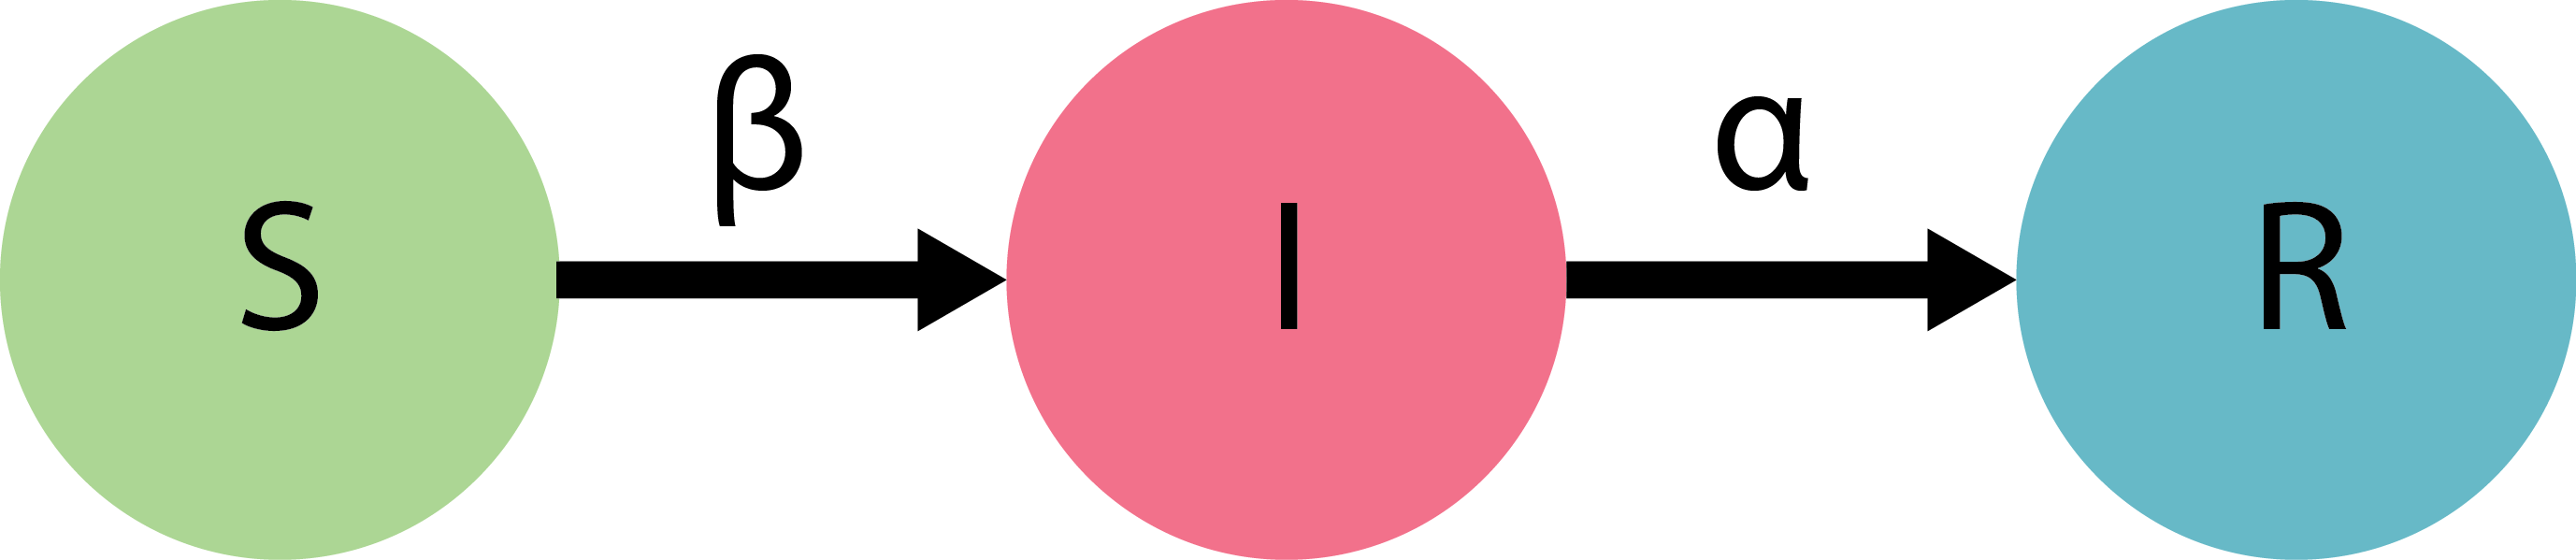
\includegraphics[width=\linewidth]{compartmental-models/SIR-compartments.png}
	\caption{Flowchart of the Kermack–McKendrick SIR epidemic model. The circles represent the compartments and the arrows show allowed transfers between them with the associated parameters of transfer rates above.}
\end{figure}
\\
Eq. (\ref{SIR1}) is justified by noting that the infection rate is positively correlated to the number of contacts between $S$ and $I$. We then use the law of mass action from assumption \ref{SIR-as-ma} to say that the number of contacts between infectives and susceptibles is proportional to the product of the size of the two interacting classes, $SI$. Introducing a proportionality constant $\beta>0$, we can say that $\beta SI$ individuals are infected per unit time. Here $\beta$ denotes the \textit{transmission rate}\footnote{Note there are different ways of defining $\beta$ that lead to a different dynamical system. The other popular way is to define $\beta$ in a way that leads to $\dot S=-\frac{\beta S I}{N}$. This has some potential benefits but it obscures the pedagogy.}. $\beta$ is a parameter that is the product of how often contacts between susceptible and infective individuals occur, $c$, and the probability that a contact leads to infection, $p$.\\
\\
Eq. (\ref{SIR3}) is found by assuming that the number of individuals getting better is proportional to the amount of individuals who are ill. We let $\alpha>0$ be the proportionality constant. This in effect assumes that the infective period has an exponential distribution\footnote{Let $u(s)=$ number of infective individuals at time $s$ after having been infective. Then $\dot u=-\alpha u\implies u(s)=u(0)e^{-\alpha s}$}.  This is the \textit{transition (or removal) rate}, the rate that infective individuals are removed by either recovery and immunisation or death. Equivalently, it  means that the time of infectivity is exponentially distributed with mean $1/\alpha$.\\
\\
Finally, assumption \ref{SIR-as-pop} tells us that Eq. (\ref{SIR2}) is determined by the other two equations. Also, if we included any removed individuals at the start of system, they would play no part in the dynamics. So without loss of generality, we can assume $R_0=0$ in the initial conditions.
\subsection{Analysing the model}
Whilst it is possible to derive exact analytical solutions to this system\cite{exact-SIR}, it is simpler and far more instructive to explore the qualitative behaviour and derive some important quantitative properties.\\
\\
Note that $R$ plays no role in the equations of $\dot S$ or $\dot I$. Therefore we can consider just these two coupled equations\cite{martcheva}. If we need $R$ we can easily get it back by using assumption \ref{SIR-as-pop} that $R=N-S-I$. Decoupling $R$ gives the 2-dimensional system:
\begin{eqnarray}
	\dot S=-\beta S I\label{red-SIR1}\\
	\dot I=\beta S I-\alpha I=(\beta S-\alpha)I\label{red-SIR2}
\end{eqnarray}
with initial conditions: $S(0)=S_0,I(0)=I_0, S_0+I_0=N$.
%\paragraph{Basic Dynamics}
\begin{figure}
	\centering
	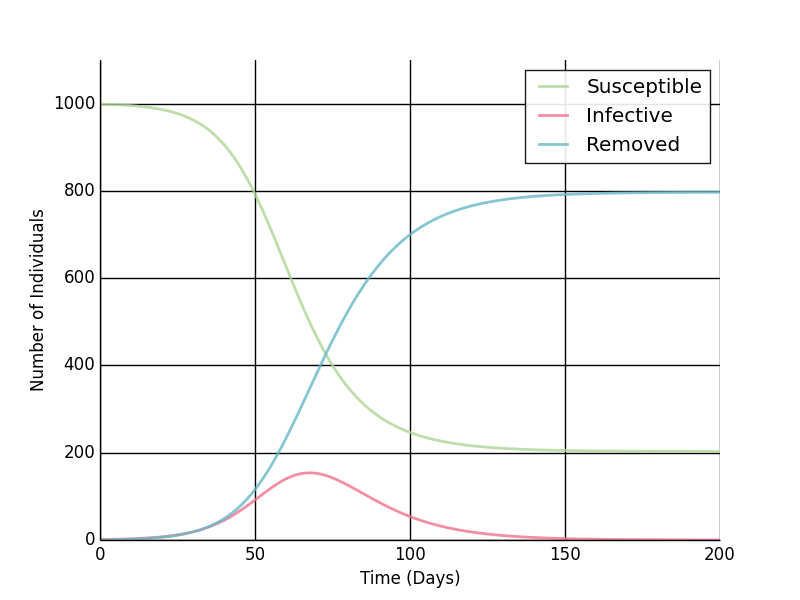
\includegraphics[width=1\linewidth]{compartmental-models/SIR-trajectory-fill.png}
	\caption{A typical SIR trajectory with $\beta=2\times10^{-3},\alpha=1/10, N=1000$}
\end{figure}
\subsubsection{Important quantities for epidemiologists}
Imagine you are the president of a country experiencing a significant epidemic. You have assembled a room full of leading epidemiologists to brief you. What do you ask them?
\subsubsection{Basic reproduction number, $R_0$}
Perhaps the first thing you will ask is: is the epidemic getting better or is it getting worse?\\
\\
As $\beta,S,I\geq 0$ it is immediate from Eq. (\ref{red-SIR1}) that $\dot S(t)=-\beta SI\leq 0$ for all $t$. That is the number of susceptibles is a decreasing function. Indeed if $S,I>0$ then it is strictly decreasing. So the number of susceptibles decreases until there are either no susceptibles or no infectives.\\
\\
Also, we have \[\dot I=(\beta S-\alpha)I>0\iff\beta S-\alpha>0\iff S>\alpha/\beta\] So $I$ increases only if $S>\alpha/\beta$. If $S_0<\alpha/\beta$, $I$ decreases for all $t$ and the infection dies without any increase in infection cases. Alternatively if $S_0<\alpha/\beta$, $I$ begins by increasing. But as established, $S$ is strictly decreasing for $I\neq0$ so $S$ decreases until eventually $S=\alpha/\beta$. At this point $I$ will reach a maximum. For all $t$ after this it will decrease to the limit $I=0$.\\
\\
From the arguments above $\beta S-\alpha$ plays a key role in the dynamics. We define the basic reproduction number $R_0=\beta S_0/\alpha$\cite{models-epidemiology-2}. Note that if $R_0>1$ the number of infective individuals will increase at time $t=0$. In this case we say that there is an epidemic. If $R_0\leq1$ the infection dies out without any increase in the number of infected individuals at any point.\\
\\
There is some disagreement among biologists and mathematicians over the exact definition and interpretation of $R_0$\cite{Heffernan281}. However, most models assume that $S_0\approx N$. This can be motivated by considering how an epidemic can begin. We can imagine a member getting infected through travel for example and returning to the population. Then $I_0=1$ and $S_0=N-1$. As we usually consider $N\gg1$ we have $S_0\approx N$. This assumptions allows us to consider $R_0$ as the number of infections passed on by a single infective individual during their infective period in a completely susceptible population.\label{mm}\\
\\
%Intuitively, $\beta S_0/\alpha$ is the number of infections passed on by a single infective individual during their infective period in the initial population.
%\textit{Mark's note- The population doesn’t need to be completely susceptible, does it? That would amount to defining $R_0$ as $R_0 = \beta N / \alpha$.}
%As models usually assume that $S_0\approx N$, it can also be considered as the number of infections passed on by a single infective individual during their infective period in a completely susceptible population\cite{models-epidemiology-2}.
This interpretation is easily understood. $\beta S$ is the rate of new infections caused by infections caused by a single infective individual. The mean length of an infective period is $1/\alpha$ by the assumption of exponentially distributed infections lengths. If an infected individual is, on average, not able to pass it on to at least one other person clearly the the infection will die out.
\subsubsection{Final size relation}
The next question you, as President, may ask is: how many people will the epidemic affect? This is given by the final size relation, an equation relating the number of affected individuals to $R_0$. Recalling that $\dot S\rightarrow0$ as $t\rightarrow0$, we can define $\lim_{t\rightarrow\infty}S(t)=S_\infty$. The number of individuals affected by the epidemic is the total number of individuals who have been infected at \textit{any} point. That is equal the size of the population minus the still susceptible population: $N-S_\infty$\label{mmd}. It can be shown that\cite{models-epidemiology} \[N-S_\infty=\frac{N}{R_0}\log(\frac{S_0}{S_\infty})\]
This is often written in the form \[\log(\frac{S_0}{S_\infty})=R_0(1-\frac{S_\infty}{N})\]\label{mmd} and called the \textit{final size relation}.
\subsubsection{Important quantities for revolutions}
The final size relation is an important quantity when studying infectious diseases because we care about the total number of affected individuals \textit{throughout} the diseases spread. However, in models of political revolutions it is of limited relevance. Instead we are interested in the amount of people active in sharing an idea at a single \textit{instant}. Instead of the epidemiological-minded \textit{final} size relation, we want a \textit{maximum} size relation. This would give a way of relating $R_0$ to the maximum size of the infective class $I_{\max}=\sup_{t\geq0}I(t)$.\\
\\
Firstly, let the infectious disease be the idea of a specific anti-regime group or movement. Let $S$ be the class of people who have not heard of this specific movement or have not been so far convinced by it. $I$ is the class of people who are convinced and actively sharing the ideas and taking part in revolutionary actions. Finally $R$ is the class of people who have been jailed, injured, fled the country or otherwise given up on actively supporting the cause.\\
%MM expand and slow down from here on out
\\
We assume that a revolution is successful if the proportion of active revolutionaries in a population is greater than some threshold value $r$ at some point. Formally, it is successful if there exists $t$ such that ${I(t)}/{N}\geq r$. This assumption of a threshold, whilst perhaps seeming oversimplistic, is backed by research\cite{logic-non-violence}. Further, this research suggests that the percentage of a population needed for a successful revolution is surprisingly small: just $3.5\%$\cite{logic-non-violence}. Some revolutions far surpass this number with an estimated $16\%$ of the Tunisian population actively participating in civil resistance in 2010\cite{arab-spring-percent}. While the analysis of this paper will not depend on the exact value of $r$, we will often use these two values $r=0.035$ and $r=0.16$ to get some values out of the derived equations.\\
\\
%MM expand a bit
As discussed, if $R_0\leq 1$ then no epidemic occurs and $I$ is decreasing for all $t$. In this case $I_{\max}=I_0$. So we assume $R_0>1$. Therefore we have $S_0>\alpha/\beta$. We define $t'>0$ to be the time such that $\dot S(t')=0$. Then $S(t')=\alpha/\beta$. From the previous arguments, $I(t)$ is increasing for $t$ when $0 \leq t<t'$ and decreasing for $t$ when $t'\leq t$. So $I$ reaches its maximum at $t'$. Formally, we have $I_{\max}=I(t')$.\\
\\
In mathematical epidemiology there is a classical equation to describe the maximum value of the infected class throughout the epidemic\cite{martcheva}:
\begin{equation}\label{eqn:imax}
	I_{\max}=S_0+I_0-\frac{\alpha}{\beta}+\frac{\alpha}{\beta}\ln\left(\frac{\alpha}{\beta}\right)-\frac{\alpha}{\beta}\ln(S_0)
\end{equation}\label{mmd}
This is very useful in modelling disease. If one can calculate $I_{\max}$ for a disease in its early stages, one is able to tell when the number of infections will decline\cite{martcheva}. However, we can adapt it to revolutions further.
\subsubsection{Maximum size relation}
Eq. (\ref{eqn:imax}) defines a subset of 4-dimensional space in $I_0\times S_0\times\alpha\times\beta$ with each point either leading to a revolution or not. This number of variables is acceptable if we know the specific parameters and are using it to calculate a value of $I_{\max}$. However, we can reduce it down further to 1-dimensional space in $R_0$ to obtain a more analytical insight.
\begin{align*}
I_{\max}&=S_0+I_0+\frac{\alpha}{\beta}\left(\ln\left(\frac{\alpha}{\beta}\right)-\ln(S_0)-1\right)\tab &\text{from \ref{eqn:imax}}\\
&=S_0+I_0+\frac{\alpha}{\beta}\left(\ln\left(\frac{\alpha}{\beta S_0}\right)-1\right)\tab &\text{by log rules}\\
&=S_0+I_0+\frac{\alpha}{\beta}\left(\ln\left(\frac{1}{R_0}\right)-1\right)\tab &\text{as } R_0=\frac{\beta S_0}{\alpha}\\
&=N+\frac{\alpha}{\beta}\left(\ln\left(\frac{1}{R_0}\right)-1\right)\tab &\text{as }S_0+I_0=N\\
&=N+\frac{\alpha}{\beta}(-\ln(R_0)-1)\tab &\text{by log rules}
\end{align*}
Recalling that a revolution happens if $I_{\max}/N\geq r$, we divide through by $N$:
\begin{align*}
\frac{I_{\max}}{N}&=\frac{N}{N}+\frac{\alpha}{\beta N}(-\ln(R_0)-1)\\
&=1+\frac{\alpha}{\beta N}(-\ln(R_0)-1).
\end{align*}
This is now in 3D space $\alpha\times\beta\times R_0(\alpha,\beta,S_0)$. To reduce it further we need to make an assumption. We assume that $I_0\ll S_0$ and thus that $S_0\approx N$. This can be motivated by supposing that, as we did for interpreting $R_0$, the revolutionary idea or movement comes from an individual or very small group or alternatively comes from outside the population of $N$ individuals. This allows us to write $\alpha/(\beta N)\approx \alpha/(\beta S_0)=1/R_0$. Then we can write \[\frac{I_{\max}}{N}=1+\frac{1}{R_0}(-\ln(R_0)-1)\]
Finally with a small rearrangement, we have what we can baptise \textit{the maximum size relation}:
\begin{equation}\label{eq:max-size}
	\frac{I_{\max}}{N}=\frac{R_0-1-\ln(R_0)}{R_0}:=m(R_0)
\end{equation}
valid for $R_0\geq1$.\\
\\
Bringing this together, we say a revolution occurs if and only if \[m(R_0)=\frac{R_0-1-\ln(R_0)}{R_0}\geq r \text{ for a given } r\]
\begin{figure}
	\centering
	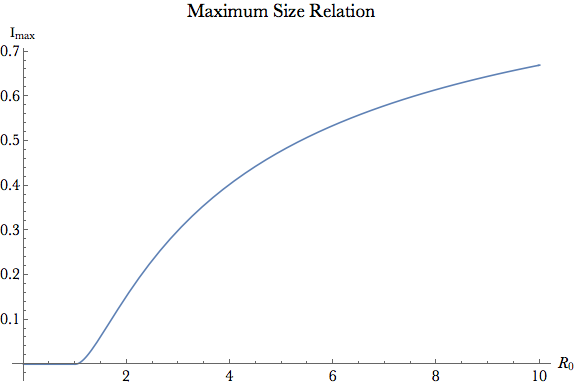
\includegraphics[width=0.95\linewidth, trim={0, 0 0 0.7cm}, clip]{/compartmental-models/maximum-size-relation.png}
	\caption{Graph showing how the maximum fraction of infectives in the population varies with the basic reproduction number $R_0$ in the SIR model. This is derived from the maximum size relation (Eq. (\ref{eq:max-size})). Note in particular how small values of $R_0$ can result in significant fractions of the population being active at the revolution's peak.}
\end{figure}
We can check that the proposed maximum size relation has desirable properties in relating $R_0$ to $I_{\max}/N$. The domain should be $R_0\geq 1$ as we excluded lower values in the derivation. Also as $I_{\max}/N$ is a proportion, we need to ensure that the codomain is restricted to $0\leq m(R_0) \leq 1$. We also presume that the higher $R_0$, the higher the value of $m(R_0)$. So to summarise this, we want an increasing function $m:[1,\infty]\rightarrow[0,1]$.\\
\\
It is increasing as \[\frac{d(I_{\max}/N)}{dR_0}=\frac{\ln R_0}{R_0^2}\geq0, \forall R_0\geq1\]
We also have $m(R_0=1)=0$. Further, as $R_0$ tends to infinity, $\lim_{R_0\rightarrow\infty}m(R_0)=1$\label{mmd}. As $m$ is an increasing function, these give the minimum and maximum respectively. So the proposed maximum size relation has all the desired properties.\\
\\
We can provide some intuition for the maximum size relation by interpreting the $\frac{R_0-1}{R_0}$ term as how much over the threshold of $1$ $R_0$ is. Clearly the larger it is, the higher we can expect $I_{\max}$ to be. However, this potentially unlimited growth is inhibited by the ${-\ln(R_0)}/{R_0}$ term, representing the depletion of the susceptible population and thus a reduction in transfer rate $\beta S I$.\\
\\
Note that this analysis holds for the SIR model in general and can be used to roughly predict the number of infective cases that will be occurring at an infection's peak severity. This is useful in telling when an epidemic will begin to decay away. However if a researcher was calculating $I_{\max}$ from the SIR model, they would find estimate values of $\alpha,\beta,S_0,I_0$ and calculate $I_{\max}$ from Eq. (\eqref{eqn:imax}). In practice they would not use the SIR model but instead base these calculations on a more specialised model. However, for our analytical purposes it is very useful. We can interpret $R_0$ as the amount of people the average revolutionary would have to convince to be part of their movement if no one in the population had yet heard of the movement.\\
\\
If we desire a quick estimate of some values, we can naively apply the SIR model to the study of revolutions. As discussed earlier, research suggests that the threshold is given by $r=0.035$. Using the freshly created maximum size relation we see that to get to the critical value of an engaged populace needed for a revolution we need a basic reproduction number of $R_0=1.338$ . In other words, each revolutionary must be able to, if in a fully susceptible population, convince $1.338$ people to join the revolution before they are removed. For the Tunisian revolution in 2010 with $16\%$ of the population involved in the revolution\cite{arab-spring-percent}, solving Eq. (\ref{eq:max-size}) yields $R_0=2.04$.\label{mmd} This is a basic reproduction number comparable to that of the relatively uninfective Ebola\cite{b-r-n}.
\section{SEIR Model}
A simple and instructive modification we can make to the SIR model is to add a new class. Many infectious diseases have a period in which an individual can be \textit{infected} but not yet \textit{infective}. We call this state being \textit{exposed}. In our revolutionary interpretation, exposed individuals are those who have heard and are convinced by the revolutionary idea but are not yet presenting as active. We can represent this in a compartmental model by adding the exposed class $E$ to the SIR model, creating the SEIR model. 
\begin{figure}[h]
	\centering
	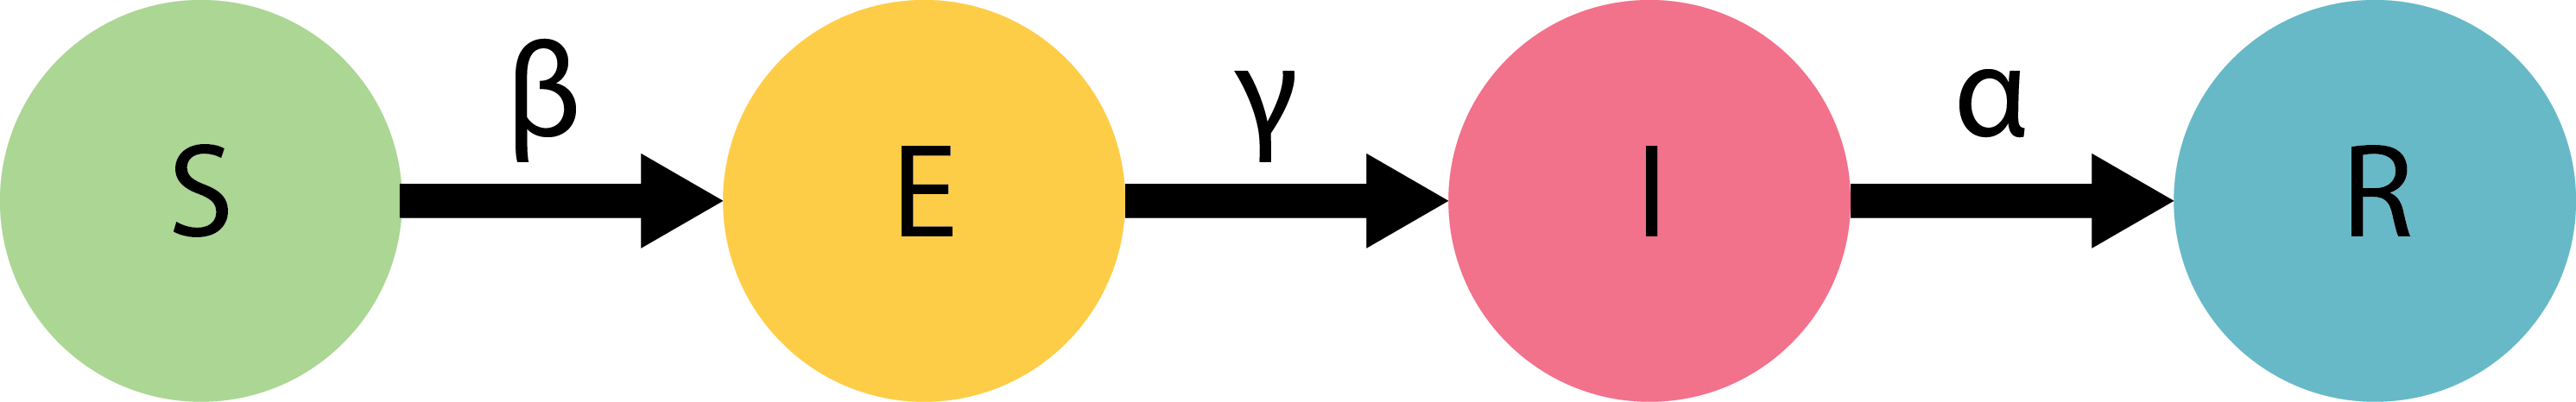
\includegraphics[width=\linewidth]{compartmental-models/SEIR-compartments.png}
	\caption{Flowchart of the SEIR epidemic model. Note that this is an extension of the SIR model that introduces an extra compartment $E$ and the transfer rate $\gamma$ between $E$ and $I$.}
\end{figure}

\subsection{Building the model}
We assume the exposed period is exponentially distributed with mean $1/\gamma$. Again this is equivalent to assuming that the rate of moving from $E$ to $I$ is proportional to the number of exposed individuals. This gives the dynamical system:\\
\begin{eqnarray}
\dot S=-\beta S I\\
\dot E=\beta S I-\gamma E\\
\dot I=\gamma E-\alpha I\\
\dot R=\alpha I
\end{eqnarray}
As before, we remove R to reduce the system by a dimension to give:\label{mmd}\\
\begin{eqnarray}
\dot S=-\beta S I\label{SEIR1}\\
\dot E=\beta S I-\gamma E\label{SEIR2}\\
\dot I=\gamma E-\alpha I\label{SEIR3}
\end{eqnarray}
\subsection{Analysing the model}
\begin{figure}
	\centering
	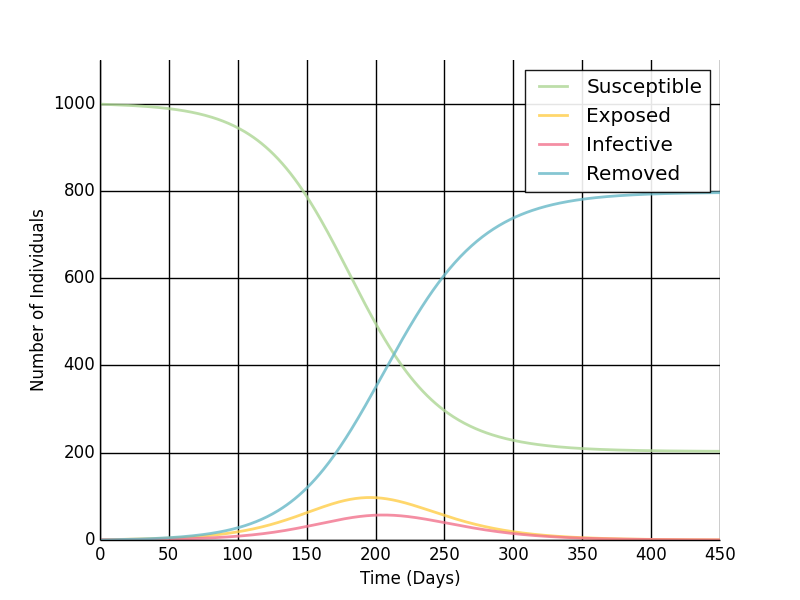
\includegraphics[width=\linewidth]{compartmental-models/SEIR-trajectory-fill.png}
	\caption{A typical SEIR trajectory with $\beta=3,\alpha=1/10,\gamma=1/300$}
\end{figure}
In the SIR model we could tell if an epidemic would occur simply by seeing if there was initial growth in the infective class. This worked because, if the infective class did not grow initially, it could not grow at any later time. However, the SEIR model is more complex and can have initial decline yet still see an epidemic. As we can no longer use our previous definition of an epidemic occurring we are motivated to develop a new, more general one.\\
\\
%Instead it is characterised by the equilibrium with all individuals of the population susceptible
One possibility is to consider the disease-free equilibrium (DFE). This is the equilibrium that occurs when the whole population is in the susceptible class. In the SEIR system (\ref{SEIR1}-\ref{SEIR3}) the DFE is given by $(S,E,I)=(N,0,0)$. It is easy to see that this is in fact an equilibrium in the SEIR system and gives $\dot S=\dot E=\dot I=0$. In fact in all reasonable deterministic epidemic models this is an equilibrium: if there is no-one with the infectious disease and no randomness in the model, there is no way for the disease to enter the population and so everyone will stay susceptible. So if no-one is infective with the disease no-one ever will be.\\
\\
We say that an epidemic occurs if a small divergence from the DFE results in the system moving away from the DFE. Otherwise if the system does not move further away from the DFE, we say no epidemic occurs. One way to motivate this is to consider what would happen if a small number of infectives were released into the population. If they are able to infect more people, an epidemic occurs and we move from the DFE. Otherwise, the number of infective individuals decreases until there are no more. Translating this into mathematics we say an epidemic occurs if the DFE is unstable and an epidemic does not occur if the DFE is asymptotically unstable \footnote{See Section \ref{dynamical-systems} for a primer on dynamical systems}\cite{models-epidemiology-2}.\label{aa}\\
\\
The stability of SEIR can be investigated by linearising about the DFE. To do this we calculate the Jacobian at the DFE, $\bf{x}^*=(N,0,0)$,\\
\[
\bf{J}_{(\bf{x}^*)}=
{\begin{bmatrix}
	{\partial \dot S \over \partial S} &
	{\partial \dot S \over \partial E} &
	{\partial \dot S \over \partial I} \cr 
	{\partial \dot E \over \partial S} & 
	{\partial \dot E \over \partial E} & 
	{\partial \dot E \over \partial I} \cr 
	{\partial \dot I \over \partial S} & 
	{\partial \dot I \over \partial E} & 
	{\partial \dot I \over \partial I}
\end{bmatrix}}
_{(\bf{x}^*)}
={\begin{bmatrix}
	{-\beta I} &
	{0} &
	{-\beta S} \cr 
	{-\beta I} & 
	{-\gamma} & 
	{\beta S} \cr 
	{0} & 
	{\gamma} & 
	{-\alpha}
	\end{bmatrix}}
_{(\bf{x}^*)}
={\begin{bmatrix}
	{0} &
	{0} &
	{-\beta N} \cr 
	{0} & 
	{-\gamma} & 
	{\beta N} \cr 
	{0} & 
	{\gamma} & 
	{-\alpha}
	\end{bmatrix}}
\]
\\
Then finding the eigenvalues we get the determinant and resulting characteristic equation
\[{\begin{vmatrix}
	{-\lambda} &
	{0} &
	{-\beta N} \cr 
	{0} & 
	{-\gamma-\lambda} & 
	{\beta N} \cr 
	{0} & 
	{\gamma} & 
	{-\alpha-\lambda}
	\end{vmatrix}}=-\lambda\big((-\gamma-\lambda)(-\alpha-\lambda)-\beta N\gamma \big)\]
So $\lambda=0$ is an eigenvalue. This corresponds to the line of equilibria in which $E=I=0$. This is the system in which every individual is either susceptible or removed.\label{mmd}\\
\\
The other eigenvalues are the eigenvalues of the matrix:
\[{\begin{vmatrix}
	{-\gamma} & 
	{\beta N} \cr 
	{\gamma} & 
	{-\alpha}
	\end{vmatrix}}\]
These have negative real part if and only if the determinant of the matrix is positive\cite{models-epidemiology-2}. The determinant $\gamma(\alpha-\beta N)$ is positive if and only if $R_0<1$. Note that the trace of the matrix is negative and so the negative eigenvalues correspond to the stability of the equilibrium and the failure of an epidemic to develop\cite{models-epidemiology-2}. Hence again, the stability of the equilibrium in the SEIR model again depends on if $R_0$ is greater or less than $1$.

%This has determinant $\gamma(\alpha-\beta N)$. As $\gamma>0$, the determinant is positive if and only if $\alpha-\beta N$ is positive which is equivalent to $R_0<1$. An equilibrium point is unstable if there exists an eigenvalue with positive real part. We also know that a matrix's eigenvalues have negative real part if and only if the determinant is positive. And so if $R_0<1$, the DFE is stable. Otherwise it is unstable. \label{aa}
%\textit{Mark's note: Your claim about the value of the determinant and the signs of the real parts of the eigenvalues is too strong and actually false for matrices of odd dimension. The simplest way to fix this is to say something like:
%“The eigenvalues of a two-by-two matrix may have negative real part only if the determinant is positive”.}
\label{mmd}
\section{Model of revolution}\label{sec:rev-compartment}
%We can adapt the SEIR model to make an explicit compartmental model of revolution. A natural question is to consider if the basic flow should be the same. \label{mmd}
\subsection{Building the model}
% need a bit introducing E and also the analogy explicitly.
% also should I change the names of the compartments? Or does that make it more complicated?
The intrinsic difference between the spread of an infection and the spread of an idea is an individual's agency. With a general idea, this agency is not particularly important and can be bundled up with the transmission rate $\beta$. This parameter $\beta$ tells us about the average individuals likelihood of spreading an idea. However, with a revolutionary idea this agency is intrinsic. Most people who hold a revolutionary idea do not only consider the idea and see if they want to share it. They will also check the surrounding environment to see if others are sharing the idea, what the danger to them is and what the likelihood of a successful revolution is. To account for this we need an activation rate that is a function of the population demographic.\\
\\
Specifically, exposed individuals who are thinking about becoming active revolutionaries will look at what percentage of the population are already active revolutionaries. This is given by $I/N$. Fellow exposed individuals are invisible as they are not making any actions that display their support for a revolution. So we want the activation rate to be a function solely of $I/N$. So far, we do not know the nature of this function. For now we denote it $g(x):[0,1]\rightarrow\mathbb{R}$.\\
\\
Given the context it is natural to wonder if our model should allow transfers from $E\rightarrow R$. This corresponds to people who became convinced that the revolution is desirable but have since gone off the idea without ever having become revolutionaries. Whilst this is certainly possible it turns out that this is neither conceptually nor mathematically necessary. Conceptually, an exposed individual, while exposed has no effect on the wider population, much like a removed individual. In particular, they do not contribute to the size of the infective class which is the value we care most about. As the outwards effect on the dynamics between exposed and removed is negligible, an exposed individuals change to removed has no outward effect on the dynamics. Mathematically, we can account for this by making the value we give for $N$ smaller by a fraction corresponding to the fraction of people we expect to move directly from exposed to removed.\label{mmd}
\begin{figure}[h]
	\centering
	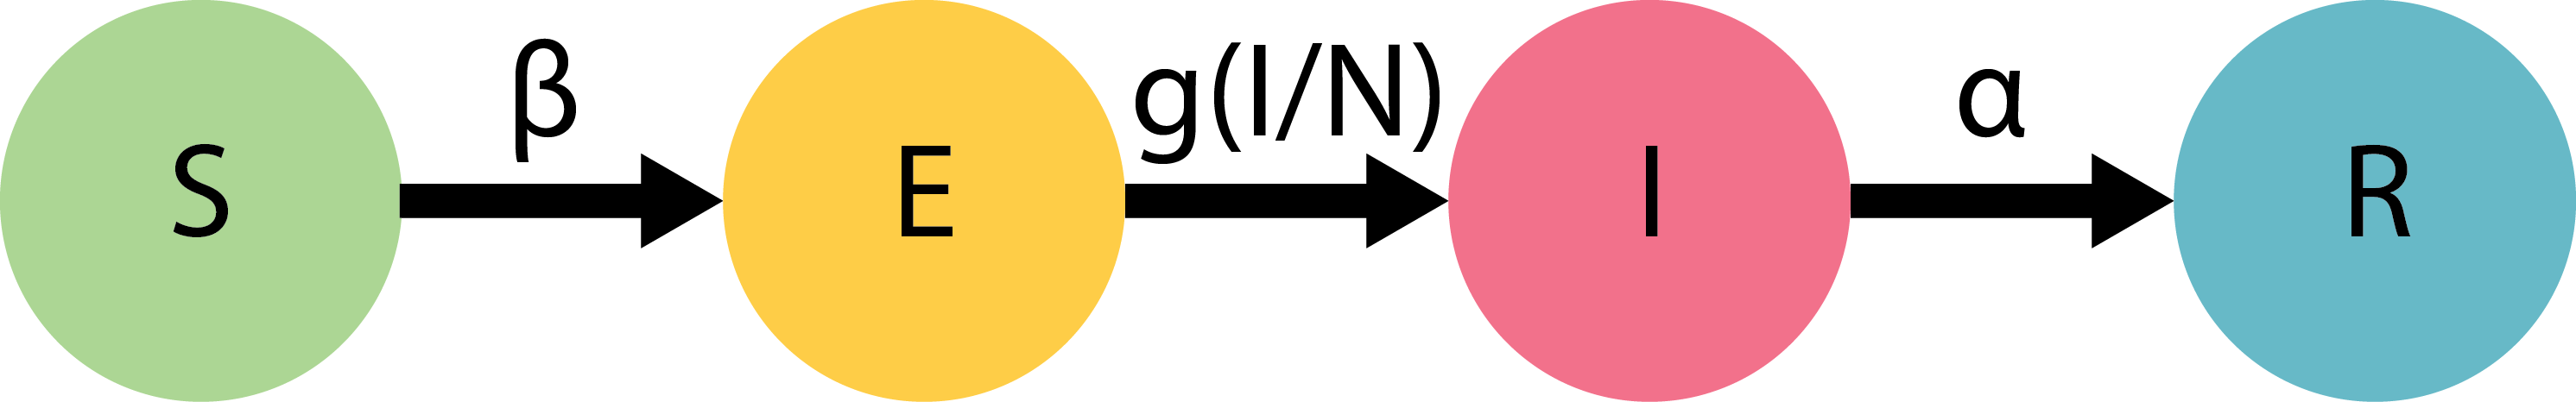
\includegraphics[width=\linewidth]{compartmental-models/rev-compartments.png}
	\caption{Flowchart of the compartmental model of revolution}
\end{figure}\\
\\
Adapting the SEIR model but allowing potential non-linear movement between the exposed and infective compartments, we get a dynamical system:
\begin{eqnarray}
\dot S=-\beta S I\\
\dot E=\beta S I- \gamma E g(I/N)\\
\dot I= \gamma E g(I/N)-\alpha I\\
\dot R=\alpha I
\end{eqnarray}
where $g(x)$ is the as yet unknown function.
\subsubsection{In search of $g(x)$: a naive approach}
The dynamics of collective behaviour are complex but there are some findings that are well-supported. People's proclivity towards behaving in a certain way often depends on how many people are already behaving that way. One of the dominant models of this in social psychology has been the threshold model. This holds that we tend to act in a certain way only if a certain number of other individuals are acting in that way\cite{threshold-models-social-influence}.\\
\\
Let $k$ be some threshold value with $0\leq k\leq1$. Then one option is to adapt the function from Granovetter's original paper on threshold models from absolute numbers of people to proportions of people. This would mean we have a discontinuous step function:\\
	\[
g_1(x) = \left\{\begin{array}{lr}
1, & \text{if } x\geq k\\
0, & \text{if } x< k
\end{array}\right\}
\]
where $k$ represents the threshold.\\
\\
A continuous alternative is given by:
\[g_2(x)=\frac{x^n}{k^n + x^n}\]
\begin{figure}
	\centering
	\begin{subfigure}{.46\textwidth}
		\centering
		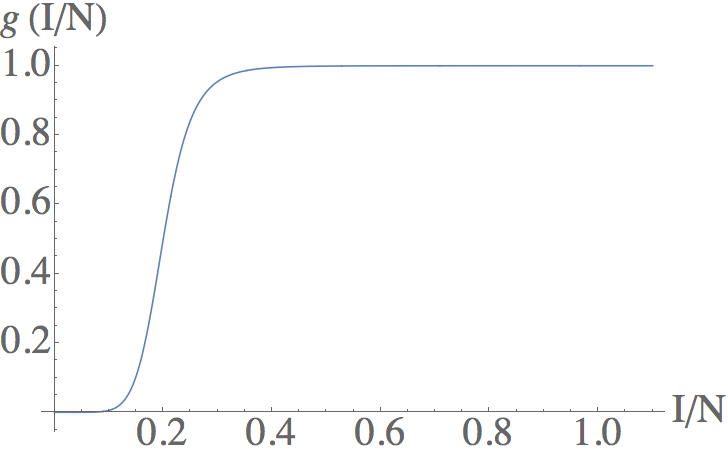
\includegraphics[width=\linewidth]{compartmental-models/rev-transfer-rate1.png}
		\caption{$n=2$}
	\end{subfigure}%
	\begin{subfigure}{.46\textwidth}
		\centering
		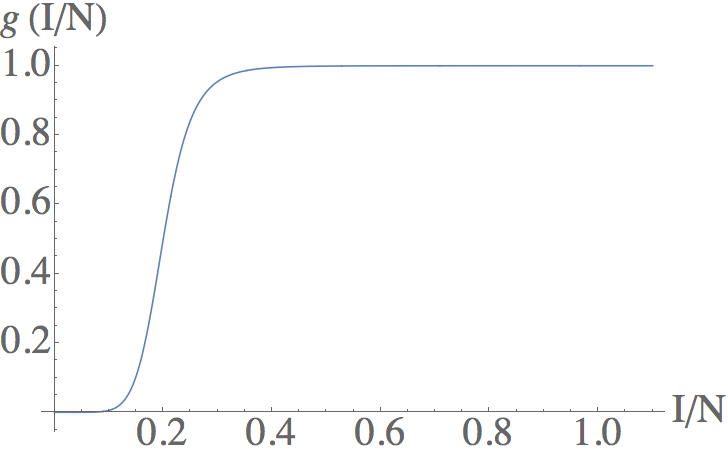
\includegraphics[width=\linewidth]{compartmental-models/rev-transfer-rate2.png}
		\caption{$n=7.5$}
	\end{subfigure}
	\begin{subfigure}{.46\textwidth}
		\centering
		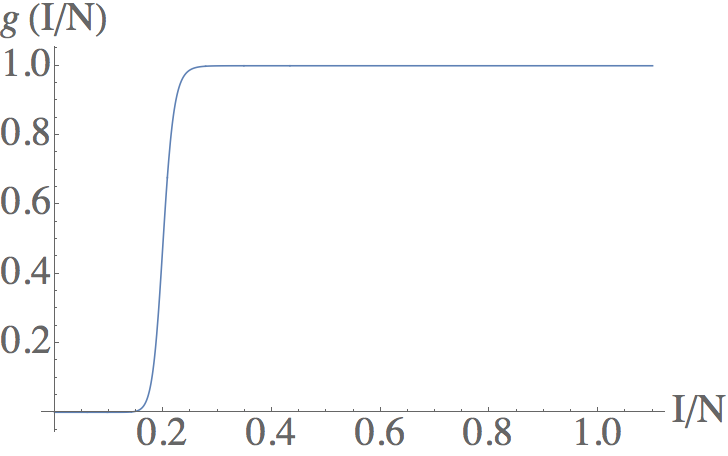
\includegraphics[width=\linewidth]{compartmental-models/rev-transfer-rate3.png}
		\caption{$n=20$}
	\end{subfigure}
	\caption{The effect of different values of $n$ on the transfer rate $g_2(x)$ with $k=0.2$.}
	\label{fig:transfer-rate-n}
\end{figure}
Here $k$ controls the threshold value with $g_2(x)={1\over2}$ at $x=k$. $n$ controls the severity of the threshold with a higher $n$ giving a steeper curve and a more sudden phase change. $g_2$ is preferable to $g_1$ both practically and theoretically. Practically, the continuity allows us to analyse the function at all points of the domain using standard calculus. Theoretically, it better represents the non-uniformity of a population's attitude to risk and the fuzzy boundary around giving an \textit{exact} threshold for active participation.\\
\\
We allow the possibility of scaling by a factor $\gamma$. Then $\gamma g(I/N)$ is the probability that an exposed individual will become active in one unit time. So if $I/N\approx1$, the probability of an exposed individual becoming active per unit time is roughly $\gamma$. This gives the number of individuals leaving $E$ per unit time as $\gamma Eg_2(I/N)$. So we have the dynamical system:
\begin{eqnarray}
\dot S=-\beta S I\\
\dot E=\beta S I- \gamma E \frac{(I/N)^n}{k^n + (I/N)^n}\\
\dot I= \gamma E \frac{(I/N)^n}{k^n + (I/N)^n}-\alpha I\\
\dot R=\alpha I\label{rev1eq4}
\end{eqnarray}
\subsubsection{Finding suitable parameters}
There are now 6 parameters in our model. We justify the default values used in Table \ref{tab:parameters1}. Unless otherwise stated, all simulations and graphs will use the values of the parameters as given in this table. For the initial conditions we start with a single revolutionary giving $I_0=1$ and $S_0=N-1$.
\begin{table}
	\captionof{table}{Default Parameter Values} \label{tab:parameters1} 
	\centering
	\begin{tabular}{| l | l | p{7.5cm} |}
		\hline
		Parameter (units) & Chosen Value & Justification \\ \hline
		N (people) & 2 million & $1/5$ of the population of Tunisia in 2010 (10.6 million). This is an estimate of how many people were potentially open to protesting (based on political orientation, age, medical history etc.).\\ \hline
		$\alpha$ (1/days) & 1/300 & Noting the exponential distribution inferred by Eq. (\ref{rev1eq4}), this assumes that a protester is removed through some means, on average, after 300 days of protesting. \\ \hline
%		$\beta$ (1/days$\cdot$people) & $2.04\cdot \alpha/N$ & Using $\alpha,N$ and the value of $R_0=2.04$ we calculated for the Tunisian revolution using the maximum size relation we get $\beta\approx\alpha R_0/N$. \\ \hline
		$\beta$ (1/days$\cdot$people) & $40\cdot \alpha/N$ & We assume that a revolutionary could expose around $50$ people to the idea in a completely susceptible population. Using the basic reproduction number we have $\beta\approx\alpha R_0/N$. \\ \hline
		$\gamma$ (1/days) & 1/5 & If conditions are right, it takes $5$ days on average for someone to move from exposed to active. \\ \hline
		$n$ (dimensionless) & 3 & This corresponds to a slightly steep curve of $g(x)$. \\ \hline
		$k$ (dimensionless) & 3/50 & The Asch conformity experiments found that an individual is highly influenced by 3 people to act in a way so as to conform with them\cite{asch-conformity}. However, increases to four and beyond have little effect. We assume each person is influenced by around $50$ people. \\ \hline
		$\delta$ (days) & $\gamma/200=1/1000$ & 
		We guess that around one in every 200 people is a potential `zealot'. If conditions are right, there are $1/\gamma$ people converting to active each unit time because of observing the population. There are 1/200 of the population converting who would have converted regardless of the political situation. \\ \hline
	\end{tabular}
\label{tab:parameters-compartments-1}
\end{table}

\subsubsection{Results and failure of the naive approach}
To keep things clean, we write \[\theta(I)=\frac{\partial g_2(I/N)}{\partial I}=\frac{k^n n (I/N)^n}{I(k^n+(I/N)^n)^2}\]
Decoupling $R$ as before, the Jacobian at the DFE
\[
\bf{J}_{(\bf{x}^*)}
={\begin{bmatrix}
	{-\beta I} &
	{0} &
	{-\beta S} \cr 
	{-\beta I} & 
	{-\gamma g_2(I/N)} & 
	{\beta S-\gamma E\theta(I)} \cr 
	{0} & 
	{\theta g_2(I/N)} & 
	{\gamma E \theta(I)-\alpha}
	\end{bmatrix}}
_{(\bf{x}^*)}
={\begin{bmatrix}
	{0} &
	{0} &
	{-\beta N} \cr 
	{0} & 
	{0} & 
	{\beta N} \cr 
	{0} & 
	{0} & 
	{-\alpha}
	\end{bmatrix}}
\] 
The resulting zero eigenvalues mean that we cannot ascertain whether it is a stable equilibrium. So we have to get creative. We could look at the Hessian, the square matrix of second order partial derivatives. However, this is a $9\times9$ matrix and we now have 6 parameters so this is neither fun nor informative. Instead we go exploring.\\
\\
The fact that there are zero eigenvalues suggests that the DFE is in fact part of an infinite number of equilibrium points. From observation, we can see that $(S^*,E^*,0)$ are all equilibrium points. These are the equilibriums in which there are varying degrees of revolutionary powder but no spark.\\
\\
To have an increase in the number of infectives we need the number of invididuals becoming infective to be greater than the number of those ceasing to be infective. Noting that $g_2(x)$ behaves like $n(\frac{x}{k})^n$ for small perturbations $x$ from $0$
\footnote{$g_2(x)$ has a Taylor expansion about $0$ of
\[g_2(x)=0+\frac{nk^nx^{n-1}}{(k^n+x^n)^2}\cdot x+...\approx \frac{nk^nx^{n}}{(k^n+x^n)^2}\] Noting that a small perturbation $x$ is much less than the threshold value $k$ we have $x\ll k$. Hence $k^n+x^n$ is dominated by the $k$ term. This gives the formula \[g_2(x)\approx\frac{nk^nx^n}{(k^n)^2}=\frac{nk^nx^{n}}{k^{2n}}=n\left(\frac{x}{k}\right)^n\]}. Therefore to have an increase in infectives we require that:
\begin{alignat}{2}
\gamma E n &\left( \frac{I/N}{k} \right)^n &&> \hspace{1.5em}\alpha I\label{eq:gamma-1}\\
&\hspace{1em}\gamma &&> \sqrt[n]{\frac{\alpha I}{E n}}k\frac{N}{I}\label{eq:gamma-2}
\end{alignat}
We know that $E<N$ and also that for $I$ to grow Eq. (\ref{eq:gamma-2}) must hold initially at $t=0$. So we can require $I=I_0=1$. Making these substitutions gives the requirement that
\begin{align*}
\gamma >& \sqrt[n]{\frac{\alpha}{N n}}k N
\end{align*}
If we use the default values to solve for $\gamma$, Eq. (\ref{eq:gamma-2}) gives a requirement that $\gamma>386$. This means that, on average, individuals become active less than $1/386$ of a day after having been exposed to the revolutionary idea. That is equal to four minutes which is barely enough to time to finish your cuppa.\\
\\
Therefore, we assume that with reasonable parameters the number of infectives is decreasing. So the only change can be that the active revolutionary dies and maybe some people become exposed to the idea. As we have $I_0=1$, the number of people who will be exposed is approximately equal to the number of people the active revolutionary can inform. That is exactly $R_0=\beta N/\alpha$.\\
\\
So we expect for any reasonable values, introducing a single revolutionary into the system will result in $I\rightarrow0$ as $t\rightarrow\infty$ while $E\rightarrow R_0$. This is in fact exactly what happens. With default parameters $R_0=2.04$ and so the revolutionary exposes two people to the idea before being snuffed out. Using a high value of $\beta$ as in Fig. \ref{fig:rev-naive-beta-high} we can visually see the system coming to its equilibrium point $(S^*,E^*,0)=(N-R_0,R_0,0)$.
\begin{figure}[!h]
	\centering
	\begin{subfigure}{0.8\textwidth}
	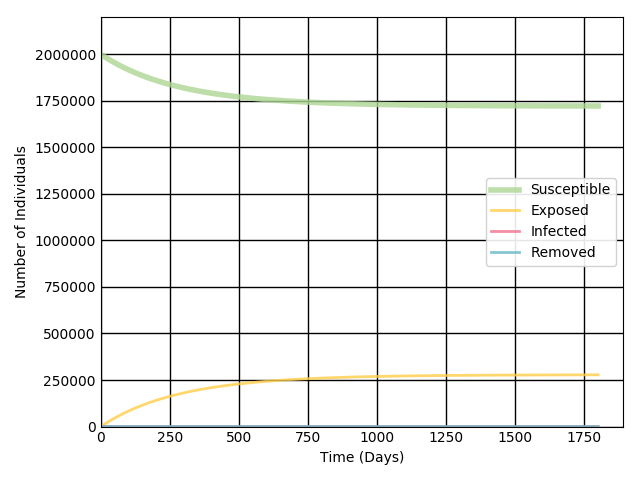
\includegraphics[width=\linewidth]{compartmental-models/failure-naive-approach3.png}
	\caption{A high, but still humanly possible, value of $\beta=1000/N$. This corresponds to each revolutionary exposing $1,000$ people a day to the revolutionary idea.}
	\label{fig:rev-naive-beta-high}
	\end{subfigure}
	\begin{subfigure}{0.8\textwidth}
		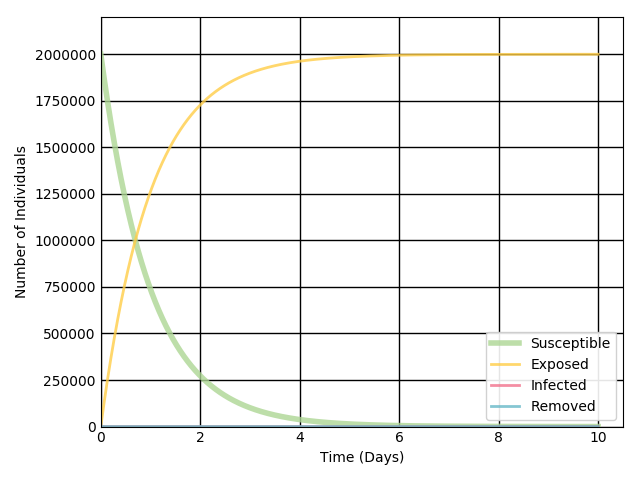
\includegraphics[width=\linewidth]{compartmental-models/failure-naive-approach2.png}
		\caption{A superhuman value of $\beta=1$. This corresponds to a revolutionary exposing roughly $1,000,000$ people to the revolutionary idea in a day.}
		\label{fig:rev-naive-beta-vhigh}
	\end{subfigure}
\caption{The compartmental revolution model with default parameters and high values of $\beta$. The resulting figures show the problems with the naive approach to the transfer rate $g(x)$.}
\end{figure}
\\
\\
Even if the active revolutionary is supernaturally effective, able to convince millions of people each day of the need for a revolution, he still suffers the same fate: dying whilst no other individual becomes active. This would involve having an unusually high transmission rate $\beta$. We set $\beta=1$, more than a million times the default parameter (Fig. \ref{fig:rev-naive-beta-vhigh}). Within two days we merely end up with the whole population convinced that they $\textit{should}$ do something. Meanwhile, the lonely active revolutionary becomes half a person, a third, reducing in size until he is infinitesimal. There is a powder keg of two million people but the only spark was left to die. Unfortunately, an idea without action remains just an idea.
%
\begin{tcolorbox}
	\paragraph{Lesson for revolutionaries:} An idea alone will never cause outward action. You must act in line with your beliefs to show others \textit{what} you believe. Otherwise everyone can believe in change yet do nothing about it.
\end{tcolorbox}
So in this model the most the revolutionary can hope for is to inform a lot of people that there \textit{should} be a revolution. Due to a limit on how quickly people move from being convinced of something to acting on it, there can never be an increase in the number of active revolutionaries.  This is a fatal problem for a model of revolution.\\
\\
Intuitively what has gone wrong is that when there is only one lone revolutionary, it's not particularly tempting to join them. The threshold model we have incorporated reflects the truth that most people do not want to be trend-starters. Most people, for better or worse, are sheep. However, fortunately change is possible. \textit{Most} people is not \textit{all} people.
\subsubsection{Improving $g(x)$: Thank God for the Zealots!}\label{sssec:zealots}
Some proportion of every society are zealots. They are the ones who are not afraid to stick their head above the pulpit. The fact that no one else is doing it does not faze them. In fact, they might actively enjoy it. These are the people who, upon hearing an idea they agree with, do not check to see if others hold and are expressing the idea. They simply express the idea. To get ourselves out of our rut, we assume that some proportion of the population are zealots.\\
\\
One option would be to introduce zealots as a category, with the majority of the population taking the traditional route route $S\rightarrow E\rightarrow I\rightarrow R$ and zealots perhaps moving directly $S\rightarrow I\rightarrow R$. However an alternative is to adopt this fraction of the population into the transfer rate $g$. This allows us to keep much of the analysis from the SEIR model.
%\textit{ Mark's note: This seems a good idea, but perhaps you should introduce zealots as a separate category of person who progress S -> I -> Rand then have the E -> I process depend on the sum of the population of ordinary Exposed people and the Infective Zealots.}
\label{mmd}
Then we choose instead \[g_3(x)=\delta+\gamma\frac{x^n}{k^n + x^n}\]
Note that this absorbs $\gamma$ into $g(x)$ so that it does not interfere with $\delta$. We can calculate a value of $\delta$ from imagining the transfer from $E$ to $I$ when the proportion of infectives $I/N$ is well past the threshold $k$. Then ${x^n}/({k^n + x^n})\approx1$ and the number of `ordinary' people per unit time who look at the population before deciding to be active is $\sim\gamma$. That is $\gamma$ people are converting for these reasons when the revolution is flowing per unit time. Similarly, $\delta$ people per unit time convert as `zealots' to the cause for reasons unrelated to the state of the revolution. Then we have have that the proportion of zealots in the initial population is given by $\delta/{(\delta+\gamma)}$\footnote{$\frac{\# \text{ zealots}}{\# \text{ individuals}}=\frac{\# \text{ zealots}}{\# \text{ zealots}+\# \text{ non-zealots}}=\frac{\delta}{\delta+\gamma}
%	=\frac{\gamma}{\delta+\gamma}$
$
}.
This gives us a way to find a meaningful value of $\delta$ (Table \ref{tab:parameters-compartments-1}).\\
\\
With this adoption the change in $E$ per unit time is given by:
\begin{equation*}\label{eq:g_3}
Eg_3(I/N)=E\cdot \big(\delta + \gamma\frac{(I/N)^n}{k^n + (I/N)^n}\big)
\end{equation*}
We can justify this term. The number of conversions to activity is proportional to the number of exposed individuals $E$. The first term in the brackets, $\delta$, represents those who, upon hearing an idea they agree with, become active regardless of the situation. The second term in the brackets $\gamma {(I/N)^n}/({k^n + (I/N)^n})$ represents the others who do a calculation by looking at what percentage of the population is active.\\
\\
It is worth noting that the value of $\delta$ is calculated using the fraction of zealots in the initial population. However this fraction changes as zealots are leaving the susceptible population at a different rate to the non-zealots in general this proportion will change during the revolution. This divergence is potentially a problem and difficult to justify analytically. However in practice, given the parameter values we use in the simulation, it has a negligible effect. Mathematically, the number of zealots who have become infective by time $t$ is $\int_0^t E\delta dt$. We will see in the model that in the early stages when zealots play the key role, $\int_0^t E\delta dt$ is very small compared to $N$ and so only a small amount of the total zealots have left the population.
%Similarly, the total number of individuals who have become infective is $\int_0^t Eg_3(I/N) dt$.
%Therefore, the fraction of the susceptible population that are zealots after time $t$ is at least as big as \[\frac{\delta}{\delta+\gamma}-\frac{\int_0^t E\delta dt}{N}\]
%in a population $\delta/{(\delta+\gamma)}$ should be altered by a factor that is at least close to $1$ as ${(N-\int_0^t E\delta dt)}/{N}$.
%So the effect of depleting zealots is only significant if $\int_0^t E\delta dt$ is comparable to $N$. We will return to see if this is the case in the simulations.
\label{mm}
\\
\\
Using $g_3$ results in the dynamical system:
\begin{eqnarray}
\dot S=-\beta S I\\
\dot E=\beta S I- E \left(\delta + \gamma\frac{(I/N)^n}{k^n + (I/N)^n}\right)\\
\dot I= E \left(\delta + \gamma\frac{(I/N)^n}{k^n + (I/N)^n}\right)-\alpha I\\
\dot R=\alpha I
\end{eqnarray}

\subsection{Analysing the model}
\subsubsection{Analytic results}
Reducing to three dimensions as before, the Jacobian at the DFE
$\bf{x}^*=(N,0,0)$ is\\
\[
\bf{J}_{(\bf{x}^*)}
={\begin{bmatrix}
	{-\beta I} &
	{0} &
	{-\beta S} \cr 
	{-\beta I} & 
	{-\delta-\gamma g_3(I/N)} & 
	{\beta S} \cr 
	{0} & 
	{\delta+\gamma g_3(I/N)} & 
	{-\alpha}
	\end{bmatrix}}
_{(\bf{x}^*)}
={\begin{bmatrix}
	{0} &
	{0} &
	{-\beta N} \cr 
	{0} & 
	{-\delta} & 
	{\beta N} \cr 
	{0} & 
	{\delta} & 
	{-\alpha}
	\end{bmatrix}}
\]
The addition of the `zealots' term makes the stability conditions of the revolution model reduce  to the conditions for the SEIR model. So by the arguments there, for a small disturbance from the DFE, there is no epidemic if $R_0<1$. However, from this we do not know how large the active population will grow. Further, it does not say anything about a large disturbance $I_0>0$ such that the non-zealot population becomes significant. To understand some of these details we need to create a simulation of the system.
\subsubsection{Simulation and qualitative results}
If we create a simulation of this system with the default values of the parameters we get something that looks a lot like how we may expect a revolution to occur (Fig. \ref{fig:rev-traj-default}). We can describe the course of the revolution in three distinct stages:
\begin{enumerate}
	\item\label{groundwork} \textit{The Groundwork}. Initially, the most notable increase is in the exposed population as the small infective population are able to make lots of contacts with the dominant susceptible population. However, there are not enough infectives to encourage others to become infective. Nevertheless, there is a small but reliable movement into the infective department through the existence of zealots. As this increases, the non-zealot term becomes non-negligible and the bolder non-zealots begin to crossover into the infective population. 
	\item\label{explosion} \textit{The Explosion}. Eventually the infective population becomes large enough to approach the threshold $k$ and suddenly the revolution sparks. The exposed population is quickly depleted, feeding quickly into the rapidly expanding infective population. The authorities are not quick enough to make a significant dint in the infective population so the removed population remains low. Within a short time, the susceptible population has been depleted and almost all of the population are active.
	\item\label{easy-pickings} \textit{Endgame} At this stage there are two possible outcomes.
	\begin{inparaenum}
		\item \textit{Change} If the infective class is large enough such that $I/N>k$ at some point, the revolution will have been successful. The dynamics go into another, far more difficult to model, phase of political movement: regime change.
		\item \textit{Easy Pickings} However, if the revolution is not able to pass the threshold, the regime stays in control. They are then free to pick at the revolutionaries who showed support for the revolution until they feel they have made a sufficient example of future would-be revolutionaries\footnote{Consider, for example, the 2016 Turkish coup d'\'etat attempt.}.
	\end{inparaenum}
\end{enumerate}
\begin{figure}[h!]
	\begin{subfigure}{\textwidth}
	\centering
	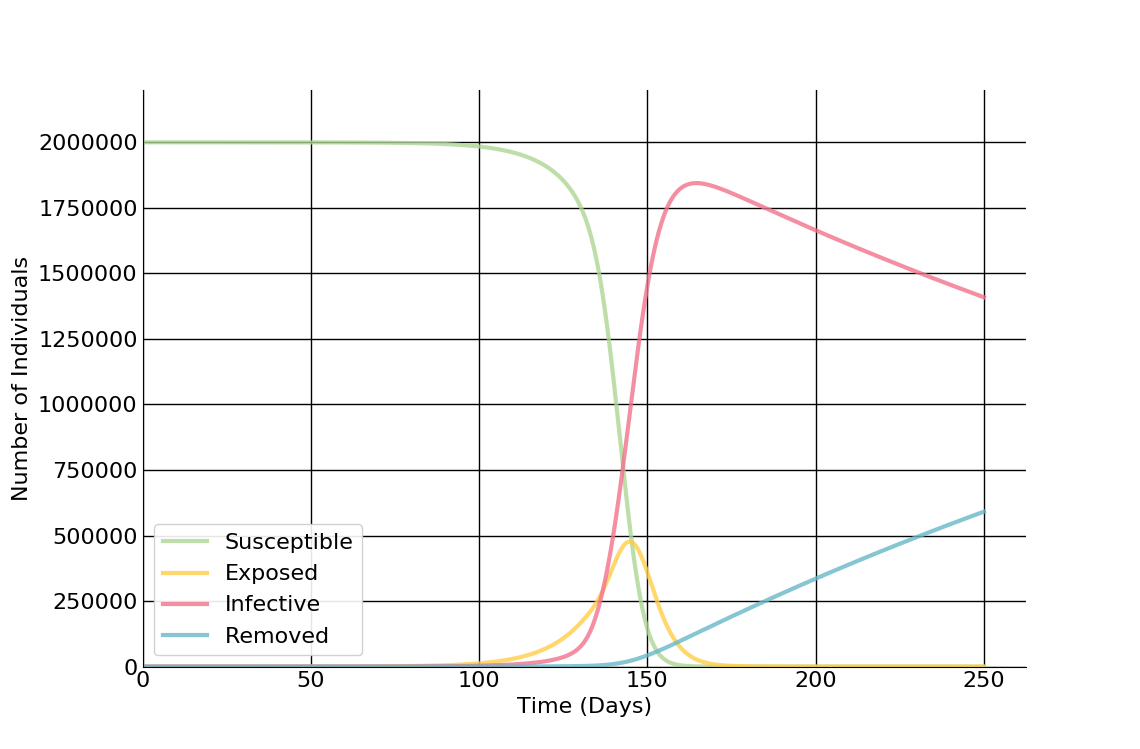
\includegraphics[width=\linewidth]{compartmental-models/rev-trajectory-fill1.png}
	\caption{With default parameters as given in table \ref{tab:parameters-compartments-1}.}
	\label{fig:rev-traj-default}
	\end{subfigure}
	\begin{subfigure}{\textwidth}
	\centering
	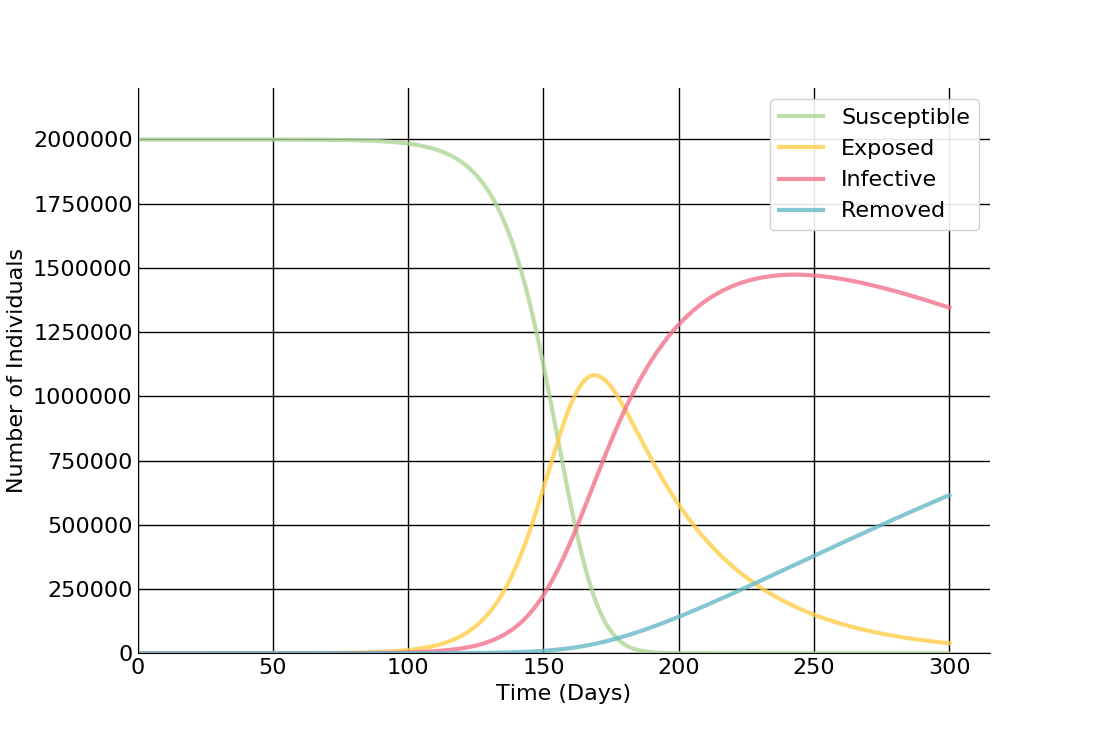
\includegraphics[width=\linewidth]{compartmental-models/rev-trajectory-fill2.png}
	\caption{With default parameters except $\gamma$ altered to $1/500$.
	}
	\label{fig:rev-traj-diff-gamma}
	\end{subfigure}
\caption{Trajectories of the compartmental revolution model.}
\end{figure}
\bigskip
Interestingly this story follows a similar narrative to George Lakey's strategy for nonviolent revolution in `A Manifesto for Nonviolent Revolution'\cite{lakey_1972}. In this he identifies five distinct stages for a successful revolution. The first two are cultural preparation or "conscientization" and building organizations. This educational phase roughly aligns with the `groundwork' stage we observe in our model. He sees confrontation and mass non-cooperation as the second two stages. This has a clear parallel with our 'explosion'. Finally the revolutionaries hope to enter the period `change' which Lakey identifies with the process of developing new institutions.\\
\\
%Returning to the discussion on the validity of our constant $\delta$ assumption we can see that in the early stages when it is mainly zealots converting, the total number of individuals who have been exposed by the time the zealots are the main contributors is very small. In later stages the effect of zealots is overran by the effect of zealots. So the assumption causes only a negligble change.\\
%\\
The simulation confirms the theoretical findings that $R_0$ plays a key role in the existence of an `epidemic'. That is, an increase in the number of active individuals. We can see that for $R_0<1$ no epidemic occurs whilst for values of $R_0$ even slightly above $R_0$ there is an increase in the infective population.
\subsubsection{The role of the contact rate $\beta$}
Further, the importance of $\beta$ is not surprising. A catchy idea catches on. It determines the size of the revolution and also how soon it happens. However, notice the danger of the \textit{good enough} idea as in Fig. \ref{fig:rev-R0-2}. This has $R_0>1$ but only just. As a result, the number of active revolutionaries sustains itself and can even have a small increase. However the amount leaving the cause or being picked off by the regime is almost equal to the amount joining at every point. This is a movement without momentum. It causes no major change but puts people at risk of the regime's wrath. In terms of wasted time and, depending on the nature of individual's removal, lives it is potentially worse than no agitation at all.
%\\
\begin{figure}[h!]
	\centering
	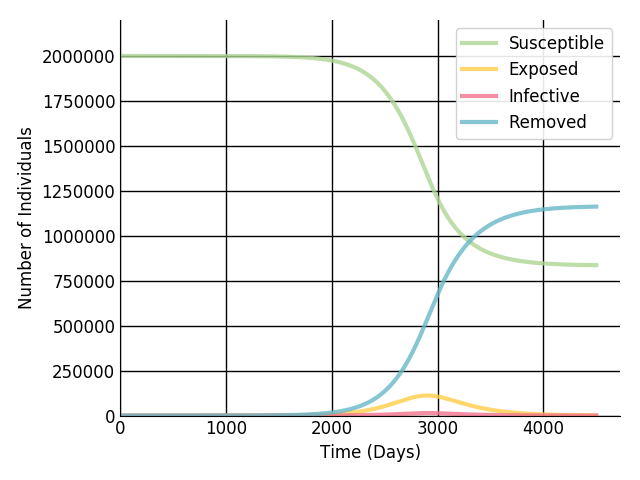
\includegraphics[width=1\linewidth]{compartmental-models/rev-R0-2.png}
	\caption{A graph showing the danger of the `good enough' idea on the revolution model. This has $R_0>1$ but only just.}
	\label{fig:rev-R0-2}
\end{figure}
	
\begin{tcolorbox}
	\paragraph{Lesson for revolutionaries:} Beware of the \textit{good enough} idea. It will not have the momentum needed to cause change. In the meantime it will put you in danger.
%	 If you're going to be active, make sure it's with a catchy idea. Otherwise you might die without seeing anything come of it.
\end{tcolorbox}
\subsubsection{The role of the removal rate $\alpha$}
There is an interesting link between $\alpha$ and $I_{\max}$, the key value we are interested in. Plotting $1/\alpha$ against $I_{\max}$ reveals that $1/\alpha$ has a non-linear effect on the maximum level of infection (Fig. \ref{fig:rev-alpha-not-log}). This suggests a logarithmic relationship. Indeed plotting this confirms this relationship for a large range of parameter values that includes our default value (Fig. \ref{fig:rev-alpha-log}).
\begin{figure}[h!]
	\begin{subfigure}{\textwidth}
		\centering
		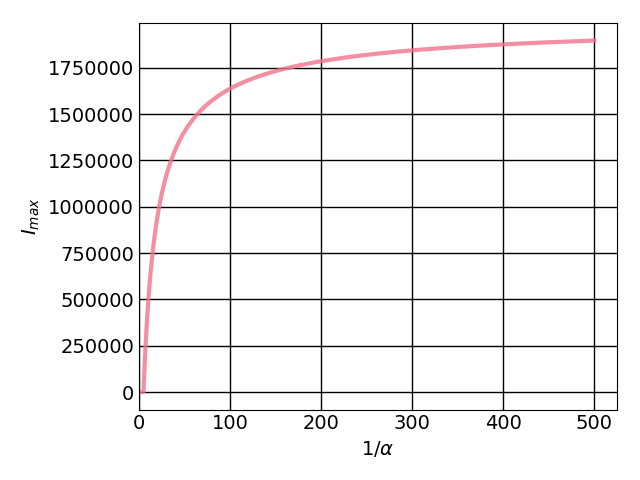
\includegraphics[width=0.8\linewidth]{compartmental-models/rev-alpha-not-log.png}
		\caption{There is a rapid increase in the value of $I_{\max}$ for small increases in $1/\alpha$ but this quickly settles.}
		\label{fig:rev-alpha-not-log}
	\end{subfigure}
	\begin{subfigure}{\textwidth}
		\centering
		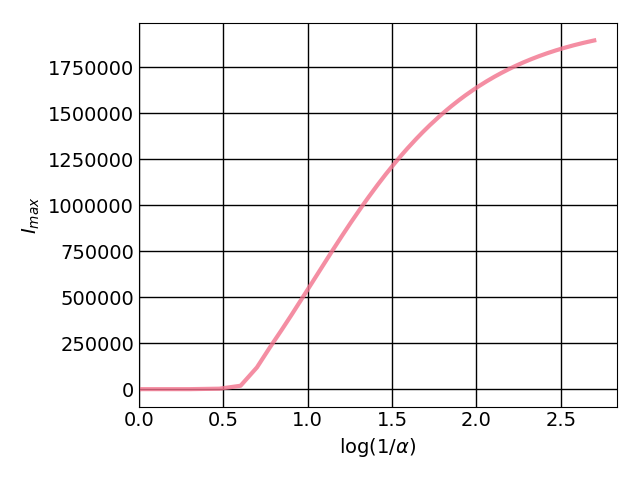
\includegraphics[width=0.8\linewidth]{compartmental-models/rev-alpha-log.png}
		\caption{There is an approximate log relationship between $1/\alpha$ and $I_{\max}$.}
		\label{fig:rev-alpha-log}
	\end{subfigure}
\caption{Graphs showing the effect the value of $1/\alpha$ has on the maximum infected class size. $1/\alpha$ represents the number of days on average it takes for a revolutionary to be removed.}
\end{figure}
%Investigate number of $I_0,E_0$ vs. $\alpha$ removal rate. Might be interesting to see relationship necessary to make something happen.\\
\\
\\
Perhaps even more interesting is the effect of $\alpha$ on the time of the peak of the revolution. Or better said, the lack of effect on it. It might be expected that if more people are leaving the revolution it will take longer to happen. However, this is not the case (Fig. \ref{fig:rev-alpha-time}). If the regime is picking people off any slower than a very fast rate, the peak of the revolution will tend to happen at a similar time. In our model this is around day $162$. In fact, even when $\alpha=0$, that is when no-one leaves the revolution, the peak of the revolution happens on day 162. So as $\alpha\rightarrow0$, the time of peak revolutionary activity $t$ tends to a limit and approaches it very quickly. Hence the time of revolution is not sensitive at all to our choice of $\alpha$.
\begin{figure}[h!]
	\centering
	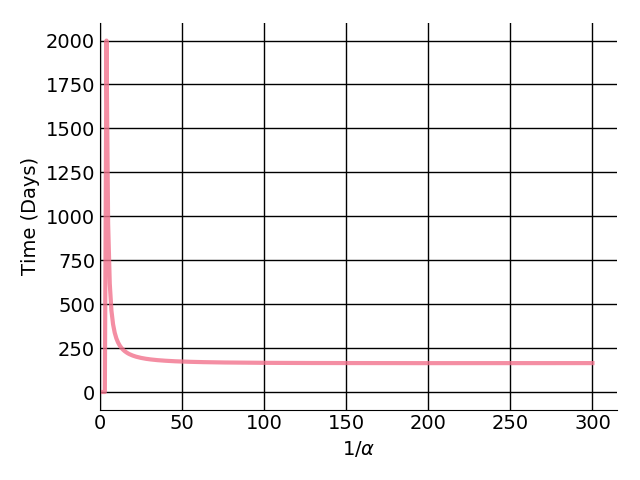
\includegraphics[width=1\linewidth]{compartmental-models/rev-alpha-time.png}
	\caption{A graph showing the lack of effect $\alpha$ has on the time at which the revolution peaks. That is the time $t$ at which $I(t)=I_{\max}$.}
	\label{fig:rev-alpha-time}
\end{figure}
\begin{tcolorbox}
	\paragraph{Lesson for revolutionaries:} The regime can't slow you down (unless they're really, really nasty). However, they will limit the size of the revolution.
\end{tcolorbox}
Note being nasty can be the same as increasing $\alpha$ but this might be intrinsic to the message of the revolutionaries. Therefore it might also involve increasing $\beta$. So tyrants play a tricky balancing act.
\begin{tcolorbox}[colback=removed-colour!30]
	\paragraph{Lesson for tyrants:} Being nasty (i.e. locking people up) will not move the revolution further away. Fortunately for you it will make the revolution smaller. However, it may also make it easier for revolutionaries to gather support against you. Maybe just be nice...?
\end{tcolorbox}
%\paragraph{$\gamma$ and $I_{\max}$}
\subsubsection{The role of the incubation rate $\gamma$}
$\gamma$, the parameter that controls the rate at which non-zealots convert to active revolutionaries, plays a key role in the time it takes for the revolution to happen and, for related reasons, the value of $I_{\max}$. $\gamma$ changes the relative heights of the peaks of $E,I$. If low ($\gamma\sim 1/500$), the growth of $E$ carries on for a long time and has time to grow very high (Fig. \ref{fig:rev-traj-diff-gamma}). Then $\sim1/\gamma$ days later we have the peak of the revolution where $I$ reaches $I_{\max}$. However, as $500$ days is a long time, the build-up to $I_{\max}$ takes a long time. As a result $I_{\max}$ is lower because people were picked off over a longer time. Compare this to Fig. \ref{fig:rev-traj-default}. Similarly, if $\gamma$ is even higher than default ($\gamma\sim1$), $I$ reaches the threshold quickly and then there is no time to remove people during the explosion period and so $I_{\max}\approx N$.
\begin{tcolorbox}
	\paragraph{Lesson for revolutionaries:} Pay attention to the political situation and other peoples' activity. Be ready to join quickly if the time is right.
\end{tcolorbox}
\subsubsection{Shortcomings of the model}
Exploring the simulation also shows the shortcomings of the model. With some parameter values we can witness values of $I<1$ that nevertheless result in an `epidemic'. In a discrete model, less than one revolutionary is no revolutionary. However, the continuity of the compartmental model can allow strange artefacts in which this fraction of a revolutionary manages to cause a revolution. We need something a bit more realistic.

\chapter{A stochastic agent-based network model}
\label{ch:abms}
\section{Agent-based models}
Agent-based modelling is a computational method that models interacting individuals in an environment using a `bottom-up' approach\cite{abm-gilbert}. The individuals are given preferences, actions available to them and ways to perceive not only themselves and their environment but also other agents. This method has proved useful in modelling a wide variety of complex systems in biology\cite{kroese-uppal}, social science\cite{epstein} and economics\cite{abm-economics}.\\
\\
Its utility derives from allowing researchers to solely define the characteristics of the individuals without saying anything explicit about the system they are trying to model. They then see what happens when those individuals are free to interact with each other and the environment in the ways defined. This lets researchers to model complex system-wide phenomena without making any system-wide assumptions.
\subsection{The components}
An agent-based model (ABM) has four essential elements: agents, the environment, the rules that define how the two of these work together and time.\\
\\
%agents
The agents can represent anything from an individual person to a company, from a bacteria to a country. Anything that has `agency' can be an agent in an ABM. That is, anything that has the ability to act. They are programmed to react to other agents, which may or may not be of the same type. So a person can interact with another person but could also interact with an agent that is a frog or a country.\\
\\
%Environment
The environment is a virtual world the agents both exist in and interact with\cite{abm-gilbert}. The environment may be abstract such as a network with the agents as nodes and an edge between two nodes signifying that those agents can interact with each other. However, it might also be very specific and concrete such as a geographically accurate rendering of a city.\\
\\
The rules bind these two elements. They define things like how many agents of each type there are in the environment, when agents can act and who with.\\
\\
%Time
For an ABM to be a useful model of a system by definition the agents need to act. For something to act, we need time to evolve. So time is an inherent part of ABMs. However, representing time in any computer program is a challenge. One can either approximate continuous time or be explicitly discrete. Due to the difficulties of approximating continuous time, most ABMs have time incrementing in discrete steps. We call the units of time \textit{ticks}.\\
\\
To make this a bit easy to grasp and see how it works in practice, we will look at one in-depth but simple example.

\subsection{Example: Boltzmann wealth model}\label{sec:boltzmann-wealth}
%\subsubsection{Introduction}
We will build a simple agent-based model to illustrate how they typically work. Taking a short break from the area of epidemiology and revolutions, we will try to model the unequal distribution of wealth in society. Econophysics is a trendy area of research, applying concepts from statistical mechanics to the study of economics\cite{econophysics2}. The model we will look at will be inspired by this area and, in particular, a model of Dr\u agulescu\cite{econophysics1} and Yakovenko\cite{boltzmann-tutorial}. The model is incredibly simple with only one type of agent, a minimal environment and just three rules. Despite its simplicity, this model can provide interesting and unexpected results.
\subsubsection{Setup}
%Agents, environment, time
In our model the agents are people. They have a non-negative integer amount of wealth $w\in\mathbb{N}^{\geq 0}$. They also have the ability to transfer money, if they have any, to other agents. The environment connects all agents to each other, allowing any agent to transfer money to any other. We will use discrete time in this model.\\
\\
%\paragraph{Rules}
The rules are simple:
\begin{enumerate}[
%	nosep,
%	label={Rule \arabic*}
	]
	\item\label{} There are $n$ agents.
	\item\label{} All agents start with $1$ unit of wealth.
	\item\label{} At each time-step, each agent that has at least one unit of wealth gives one unit to another agent, chosen randomly.
	\setcounter{rule}{\value{enumi}}
\end{enumerate}
\subsubsection{Implementation}
ABMs are essentially computer programs and so to implement the ideas above we need to write a program that will run in line with the set-up we have described.\\
\\
The implementation of an agent-based model typically has two main classes: the model and the agents. The model class defines the environment, the rules and controls time. It also holds the global variables such as the number of agents and is in charge of keeping track of all the agents. The agent class defines the interacting individuals. Typically this class will hold an agent's own properties and will define the functions that allow the agent to sense their environment and interact with other agents.\\
\\
%\paragraph{Implementing This}
The rules tell us what we need in the program.
\begin{enumerate}[
%	nosep,
%	label={From rule \arabic*}
	]
	\item\label{} We need the model class to hold an integer $n$, the number of agents in the model. We also need the model to have a way of creating agents.
	\item\label{} We need each agent class to hold the units of wealth that they have. We also need the model class to initialise each agent with $1$ unit of wealth.
	\item\label{} The agent class needs a function to distribute wealth. At each tick, if the agent has positive wealth, they decrease their wealth by 1 and increase the wealth of another agent by $1$.
\end{enumerate}
An example of a bare bones implementation of this is:
\lstinputlisting[language=python]{../Code/illustrative/boltzmann-wealth/bare-bones-1.py}
Note that we also assign each agent a `unique ID'. This is helpful for collecting data about the model, in particular for creating visual representations of the model or alternatively looking at typical behaviour of individual agents.
\subsubsection{Running the model}
We still need to add a few lines to make the code run and get a visual output. Letting it run for $100$ ticks with $100$ agents and plotting the results using
\lstinputlisting[language=python]{../Code/illustrative/boltzmann-wealth/bare-bones-2.py}
we get figure \ref{fig:single-init-1}.
\begin{figure}[h!]
	\centering
	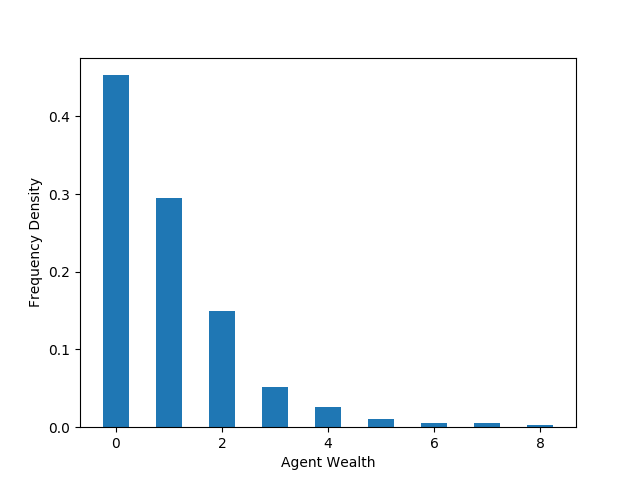
\includegraphics[width=.9\linewidth]{boltzmann-wealth/single-init-1.png}
	\caption{Graph of the density of agent's wealth after one $100$ step run of the Boltzmann wealth model with $100$ agents with initial wealth $1$}
	\label{fig:single-init-1}
\end{figure}
Though the program begins with the money equally spread throughout the population, it quickly becomes centred around a few very wealthy individuals. Around half of the population end up with nothing at all.\\
\\
%\paragraph{Batch Run}
The above graph was generated using just a single run of the program. One way we can get a clearer and firmer understanding of the system is to do `batch runs' where we run the simulation multiple times with the same parameters and compile all of the results. The following graph comes from running 100 of the simulations and creating a histogram of the wealth of the agents at the end.
\begin{figure}[!h]
	\centering
	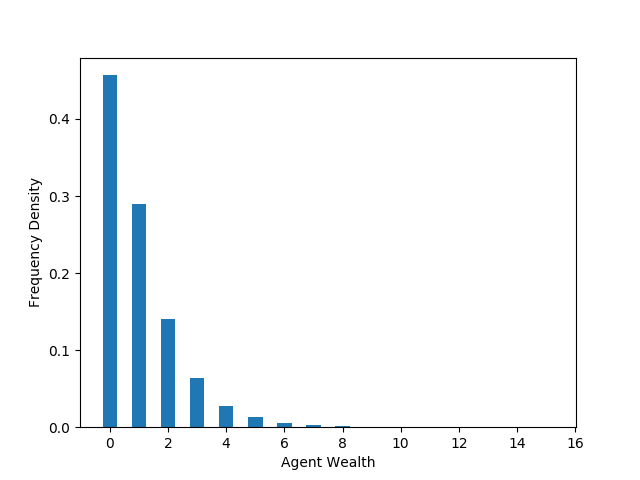
\includegraphics[width=.9\linewidth]{boltzmann-wealth/batch-init-1.png}
	\caption{Batch run of the Boltzmann Wealth model}
	\label{fig:batch-init-1}
\end{figure}
%would be cool to fit boltzmann curve to this
This shows the same disparity, perhaps even more starkly. Counter-intuitively, at least to me, despite having a constant process of redistributing wealth that seems to be in favour of the poor, we end up with a vastly unequal distribution. Almost half of all agents have 0 units of wealth while less than $10\%$ have $4$ or more. One agent in one of the runs ends with a wealth of $15$. Through a simple and easily comprehensible system we have found some intriguing results.\\
\\
One of the benefits of defining a social system as a program is that it makes it easy to run social experiments that would be difficult or unethical in real life. For example we can ask: what about if there is just more money around? Would that make the wealth distribution more equal? Exploring this is as easy as editing one initial value. If we start each individual with an initial wealth of $10$, though it takes longer to get there, we still end up with this inequality eventually. After 10000 ticks we end up with Figure \ref{fig:single-init-10}.
\begin{figure}[h!]
	\centering
	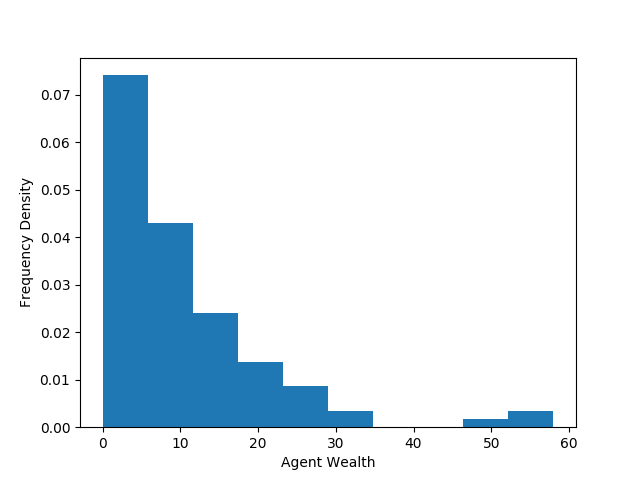
\includegraphics[width=.9\linewidth]{boltzmann-wealth/single-init-10.png}
	\caption{Histogram showing the result of increasing agent's initial wealth to $10$ on the Boltzmann wealth model.}
	\label{fig:single-init-10}
\end{figure}
So, in this system at least, economic inequality cannot be fixed by more money.\\
\\
We can then analyse this data as if it was field data. The fact that the distribution of wealth seems to move towards the same shape suggests some underlying equilibrium distribution. It turns out that the distribution of the wealth resulting from this model is actually a Boltzmann distribution\cite{dragulescu}. This is an exponential distribution typically linked to stochastic systems that try to reduce their energy potential.\\
\\
ABMs typically need some exterior reassurance that they are actually modelling the real world. Otherwise one can make many simplifications and assumptions and end up with a model that may or may not represent the system it is attempting to talk about. In this case one might consider real datasets of the income of a population. Indeed datasets show that income in the U.S.A. is distributed in a similar way to a Boltzmann distribution\cite{econophysics1}.\\
\\
If the data and model agree, researchers can use the model's results as evidence for bolder theses. In this case, researchers have argued that the Boltzmann distribution is in fact the \textit{expected} distribution of wealth in a capitalist society\cite{econophysics1}. The idea that this is a fundamental fact can be tested by seeing the result's robustness to different parameter values, rules and even different models. In this way, ABMs provide an interesting way to move back and forth between the world of theory and real world data.
\section{Social networks}
%\paragraph{Introduction}
In the Boltzmann wealth model the individuals exist in a very abstract space in which they interact with every other individual. In practice this is quite an unusual situation, as in general each person has some people they are more likely to interact with than others. People interact with the same people each day and have different relationships with others: friends, colleagues, stranger, daughter, spouse. This affects the interactions. This is also not unique to people. Companies, animals and countries have similar preferences and histories.\\
\\
We can consider each agent in a population as a node and we have an edge connecting two nodes if the two people have some form of social interaction such as friendship or acquaintance. This defines a social network\cite{networks}. An example of a social network is given by the author's Facebook friend network in Figure \ref{fig:facebook-network}.
\begin{figure}[h]
	\centering
	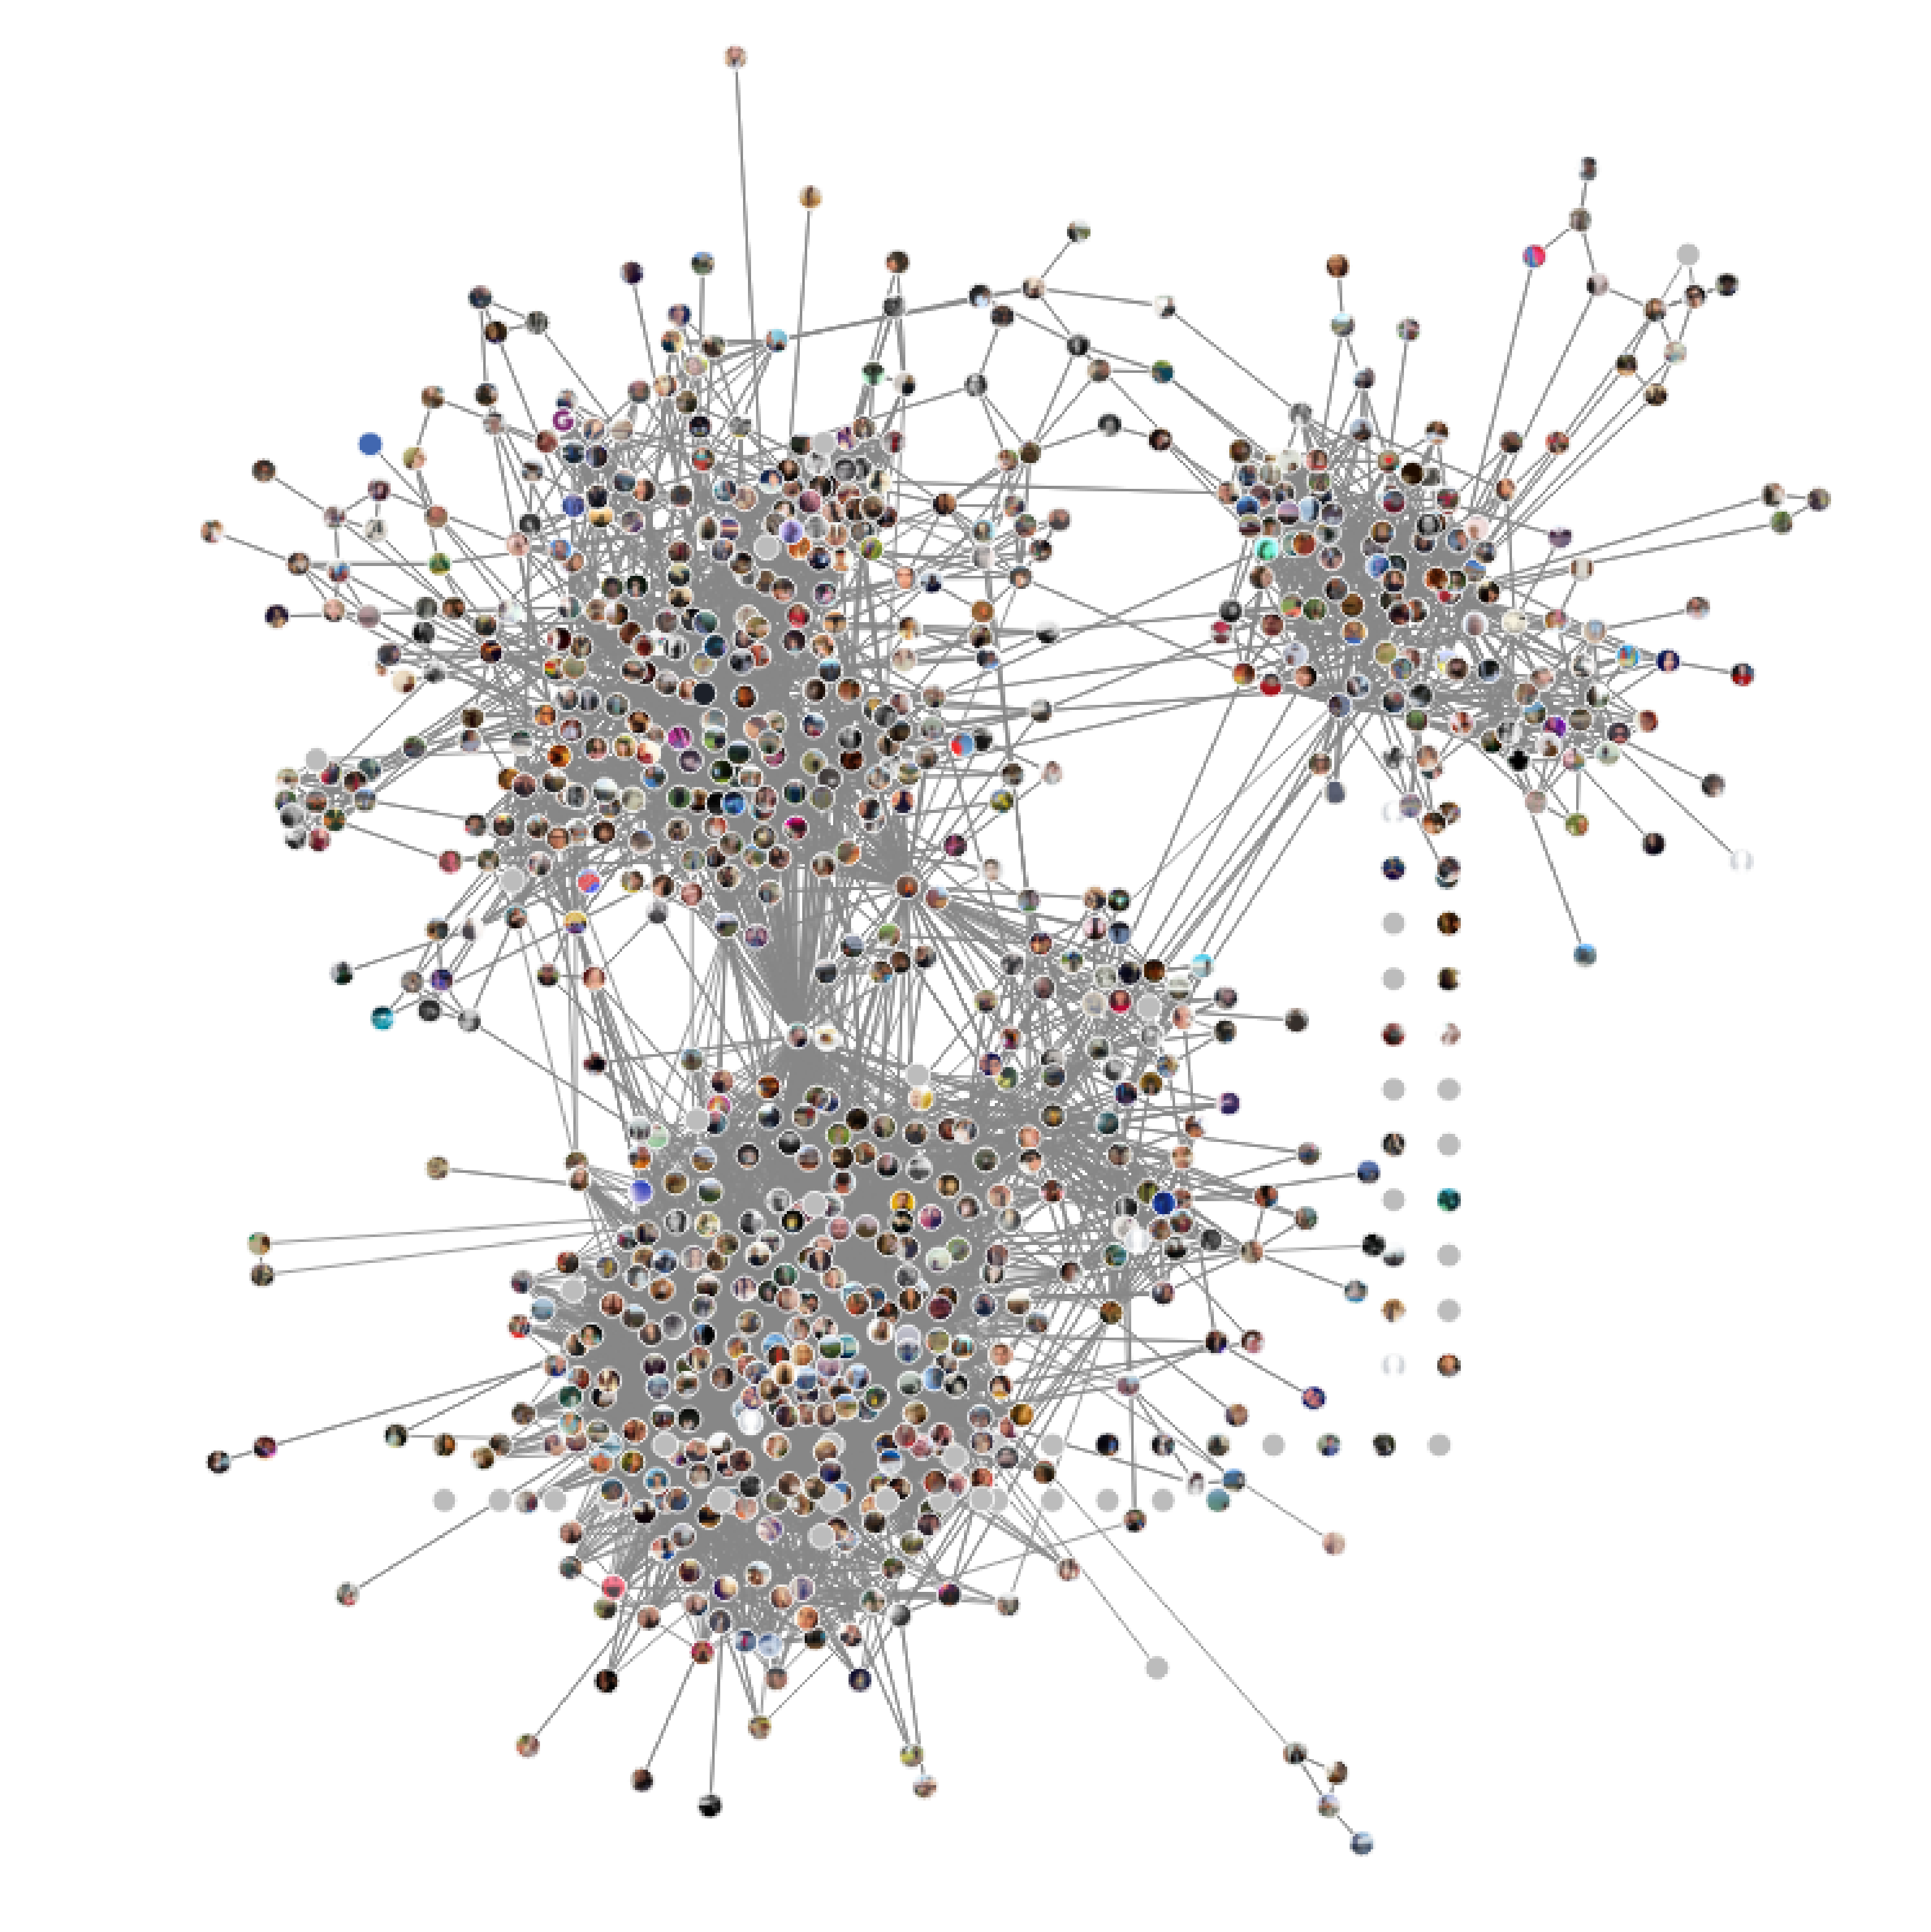
\includegraphics[width=.7\linewidth]{social-networks/joe-facebook-network-cropped}
	\caption{The author's Facebook friend network. Each node represents a Facebook friend and an edge between two nodes represents that those two people are friends on Facebook. Three main groups are revealed. The lower left contains people from Newcastle where I grew up. The top left are people from Manchester and university. The top right are people from Montreal where I studied for a year.}
	\label{fig:facebook-network}
\end{figure}\\
\\
For the success of an ABM that has a network structure underlying it, it is important to ensure that the network of the simulation accurately represents the features of a typical network. In particular for our case of modelling a revolution it is important to find a social network that accurately reflects the social graph of influence around transmitting political views and actions between citizens.\\
\\
There are two main ways we can find suitable networks to use in a model. Firstly, we can consider random graphs. These are a general species of graphs that are formed by a set of rules and reflect some aspect of real-life networks. The second option is to use datasets of real-life networks. Both have their merits and drawbacks.
\subsection{Random graphs}
%--Features of social networks: random, power-law tail, high clustering.--\\
A key feature of real-life networks is that they are irregular. They are much messier than well-ordered graphs such as complete graphs and lattices (see section \ref{sec:graph-theory}). To approximate this we need to look at graphs that can incorporate probability into some aspects of its structure. There are three main species of random graph we will look at: the Erd\H{o}s-R{\'e}nyi graph, scale-free graphs and small-world graphs.
%\\\\
%We also desire it to have a power-law tail and high clustering.
\subsubsection{Erd\H{o}s-R{\'e}nyi graph, $G(n,p)$}
The prototypical and perhaps simplest random graph is the Erd\H{o}s-R{\'e}nyi graph\footnote{Also known as the Poisson random graph, the Bernoulli random graph or simply the random graph.} $G(n,p)$. It is so prototypical it is often called \textit{the} random graph. It is defined in terms of two parameters: the number of nodes $n$ and the probability that there is an edge between any two nodes $p$. Figure \ref{fig:erdos-renyi-graphs} shows three graphs generated by this model.
\begin{figure}
	\centering
	\begin{subfigure}{.45\textwidth}
		\centering
		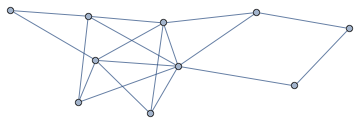
\includegraphics[width=1\linewidth]{erdos-renyi/G(10,0'5).png}
		\caption{$G(10,0.5)$}
		\label{fig:K5}
	\end{subfigure}
\begin{subfigure}{0.5\textwidth}
	\centering
	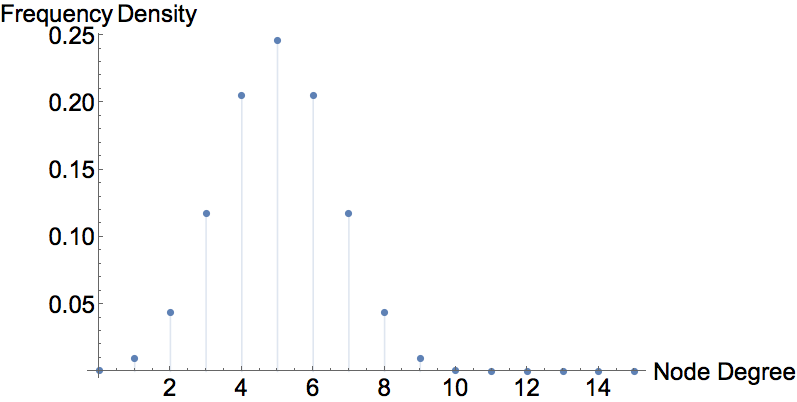
\includegraphics[width=1\linewidth]{erdos-renyi/e-r-prob-dist-1.png}
	\caption{$G(10,0.5)$}
	\label{fig:K5}
\end{subfigure}
	\begin{subfigure}{.45\textwidth}
		\centering
		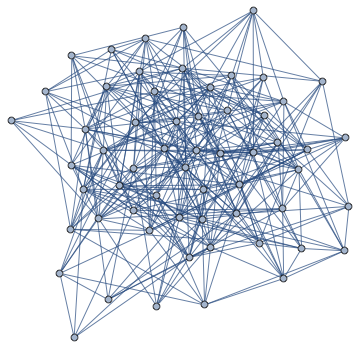
\includegraphics[width=1\linewidth]{erdos-renyi/G(59,0'2).png}
		\caption{$G(59,0.2)$}
		\label{fig:K16}
	\end{subfigure}
\begin{subfigure}{0.5\textwidth}
	\centering
	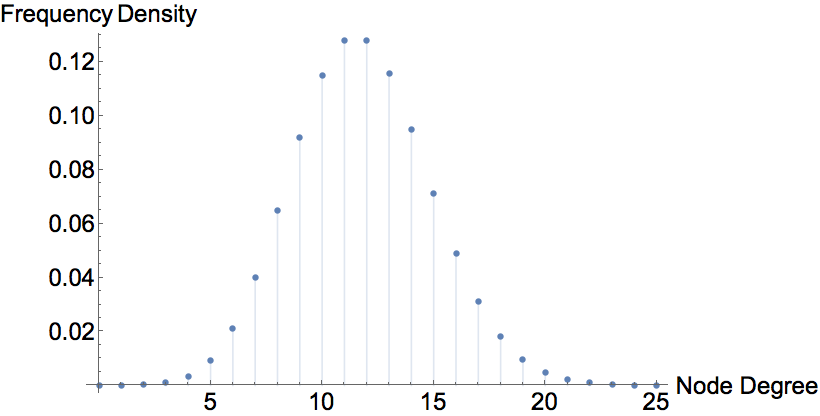
\includegraphics[width=1\linewidth]{erdos-renyi/e-r-prob-dist-2.png}
	\caption{$G(10,0.5)$}
	\label{fig:K5}
\end{subfigure}
	\begin{subfigure}{.45\textwidth}
		\centering
		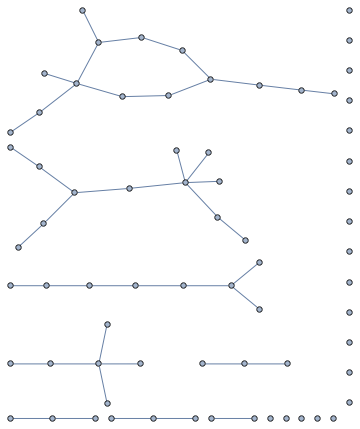
\includegraphics[width=1\linewidth]{erdos-renyi/G(70,0'02).png}
		\caption{$G(70,0.02)$}
		\label{fig:K16}
	\end{subfigure}
\begin{subfigure}{.5\textwidth}
	\centering
	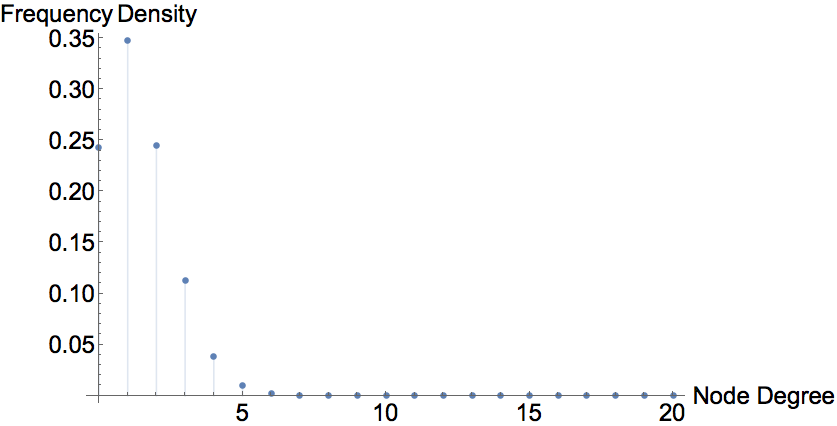
\includegraphics[width=1\linewidth]{erdos-renyi/e-r-prob-dist-3.png}
	\caption{$G(70,0.02)$}
	\label{fig:K16}
\end{subfigure}
	\caption{Examples of Erd\H{o}s-R{\'e}nyi graphs on the left with the expected probability distributions of Erd\H{o}s-R{\'e}nyi graphs with these parameters.}
	\label{fig:erdos-renyi-graphs}
\end{figure}
%\paragraph{Limitations}
Unfortunately $G(n,p)$ has two major limitations in modelling real-world social networks: it has an unrealistic degree distribution and it has low clustering.\\
\\
%\paragraph{Degree Distribution}
Firstly, the degree distribution of $G(n,p)$ is a binomial distribution. That is to say the probability of a node being connected to $k$ others is:
\begin{equation}
	p_k=\binom{n-1}{k}p^k(1-p)^{n-1-k}
\end{equation}
This is easily understood. Each node can be connected to $n-1$ others, there are $\binom{n-1}{k}$ ways to be connected to $k$ of them, and the probability of having exactly $k$ edges is $p^k(1-p)^{n-1-k}$. This means that the degree of the vertices has the binomial distribution $B(n-1,p)$. However, the binomial distribution does not have `heavy tails', a feature often found in real-world networks including social networks\cite{barabasi-albert}. This limits the ability of $G(n,p)$ to model social networks.\\
\\
It is worth explaining the meaning of `heavy-tailed'. Qualitatively this means that in a sample from a heavy-tailed distribution you are more likely to get a small number of very high values. Quantitatively it means that the right tail of the distribution has a heavier tail than the exponential distribution\cite{heavy-tailed}. That means that the probability distribution function has higher values for large $x$ (Figure \ref{fig:heavy-tailed}).
\begin{figure}
	\centering
	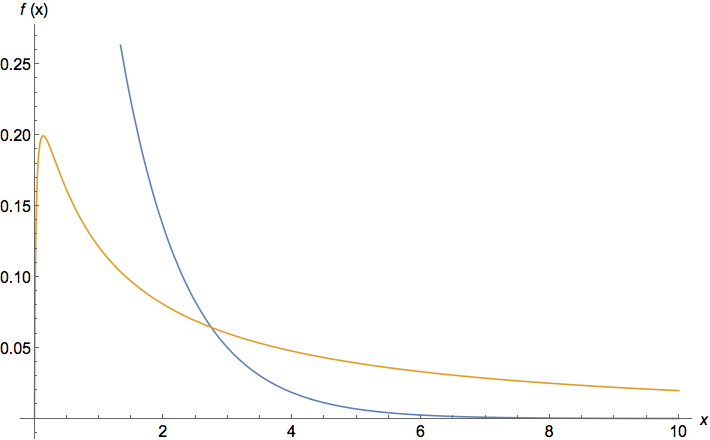
\includegraphics[width=.9\linewidth]{erdos-renyi/heavy-tailed.png}
	\caption{A graph showing the pdf of the exponential distribution in blue against the `heavy-tailed' log-normal distribution in orange.}
	\label{fig:heavy-tailed}
\end{figure}
%\textit{Mark: say something about what it means to be heavy-tailed}
\label{mmd}
\\
\\
%\paragraph{Clustering}
Secondly, $G(n,p)$ does not show nodes clustering as much as a real-world network. The clustering coefficient, $C$ is a measure of how likely nodes are to be in clusters. Formally, it is the probability that two neighbours of a vertex are also neighbours of each other\cite{networks}. In the Erd\H{o}s-R{\'e}nyi graph, this probability is independent of all other edges. Hence the expectation of the clustering coefficient is simply $\langle C\rangle=p$.\\
\\
This says that two neighbours are just as likely to be connected if they have a neighbour in common as if they do not. Most real social networks have high clustering, resulting from a phenomena called triadic closure\cite{simmel}\cite{strength-weak}. This just means that two of your friends are more likely to know each other than two random people. To see this, think of all your mutual friends and also how you tend to meet your friend's friends eventually.\\
\\
%\subsubsection{Summary}
Whilst the Erd\H{o}s-R{\'e}nyi graph does not provide an accurate representation of most social networks, its simplicity makes it useful for running some models. However, we will also consider some graphs that avoid the problems faced by the Erd\H{o}s-R{\'e}nyi graph.
\subsubsection{Scale-free graphs: the Barab\'asi-Albert model}
Scale-free graphs are defined as graphs that have distributions of node degree that follow a power law. That is the probability of a node being connected to exactly $k$ others is $p_k\sim k^{-\gamma}$ where $\gamma>0$. Early promoters of scale-free networks claim that they are prevalent throughout real-world networks\cite{barabasi-albert}. However, recent reviews of large datasets suggest that there is limited evidence for this\cite{scale-free-rare}.\\
%\\
%\textit{Say what scale-free means here}
\label{mmd}
%\\
\\
Regardless, the Barab\'asi-Albert model is one of the most widely known models that can generate scale-free networks. It does so by generating graphs by a process of \textit{preferential attachment}\cite{barabasi-albert}. 
\begin{figure}
	\centering
	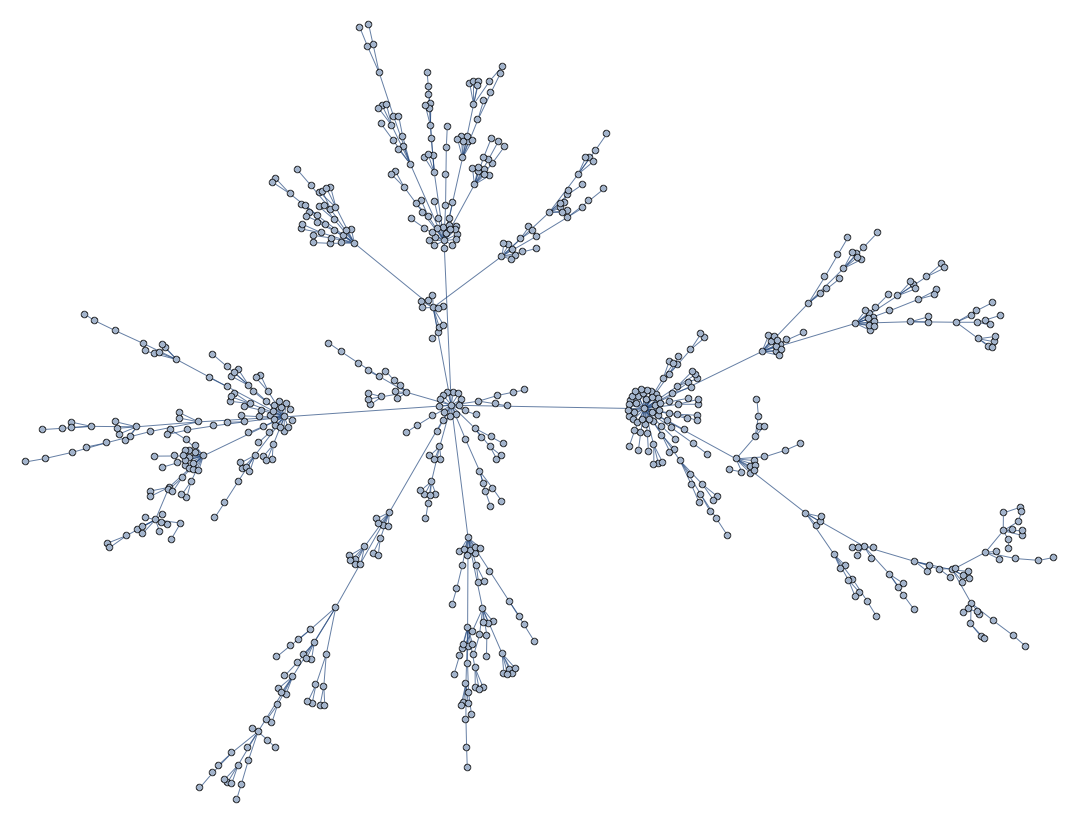
\includegraphics[width=.9\linewidth]{barabasi-albert/700.png}
	\caption{A graph with 700 nodes created from the Barab\'asi-Albert model}
	\label{fig:ba-700}
\end{figure}
%\paragraph{Setup}
A Barab\'asi-Albert graph is made by the following process. Start with a graph of two connected nodes. We take discrete steps in time and at each step we add one node and connect it to one existing node. The existing node is chosen with probability proportional to its degree. That is, a node with degree $k$ is $k/l$ times more likely to connect to  than a node with degree $l$\cite{galla}.\\
\\
%\paragraph{Properties}
This preferential attachment results in a graph with a heavy-tailed distribution in which there are a few highly connected `super-nodes' and many nodes with only a few connections. This is similar to real-world networks. We can find the probability distribution of the node degree. Using a master equation method that describes the evolution of the graph, we can derive that $p_k\sim k^{-3}$\cite{galla}. This confirms that the distribution is roughly the right shape. 
\\
\\
%\paragraph{Limitations}
Whilst the Barab\'asi-Albert model produces a reasonable degree distribution, it fails to give a clustering coefficient as high as those in social networks\footnote{Whilst there are simpler heuristic estimates of the exact clustering coefficient, the exact analytic value is $\frac{m-1}{8}\frac{(\log n)^2}{n}$\cite{ba-cluster}}. This motivates the development of another graph model.
\subsubsection{Small-world graphs: the Watts-Strogatz model}
The Watts-Strogatz Model avoids this shortcoming and captures the property of many real networks of having both high clustering and short path lengths\cite{watts-strogatz}. A graph having short path lengths means that there is a short path between any two nodes in a connected component. This gives the Watts-Strogatz its alternative name of the `small-world model'.
\begin{figure}
	\centering
	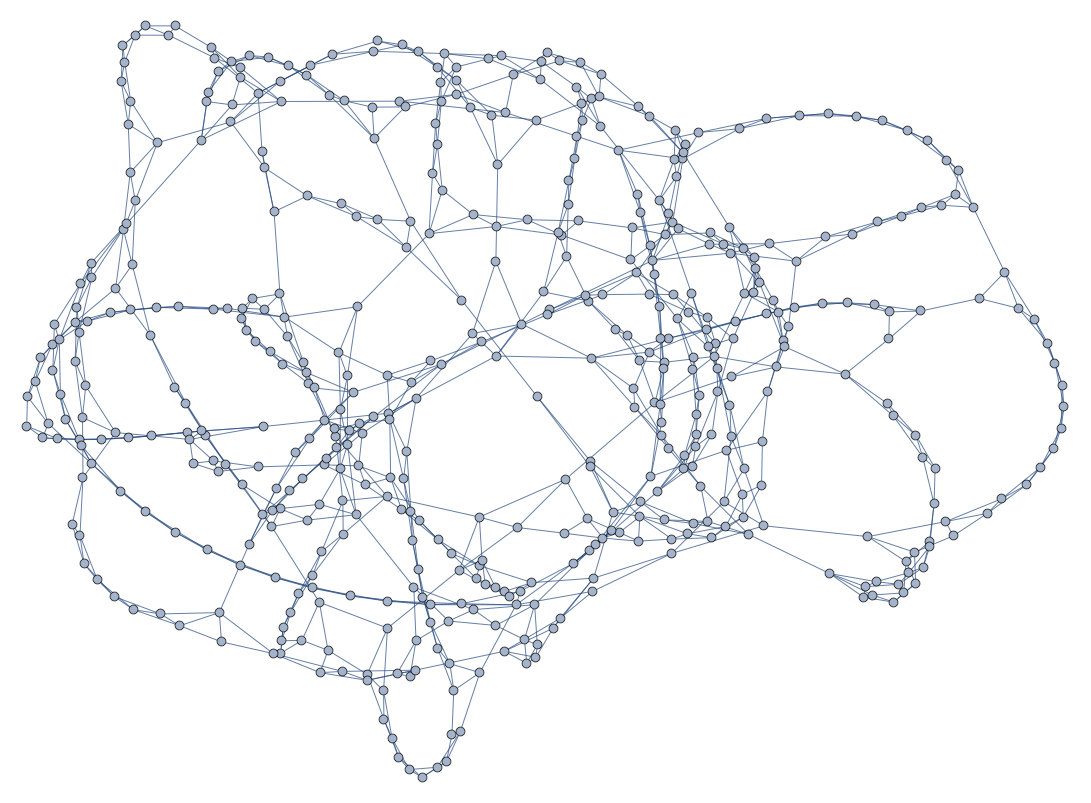
\includegraphics[width=1\linewidth]{watts-strogatz/500,0`5.png}
	\caption{A graph of 500 nodes created from the Watts-Strogatz model with a rewiring probability $0.5$}
	\label{fig:ba-700}
\end{figure}
\\
\\
The Watts-Strogatz model is constructed in two parts.
\begin{enumerate}[nosep]
	\item\label{w-s-1} \textit{Make a ring lattice} Take $n$ nodes. These are each given a number $i$. Then the $i^{\text{th}}$ node is connected to $K/2$ nodes below it and $K/2$ nodes above it, modulo $n$. 
	\item\label{w-s-2} \textit{Rewire} Then after this, for each pair of nodes, rewire them with probability $\beta$. To rewire an edge means to remove that edge and replace it with another that avoids loops or parallel edges.\\
\end{enumerate}
Step \ref{w-s-1} creates the high clustering and the random links introduced in step \ref{w-s-2} give the short average path lengths. The parameter $\beta$ mediates between these two characteristics. Indeed in the limit $\beta=1$, it approximates an Erd\H{o}s-R{\'e}nyi graph which as we've seen has low clustering. In the limit $\beta=0$ it is a ring lattice which has long average path lengths.\\
\\
However, it now fails where the Barab\'asi-Albert graphs succeeded in that its probability distribution is not as long-tailed as a real-network. Hence choosing between these two graphs is a trade-off. In practice the best choice depends on what features one is investigating.
%\subsubsection{Exponential Random Graphs}
%-- Wait for Data Science Institute talk on this next week --
\subsection{Real-world network datasets}
An alternative to using a random graph is to use a real-world dataset. For example, Facebook have access to a dataset of the social network of almost 2 billion people\cite{num-fb-users}. Whilst researcher's access to this data is becoming rapidly more limited due to very valid privacy concerns it is still easy to obtain a subset of this data by `scraping' the friends list of public profiles, as seen in Figure \ref{fig:facebook-network}. This has the problem that there are people who are not on Facebook and also that many users do not have their friend lists accessible to the public. A readily available and anonymised set of data can be found online\cite{fb-ego-data}. This is a graph of $4039$ nodes and $88234$ edges.\\
\\
Currently the largest open-source dataset of a social network is a dataset of the Friendster network\cite{friendster-data-archive}. This graph dwarfs the pre-organised Facebook data, containing $117,751,379$ nodes and $2,586,147,869$ directed edges. A slightly tamed version exists \cite{friendster-data-stanford} that takes the induced subgraph of users who are have at least some connection to the rest of the community, ignoring the stand-alone users. Whilst this is too large and unwieldy for this paper, a more manageable dataset could be attained by choosing a node and considering the induced graph of all nodes within a path of length, say, three from this node.\\
\\
For specific problems it may be worth conducting data gathering missions to map specific networks. For example sometimes research is done on specific communities such as the social networks of autistic school children\cite{anderson_locke_kretzmann_kasari_2015} or the relationships between Chilean astronomers\cite{chilean-astronomers}. The benefits of using datasets are that we know that the networks we are simulating on relate to some real-world network. This means we have some guarantee that it at least looks a bit like the underlying network we are trying to model.\\
\\
The negatives of this route are that it is just one instance of a network. It seems like, for example, the Facebook friendship network \textit{could} have looked differently but kept similar features. One way to deal with this shortcoming is by using exponential random graphs. This is a family of random graphs whose probability distribution is designed to make it highly likely that a graph drawn from this distribution shares certain key properties such as mean degree or degree distribution\cite{networks}. This feature has made them of use in modelling social networks\cite{exponential-random-graph}.
%\textit{Mark: I’d say something like “this is a family of random graphs whose probability distribution is designed to make it highly likely that a graph drawn from the distribution shares certain key properties—mean degree, or degree distribution—}
\label{mm}
%This is a family of random graphs that are generated in such a way that it makes it highly likely the a are graphs that can take the properties of the specific instance of the graph to created many more with the same properties\cite{networks}.
Another, less avoidable, problem is that network data that serves as a proxy or approximation for a real underlying data will often be incomplete, particularly if the dataset is large and automatically collected such as the Facebook or Friendster data.
\subsection{Example: Boltzmann wealth model on a network}
So far we have developed a model of the transfer of wealth that assumed that relationships between agents are homogeneous. That is, they can transfer money with every agent equally easily. We can think of the agents as nodes and the ability to transfer wealth between two agents as an edge. Then the model we were previously using is the equivalent of a complete graph, the graph in which each node is joined by an edge to every other\footnote{See Chapter \ref{ch:games-on-networks} for a primer on graph theory.}.\\
\\
As explored in the previous section, many real situations are not as homogeneous as this. Therefore it makes sense to consider cases in which some agents cannot transfer to others. To do this in an ABM we keep the agents the same but change the environment in which they exist and the rules they interact by.
\subsubsection{On a 2D Lattice}
One interesting thing to do is to make the environment a 2-dimensional lattice which the agents can move on. Then the nodes of the graph do not represent individual agents but spaces in which the agents can inhabit. That is we consider each agent as being at a certain position on a 2D lattice. We can add some rules to the Boltzmann wealth model to do this:
\begin{enumerate}[
%	label={Rule \arabic*}
	]
	\setcounter{enumi}{\value{rule}}
	\item At each tick, an agent moves to a neighbouring square.
	\item Multiple occupancy is allowed
	\item An agent can transfer money to any agent on a neighbouring square, including on their own square
\end{enumerate}
Implementing this requires that the individuals store two extra parameters: x and y position. They also need a method to allow them to both move position and check the position of other agents to see if they are neighbours.\\
\\
Implementing this on a 2D lattice with the Moore neighbourhood gives a new model with different dynamics. Running this program with 100 agents on a $10\times10$ grid and plotting the result after 100 ticks gives figure \ref{fig:space-1}. The graph shows the wealthiest agent in that square. Interestingly the wealthiest agents with $3$ or $4$ units of wealth are usually surrounded by a high proportion of agents with $0$ units of wealth.
\begin{figure}[!h]
	\centering
	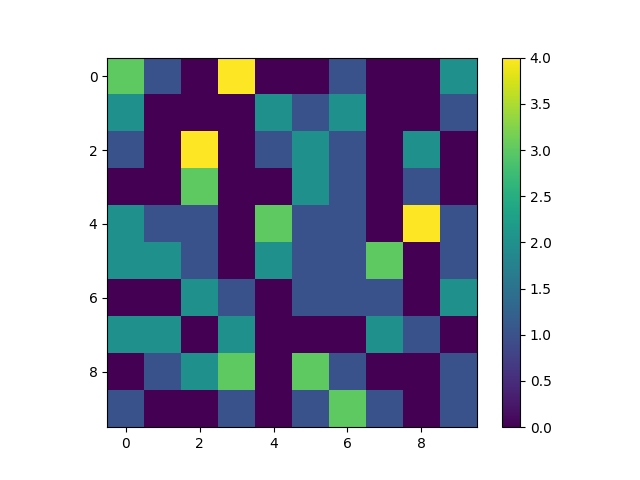
\includegraphics[width=.9\linewidth]{boltzmann-wealth/space-1.png}
	\caption{The Boltzmann wealth model on a 2D lattice. The grid on the left is the 2D lattice with the colours representing the wealth of the wealthiest agent in that square. Specifically yellow represents a wealth of $4$ and the dark blue a wealth of $0$.}
	\label{fig:space-1}
\end{figure}
\subsubsection{On an Barab\'asi-Albert network}
We can also consider the same basic model but on other types of network. Moving back to the assumption that  the agents are fixed in their neighbours and do not move, we let each agent be a node in the network. Running the simulation on a Barab\'asi-Albert network provides an interesting augmentation of the original model.\\
\\
We choose to perform 100 runs of this simulation with $50$ agents on an Barab\'asi-Albert network. Plotting the same graph of frequency density of wealth shows that the network simply amplifies the inequality we saw previously (Figure \ref{fig:network-ba-1}).
\begin{figure}[!h]
	\centering
	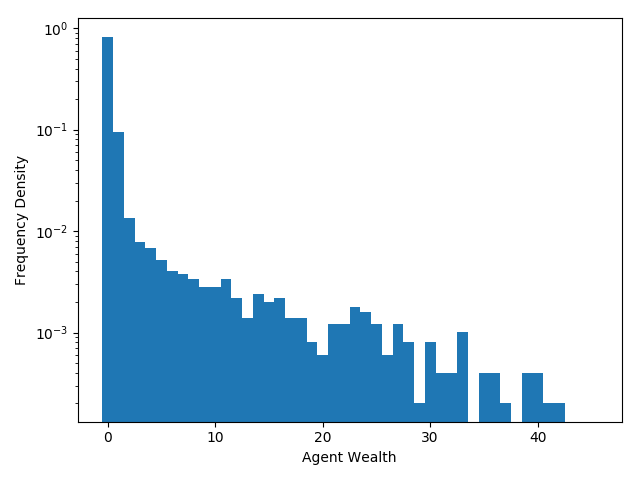
\includegraphics[width=.9\linewidth]{boltzmann-wealth/network-ba-1-log.png}
	\caption{Boltzmann wealth model on a Barab\'asi-Albert network. The resulting wealth inequality is so severe that the graph has to be plotted with a log scale on the y-axis. Around 80\% of the population have a wealth of $0$ while there are individuals with wealths of $40$.}
	\label{fig:network-ba-1}
\end{figure}
If we look in more detail we can see that the wealth of an agent is positively correlated to the degree of the node (Figure \ref{fig:network-ba-cor}). Now over $80\%$ of the population has $0$ units of wealth and some agents end runs with over $40$ units, constituting $80\%$ of the total wealth in their population.
\begin{figure}[h]
	\centering
	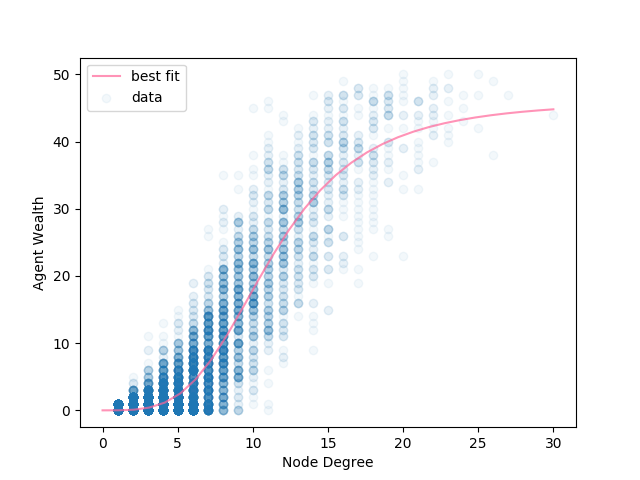
\includegraphics[width=.9\linewidth]{boltzmann-wealth/network-ba-cor2.png}
	\caption{Correlation between node degree and wealth in the Boltzmann wealth model on the Barab\'asi-Albert network. Each point represents the node degree of an agent and its wealth at the end of a run. This plot shows the result of 1000 runs each time running with 50 agents for 100 steps. The data is fit with a sigmoidal curve of best fit.}
	\label{fig:network-ba-cor}
\end{figure}

%Could say something about measures of gini
%To summarise, changing the underlying network of a model can have a major effect on the dynamics.
\section{Converting deterministic epidemiological models to ABMs}
We have learnt how ABMs can work, typical ways of analysing them and how the underlying network can affect the dynamics. With this we can move back towards studying epidemiology and revolutions. The first step we can make is to adapt the ideas from the deterministic compartmental models in Chapter \ref{ch:compartments} to an agent-based model on a network that can incorporate discreteness and stochasticity.
\subsection{Stochastic SIR model}
\subsubsection{Building the model}
%put on graph
We will start by adapting the simplest SIR compartmental model to make an ABM. The first step is to make the agents discrete. To do this we represent each agent as a node, creating $n$ nodes. We then have some edges joining them. We don't need to define the edges yet but we know that in general they join some nodes and not others. These edges together with the nodes form a graph $G$.\\
\\
%states and moving between states: infective to removed
The next step is to adapt the properties of classes in the population to properties of each agent. For example, instead of a class's size decreasing by a certain rate, we want each individual in that state to have a certain probability of moving to another state in any time. Previously we had three classes. To adopt this we have three states agents can be in: susceptible, infected and removed. Before we had that the infective class decreases at a rate of of $\alpha I$ whilst the infective class increases at the same rate. To adopt this we have that each individual moves from infective to removed with rate $\alpha$.\\
\\
%moving between states: susceptible to infective
Reinterpreting the movement from susceptible to infected takes a bit more thought. Previously to define the rate of contacts we assumed the law of mass action. However as we will incorporate a network structure for the environment, we are looking for something more sophisticated than this. Specifically we want to represent that some agents are more likely to come into contact than others.\\
\\
To do this it helps to break down the meaning of the contact rate $\beta$ from chapter \ref{ch:compartments}. Technically $\beta$ is the product of two parameters: the probability of contact between two individuals, $p$, and the probability of a contact leading to infection, $c$. In the previous compartmental model through the assumption of mass action we assumed that the probability of contact between any two individuals, $p$, was equal. However on a general network this is not true.\\
\\
Now we have $p=0$ for any non-neighbours and $p\neq0$ for neighbours. It makes intuitive sense for $c$ to be constant for any disease regardless of the model we are using. Therefore to make the values of $\beta$ we use comparable between the compartmental and agent-based models we need to adjust the value of $p$. Define $\hat n$ to be the average number of neighbours a node has. Let $\hat p$ be the probability of contact between two individuals in the network model. Then we need $\hat n \hat p = p N$. This ends up making the contact rate in the ABM $\hat\beta=\beta N/\hat n$.\\
%\\
%\textit{Mark: I see what you mean about this section. Do you have a clearer idea of what you want to say now?}
\label{mmd}
\\
Finally, mirroring the initial conditions we set just a single node as infective.\\
\\
We can summarise all of this succinctly:
\begin{enumerate}[nosep]
	\item There is a graph of $n$ nodes where each node is an individual
	\item The individual can be in one of three states: susceptible, infective or removed
	\item Two neighbouring individuals come into contact at a rate $p$. This contact rate is independent of the degrees of the two nodes.
%	\textit{Mark: Is this contact rate independent of the degrees (or number of neighbours) of the  two nodes?}
	\label{mmd}
	\item An infective infects a susceptible upon contact with probability $c$, after which the susceptible becomes infective
	\item Infectives are removed at a rate $\alpha$
	\item Initially there is a single node that is infective	
\end{enumerate}
\subsubsection{Running the simulation}
To support the agent-based modelling, the code uses the MESA framework. This is an open-source modular framework that aims to aid research in modelling, analysing and visualising agent-based systems in Python\cite{mesa-github}. Using MESA we can create an interactive sandpit for experimenting with different parameter values on this model (Figure \ref{fig:SIR-interactive}).
\begin{figure}[h]
	\centering
	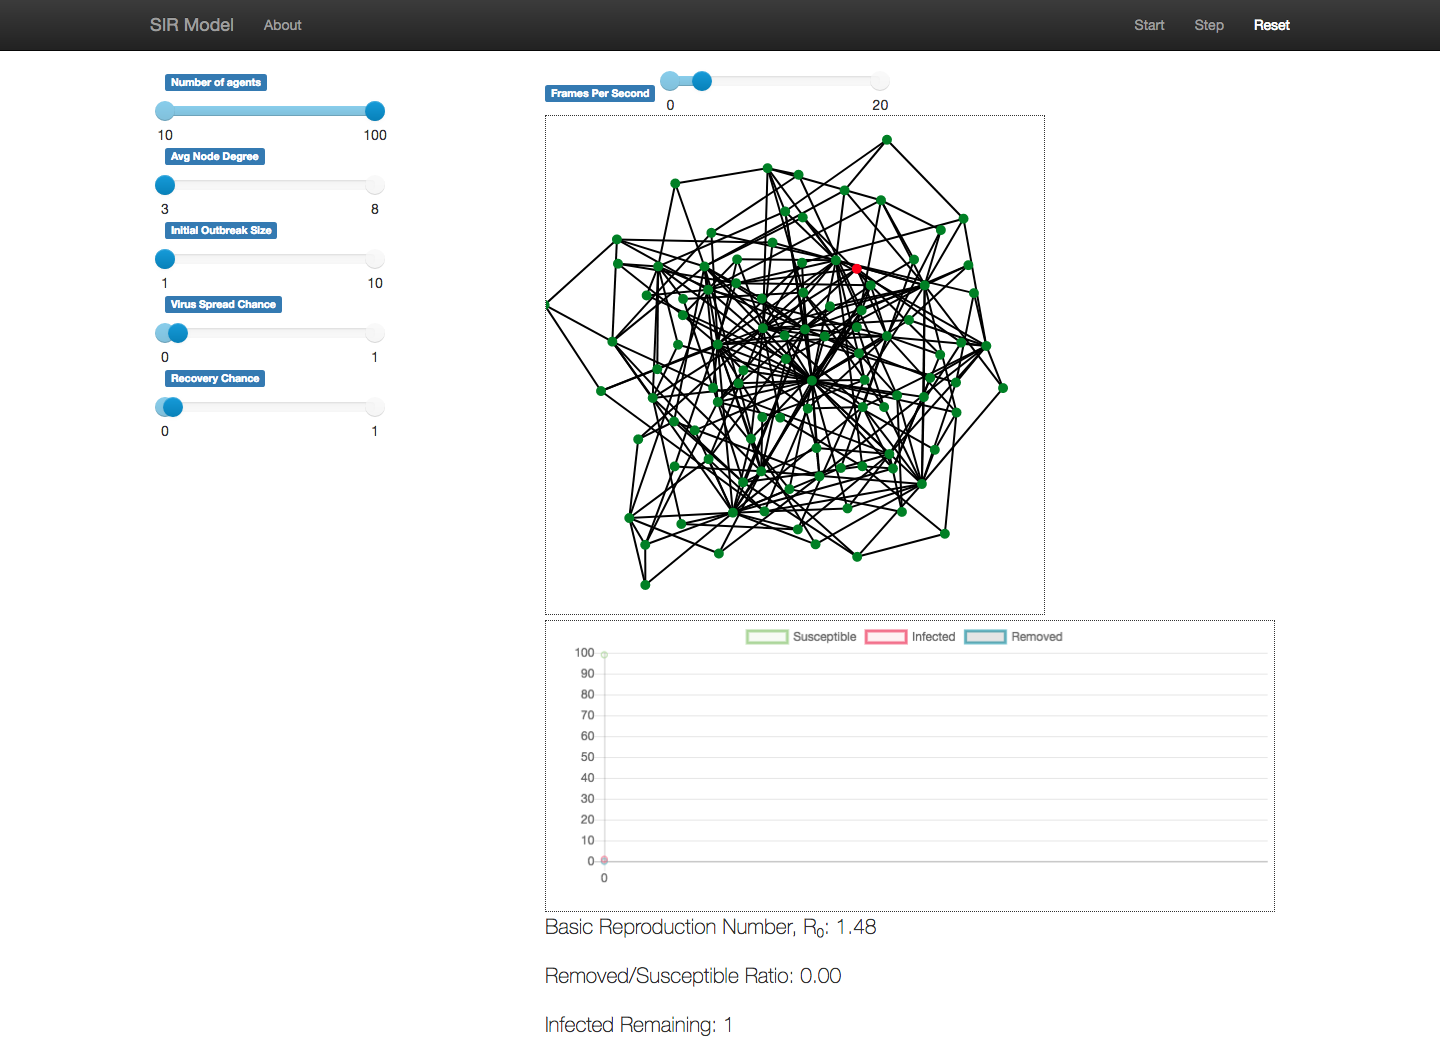
\includegraphics[width=\linewidth]{SIR-network/SIR-interactive.png}
	\caption{The interactive screen of the SIR model. We have a similar screen for all following ABMs. On the left we can adjust parameter values, in the centre there is a live view of the dynamic network, below that an updating graph of class size against time and at the bottom we have some key statistics such as the value of $R_0$. The top bar allows the user to stop and start the simulation as well as find out further information about the model.}
	\label{fig:SIR-interactive}
\end{figure}
\begin{figure}
	\centering
	\begin{subfigure}{.3\textwidth}
		\centering
		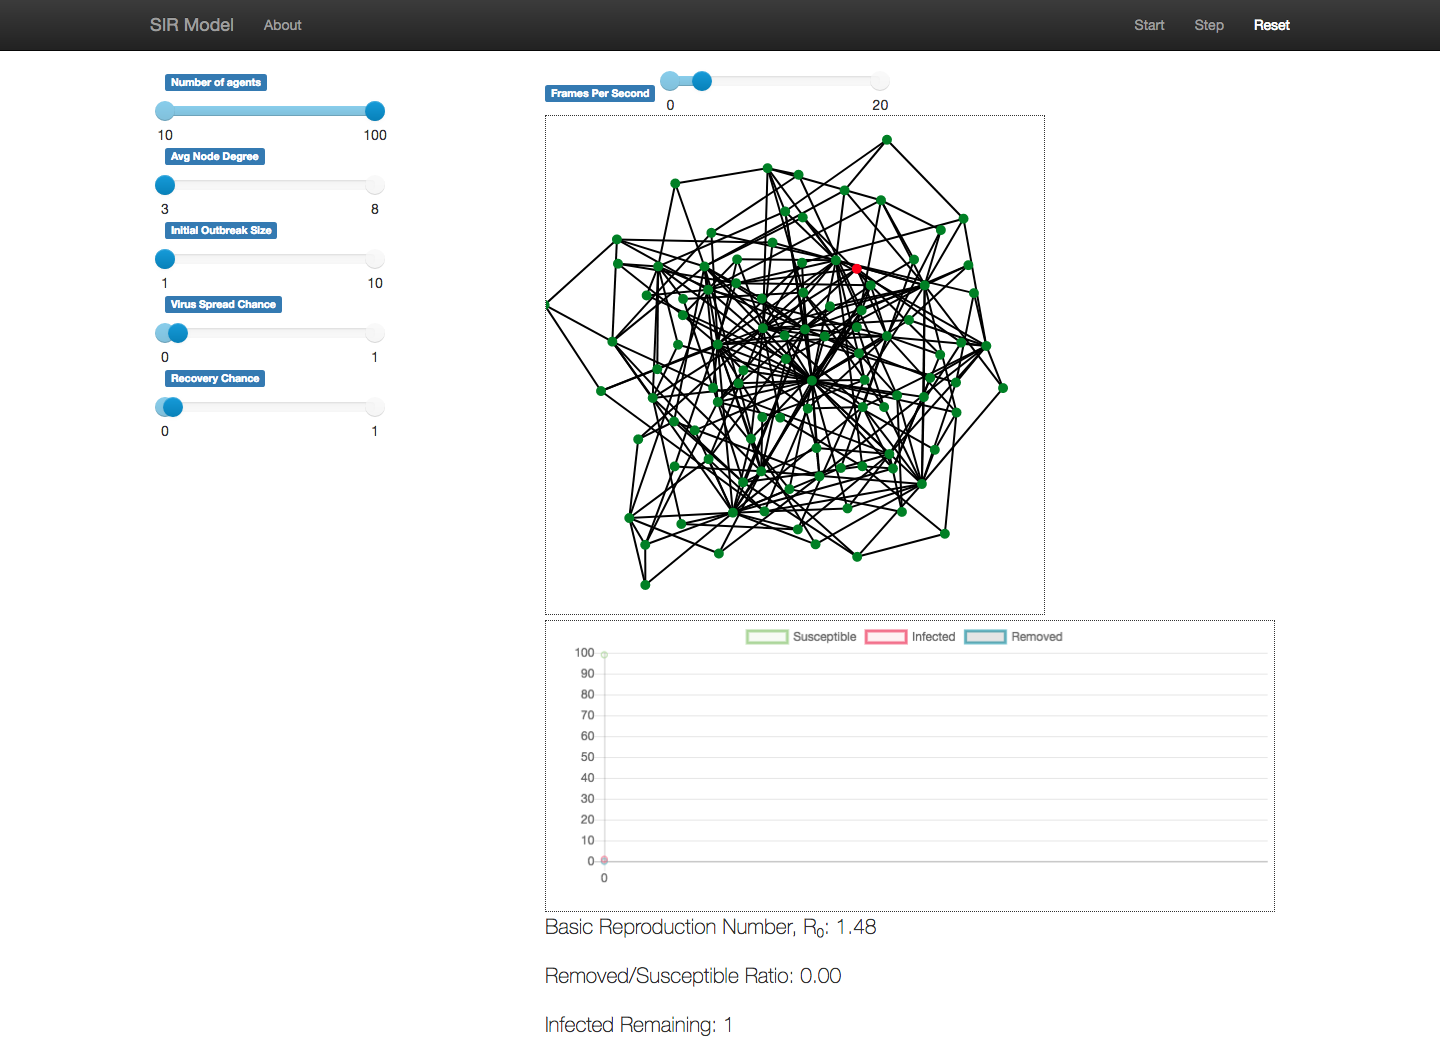
\includegraphics[width=1\linewidth,trim={19.275cm 16cm 14cm 4.5cm},clip]{SIR-network/SIR-interactive.png}
		\caption{$t=0$}
		\label{fig:SIR-network-1}
	\end{subfigure}%
\begin{subfigure}{.3\textwidth}
	\centering
	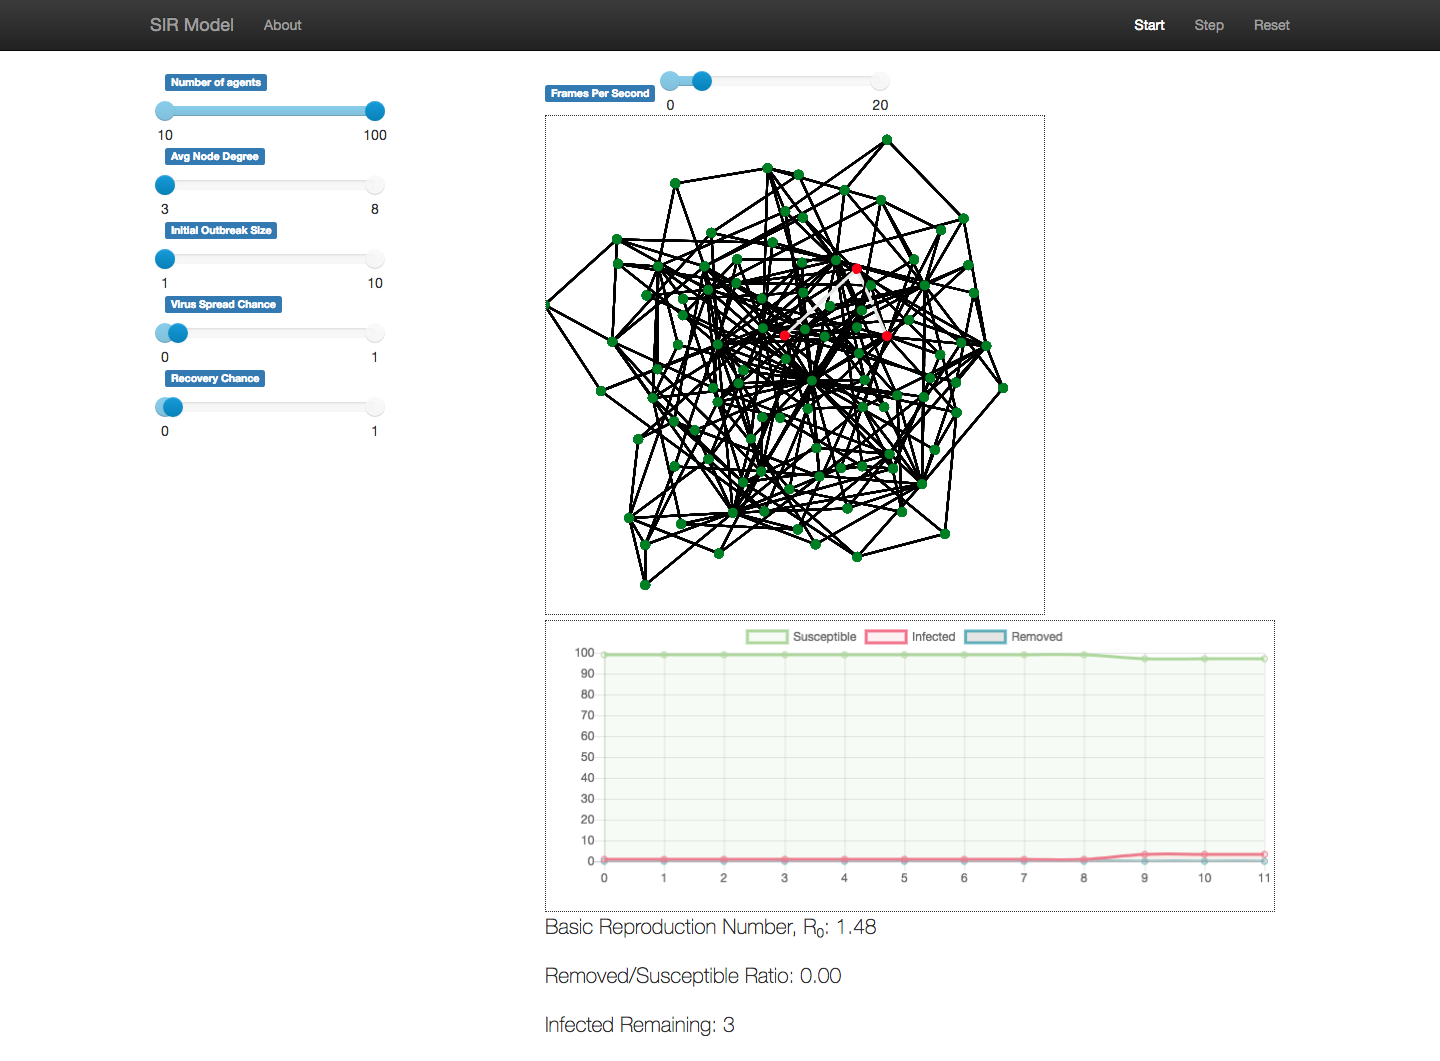
\includegraphics[width=1\linewidth,trim={19.275cm 16cm 14cm 4.5cm},clip]{SIR-network/SIR-interactive-2.png}
	\caption{$t=15$}
	\label{fig:SIR-network-2}
\end{subfigure}%
	\begin{subfigure}{.3\textwidth}
		\centering
		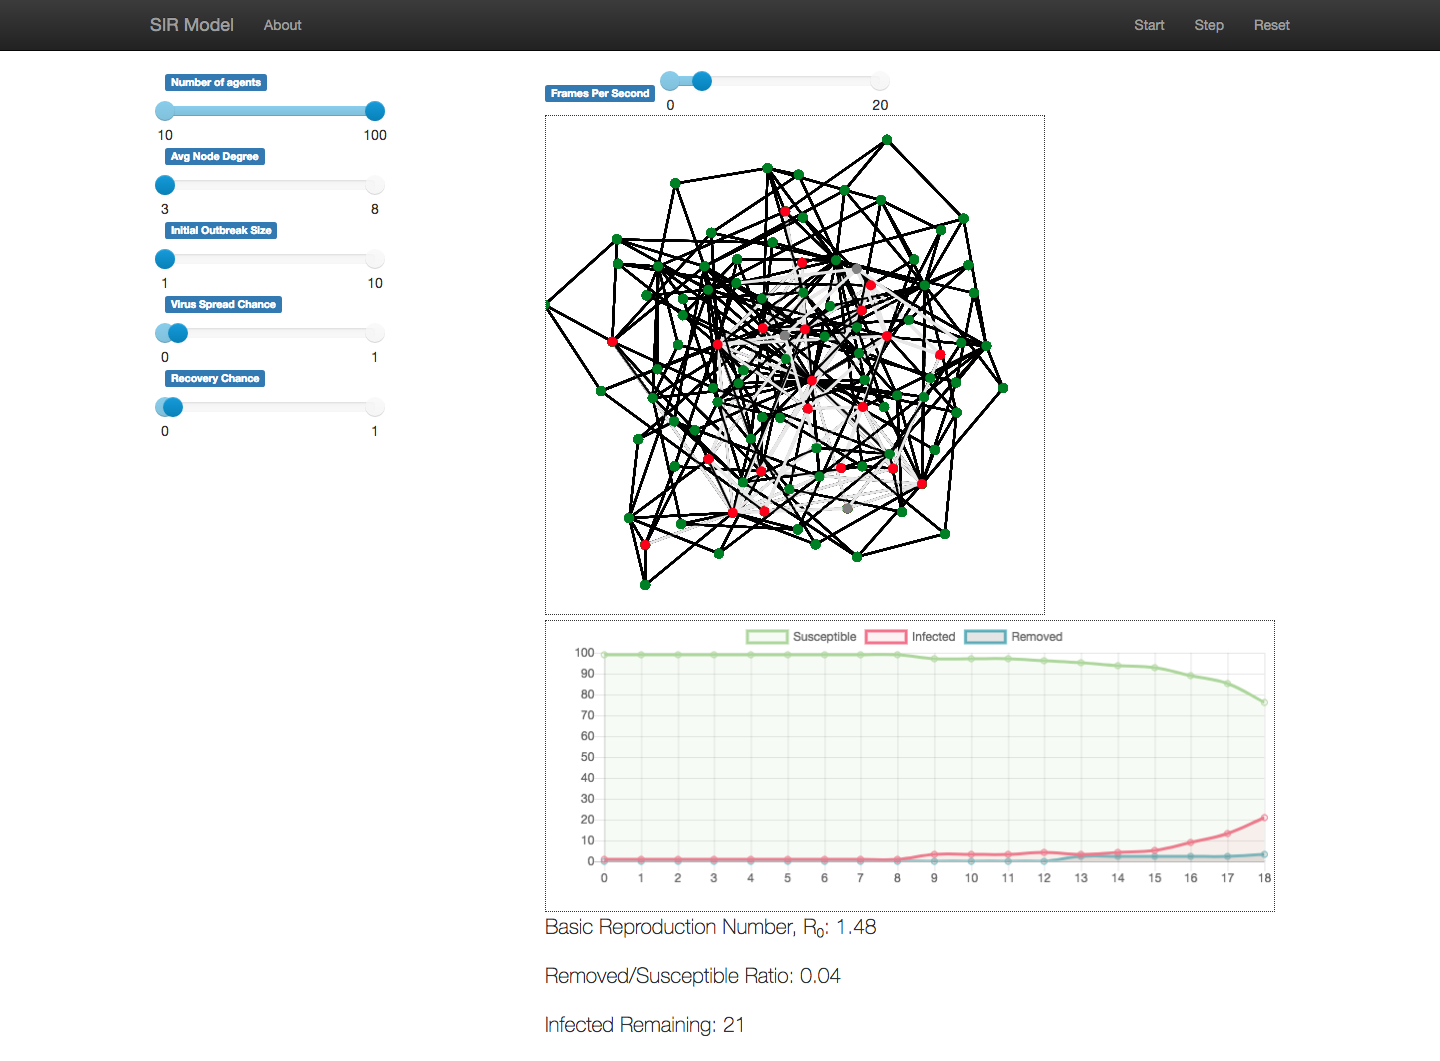
\includegraphics[width=1\linewidth,trim={19.275cm 16cm 14cm 4.5cm},clip]{SIR-network/SIR-interactive-3.png}
		\caption{$t=30$}
		\label{fig:SIR-network-3}
	\end{subfigure}
	\caption{The evolving network in the agent-based SIR model with $70$ nodes. Green, red and grey dots represent susceptible, infective and removed individuals respectively. Black edges represent that the infection could still be passed through that edge whilst grey edges mean that neither of the two nodes are susceptible.}
	\label{fig:SIR-network-run}
\end{figure}
\\
\\
We start by running a simulation with a small number of individuals (Figure \ref{fig:SIR-network-run}). We can see that this new model can reflect the fact that the growth of classes is stochastic, going both up and down, such as at the peak of the infective class's size in Figure \ref{fig:SIR-graph-1}.
\begin{figure}[h!]
	\centering
	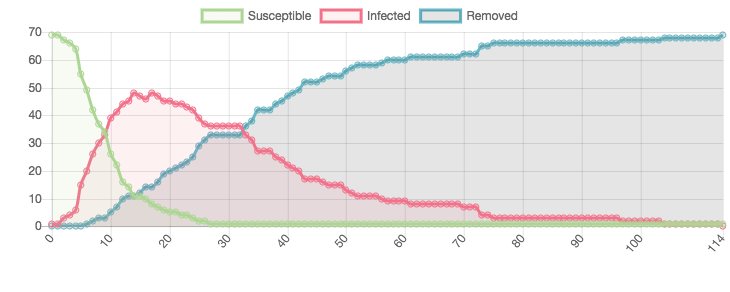
\includegraphics[width=\linewidth]{SIR-network/1.png}
	\caption{A graph of the change in the three classes size through time in the agent-based SIR model with $70$ nodes.}
	\label{fig:SIR-graph-1}
\end{figure}\\
\\
With a higher number of individuals, if the revolution gets going we see that it is very smooth due to the law of large numbers (Figure \ref{fig:SIR-graph-2}). In this case we can see that the dynamics approximate the dynamics seen in the continuous compartmental models which is reassuring.
\begin{figure}[h!]
	\centering
	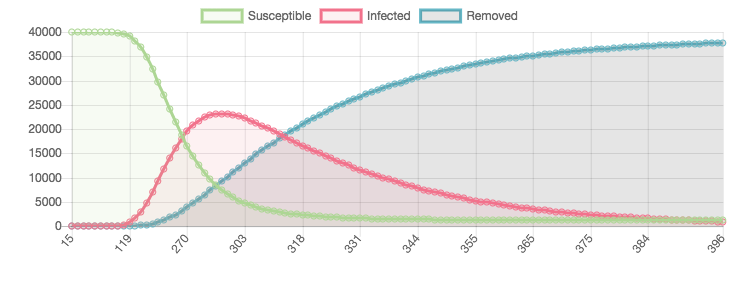
\includegraphics[width=\linewidth]{SIR-network/2.png}
	\caption{The SIR ABM with $40000$ agents.}
	\label{fig:SIR-graph-2}
\end{figure}\\
\\
The important distinction between the compartmental model and the ABM is that now the infection can die out even with $R_0>1$.
\begin{figure}[h!]
	\centering
	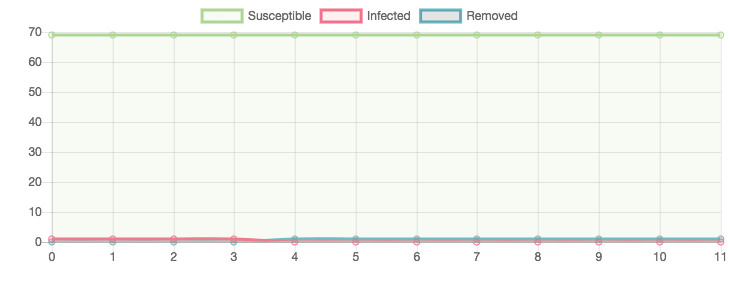
\includegraphics[width=\linewidth]{SIR-network/3.png}
	\caption{An infection dying out on the SIR model even with $R_0=1.07>1$}
	\label{fig:SIR-graph-3}
\end{figure}
The probability that the infection dies with the first infective is $\beta\hat n/(\alpha+\beta\hat n)$. This is because the time it takes on average for an infective to infect a susceptible is exponentially distributed with parameter $\beta \hat n$ where $\hat n$ is the average number of neighbours a node has. Also the time it takes for an infective to be removed is exponentially distributed with parameter $\alpha$. So the probability that the infection will run out in the early stages is $>\beta\hat n/(\alpha+\beta\hat n)$.
\subsection{Stochastic SEIR model}
Next, as before, we introduce the exposed class. Exposed nodes become active at a rate of $\gamma$ and active nodes are removed at a rate of $\alpha$. The mechanism for moving from susceptible to active now describes the move from susceptible to exposed. Again putting all of the rules in a list and using italics to highlight the rules that differ from the SIR model:
\begin{enumerate}[nosep]
	\item There is a graph of $n$ nodes where each node is an individual
	\item The individual can be in one of \textit{four} states: susceptible, \textit{exposed}, infective or removed
	\item Two neighbouring individuals come into contact at a rate $p$
	\item An infective infects a susceptible upon contact with probability $c$, after which the susceptible becomes \textit{exposed}
	\item \textit{Exposed individuals become infective at a rate $\gamma$}
	\item Infectives are removed at a rate $\alpha$
	\item Initially there is a single node that is infective
\end{enumerate}
\bigskip
Running this we see, as in the compartmental SEIR model that the introduction of the exposed class dampens the rate of increase in the infected population (Figure \ref{fig:SEIR-network-1}).
\begin{figure}[h!]
	\centering
	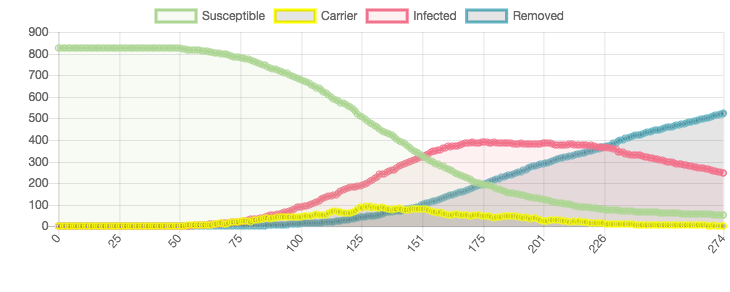
\includegraphics[width=\linewidth]{SEIR-network/1.png}
	\caption{}
	\label{fig:SEIR-network-1}
\end{figure}
Also because of the stochastic elements the model permits wipe-out even with $R_0>1$.
\subsection{Stochastic agent-based revolution model}\label{sec:abm-rev}
Now we can fully describe and implement a stochastic agent-based model of a revolution on a network.\\
\\
The movements from $S\rightarrow E$, $I\rightarrow R$ are the same as described in the SEIR model. However we need to incorporate a version of the non-linear movement from $E\rightarrow I$ that we devised in section \ref{sssec:zealots}. The part we need to adapt is the threshold $k$ for social influence. In the compartmental model of revolution $k$ was a fraction of the population which represented the threshold for non-zealots to become involved in a revolution. However, one of the key benefits of simulating on a network is that we do not assume each individual has an omniscient view of the population. Instead their view is highly localised and limited to their neighbours on the graph. So instead of a proportion of the population we want $k$ to represent a threshold for how many neighbours need to be active for an individual to become active. That is, the value given will be the number of active neighbours, $\hat i$, an exposed individual has to have for them to turn their idea into action. Based on the research we justified our previous decision with, this is around $3$ people\cite{asch-conformity}. So we now set $\hat k=3$. Then an exposed individual moves to active with probability
\begin{equation}\label{eq:non-zealot-abm}
\gamma \frac{\hat i^n}{k^n+\hat i^n}
\end{equation}
Further we give every agent an attribute: zealot or non-zealot. This determines if they will move to the active state when exposed with rate given by equation \ref{eq:non-zealot-abm} or the zealot rate $\delta$. This is a property held all the time by all agents and does not change. However it only affects their transition rate $E\rightarrow I$.\\
\\
Written out these rules are:
\begin{enumerate}[nosep]
	\item There is a graph of $n$ nodes where each node is an individual
	\item The individual can be in one of four states: susceptible, exposed, infective or removed
	\item \textit{Each individual is of one of two types: zealot or non-zealot}
	\item Two neighbouring individuals come into contact at a rate $p$
	\item An infective infects a susceptible upon contact with probability $c$, after which the susceptible becomes exposed
	\item \textit{If an exposed individual is a zealot, they become infective at a rate $\gamma \frac{\hat i}{k^n+\hat i^n}$}
	\item \textit{Otherwise if an exposed individual is a non-zealot they become infective at a rate $\delta$}
	\item Infectives are removed at a rate $\alpha$
	\item Initially there is a single node that is infective
\end{enumerate}
\bigskip
We choose to first run this model on a Watts-Strogatz network with 70 nodes (\ref{fig:abm-rev-70}). 
\begin{figure}[h]
	\centering
	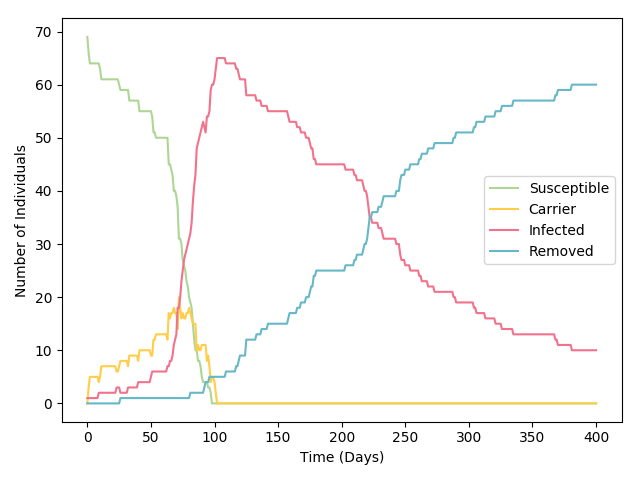
\includegraphics[width=\linewidth]{rev-abm/rev-ws.png}
	\caption{A typical trajectory using default parameters on a Watts-Strogatz network with $70$ agents.}
	\label{fig:abm-rev-70}
\end{figure}
Making the number of nodes much larger confirms that the model shares many qualitative properties with the previous compartmental model of Section \ref{sec:rev-compartment}.
\begin{figure}[h]
	\centering
	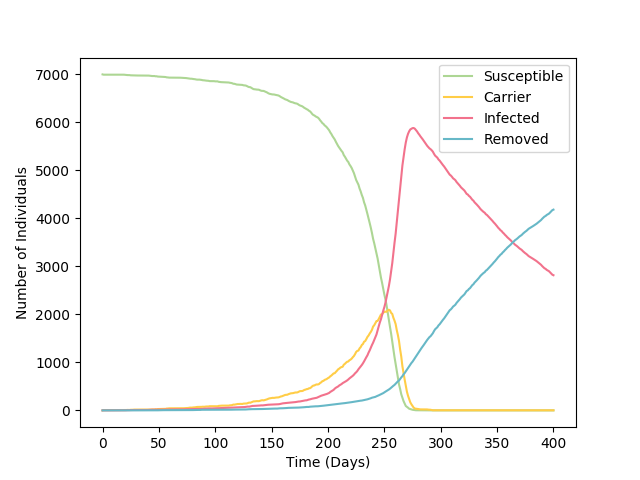
\includegraphics[width=\linewidth]{rev-abm/rev-abm-2.png}
	\caption{A typical trajectory using default parameters on a Watts-Strogatz network with $7000$ agents}
	\label{fig:abm-rev-7000}
\end{figure}
Again, importantly the model allows the possibility of the growth of the infective class ending prematurely even with $R_0>1$ meaning it does not follow the same qualitative pattern as the compartmental model. Whilst this is an obvious strength, there are many more benefits to this network model. However they are more nuanced and we need to interrogate the results from a network perspective to see them.
\subsubsection{The effects of an agent's limited perspective}
As we have moved from a homogeneous model to one which incorporates the limited perspective of individuals it is interesting to see how this creates localised dynamics. One interesting feature in this model is how the infectives and exposed classes are distributed within the network quite differently. The infectives are highly clustered, huddled around the original infective. However, the exposed class tends to be spread throughout the network.\\
\\
Intuitively, the infectives need the support of their community to be active. However, the long range links provided by the small world model mean that contacts occur between the infective population and outside communities. So occasionally the idea jumps out of the active population to further away communities who are not currently active. However, the receiver of this idea has no other actives in sight and so does little about it. This means they stay as exposed and do not transfer to active.
%\textit{Mark: stick to one term: exposed or active}
\label{mmd}
Instead they lie waiting for the action to reach them.\\
\\
To comment on this quantitatively we need some measure of clustering and spread of classes on networks. We do not want the measures to be explicitly dependent on the size of the class. We also choose to normalise the measure so that it is between $0$ and $1$ to help us compare between classes easily.\\
\\
One way to define clustering of classes is as the average fraction of neighbours of the same class a node in that class has. Formally, let $G$ be a graph of $n$ nodes. Each node is in exactly one state $c_i$. In our model $c_i$ is equal to one of the states susceptible, exposed, infective or removed. Let the class $C_i$ be the set of all nodes in state $c_i$. Then $\abs{C_i}$ corresponds to the size of one of the compartments $S,E,I,R$ as given in the compartmental models. Write the neighbourhood of vertex $v$, excluding vertex $v$, as $N(v)$. We write $v\in C_i$ if $v$ is in state $c_i$.
%\textit{Mark: where the state of the $i$-th node is $c_i$. Joe: I don't mean that but clearly the notation is not very clear}
\label{mmd}
Then the clustering of class $C_i$ is
\[\Gamma_i(t)=\frac{1}{\abs{C_i}}\sum_{v\in C_i}\frac{\abs{N(v)\cap C_i}}{\abs{N(v)}}\]
\\
\\
To define spread, the idea that we want to capture is that the exposed class is more homogeneously spread through the network. One desirable option would be to calculate the shortest path from each node that is not in a state $c_i$ to a node in state $c_i$. However, calculating shortest paths is computationally very expensive. Instead we can approximate this by seeing if the shortest path is of length $1$. That is to say we see if the node has a neighbour in state $c_i$.\\
\\
We define spread of type as the proportion of number of nodes not in state $c_i$ that have a neighbour in state $c_i$. Let $\theta_i$ be a characteristic function indicating if a set of nodes has a node of type $c_i$
\[\theta_i(X)= \left\{\begin{array}{lr}
1, & \text{if } X\cap C_i\neq\emptyset\\
0, & \text{otherwise}
\end{array}\right\}\]
Then
\[S_i(t)=\frac{1}{n-\abs{C_i}}\sum_{v\in V(G)\setminus C_i} \theta_i(N(v)) \]
\\
\\
With these two measures we can test the clustering and diffusion quantitatively. Running a simulation we find that the two populations do indeed cluster and spread as described (Figure \ref{fig:clustering-diffusion-rev-abm}). The idea spreads through the population widely, even when the revolution is not very developed, as seen from Figure \ref{fig:diffusion-rev-abm}. The community of revolutionaries tends to be very clustered (Figure \ref{fig:clustering-rev-abm}). However, the community of people who have the idea is unclustered and spread out. This provides suitable foundations for when the revolution does actually arrive. As we can see the exposed class is quickly depleted as more people become active.
\begin{figure}
	\centering
	\begin{subfigure}{\textwidth}
		\centering
		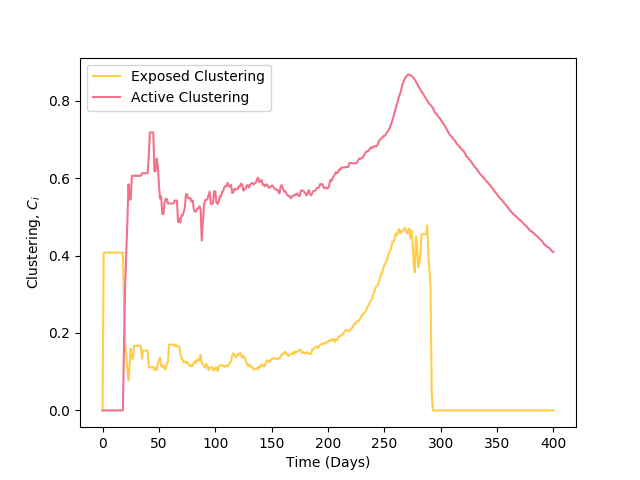
\includegraphics[width=0.9\linewidth]{rev-abm/clustering2.png}
		\caption{Clustering}
		\label{fig:clustering-rev-abm}
	\end{subfigure}%
\\
	\begin{subfigure}{\textwidth}
		\centering
		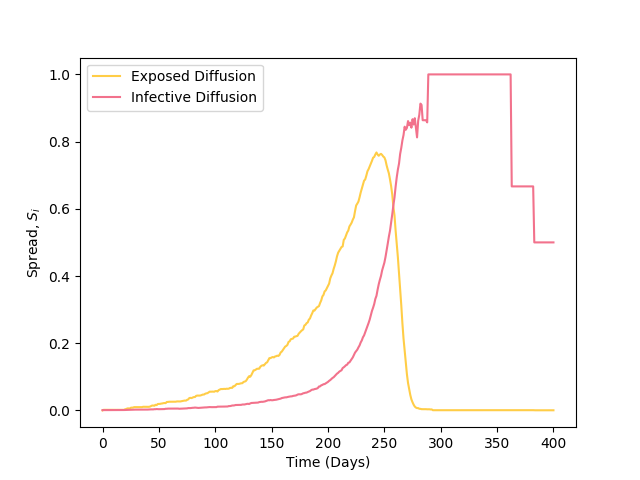
\includegraphics[width=0.9\linewidth]{rev-abm/diffusion2.png}
		\caption{}
		\label{fig:diffusion-rev-abm}
	\end{subfigure}
	\caption{Clustering and spread in the revolution ABM with default parameters. Figure \ref{fig:clustering-rev-abm} shows that the active population is consistently more clustered than the exposed population. Figure \ref{fig:diffusion-rev-abm} shows that the exposed class increase their spread through the population before being suddenly depleted near the peak of the revolution as they convert to the rapidly burgeoning active population.\label{mmd}}
	\label{fig:clustering-diffusion-rev-abm}
\end{figure}
\\
\begin{tcolorbox}
	\paragraph{Lesson for revolutionaries:} Ideas travel further than action. The idea can be widely distributed and lie dormant until action reaches it.
\end{tcolorbox}
\section{The Empire Strikes Back}
An interesting option is to introduce an adversarial agent to the model: the regime. It is an interesting question to ask what tactics they should adopt. In the previous model we have an equal chance of each active individual being removed. Instead we allow the option of the regime removing nodes based on their properties.\\
%\\
%To distinguish this from the current case, it would be most revealing to simulate on an Barab\'asi-Albert graph as this has a probability distribution closer to real world networks and will provide more insight into a principle that relies on the distribution of node degree.\\
\\
To stop the revolutionary idea spreading the regime wants to limit the number of nodes the idea can reach. The most effective way to do this is to separate the graph into two components with one containing all active revolutionaries and the other containing the rest. This means the regime could use Menger's Theorem to disconnect the graph efficiently.
%\textit{Mark: tell us what Menger's theorem is}
\label{mmd}
Menger's Theorem states that the minimum number of nodes one needs to remove to disconnect two disjoint subgraphs $U, V\subset V(G)$ is equal to $k$, the number of distinct paths from $U$ to $V$\cite{graph-theory-reference}. In our example $U$ can be the set of exposed and infective nodes and $V$ the set of susceptible and removed nodes. These are clearly disjoint as a node is in exactly one of these states at one time so Menger's theorem for these two sets. The regime could then instantaneously remove $k$ active nodes to disconnect the two subgraphs. 
However, the assumption that the regime is able to identify and efficiently take out just the nodes that will separate the graph is incredibly strong, requiring exact knowledge of the network and the ability to pick out any individual.\\
\\
Instead we assume that the regime becomes aware of revolutionaries only through attempted contacts with susceptibles. With this ability, what is the best option for the regime? It makes sense for them to pick out active revolutionaries with the highest number of contacts. This makes the problem one of attack tolerance in networks\cite{attack-tolerence-network}. In practice this means that more high-profile revolutionaries are at greater risk. This is based on the idea everyone is at some risk and this is proportional to the number of contacts $p\hat n$ they can and do make. Based on historical evidence this is often what happens: regimes target high-profile individuals both because they are more easily detected as well as them making a better example. Whilst this can provoke the populace it can also serve to provide a split in tactics and leadership. For these reasons we will consider this option.\\
\\
Some graphs are more resilient to this targeted node removal than others. Scale-free graphs have a low attack tolerance as removing just a few supernodes can drastically disconnect the graph. However, in a more egalitarian network such as the Watts-Strogatz network or Erd{\H{o}}s-R{\'{e}}nyi graph this is harder to do\cite{attack-tolerence-network}.\\
\\
Some naturally occurring networks seem to be naturally catered to tolerating attacks and failures. The social network of the bottlenose dolphins community of Doubtful Sound fjord has been studied in detail and shows an unusually high level of interconnection with no clear hubs and also low clustering\cite{dolphin-network}. The network was found by taking observations of a community of 64 dolphins over 6 years. There is an edge between two dolphins if they are seen together more often than expected by chance.
\label{mmd} The result of this network organisation is that if a few dolphins die it is very unlikely to break apart the social network and so they will stay as a single component. That is, they have evolved to have a high failure tolerance.\\
\\
The findings of the benefits of decentralised movements reflects a growing historical trend of egalitarian organisation in successful non-violent resistance\cite{battle-of-seattle}. As Eddie Yuen writes in \textit{The Battle of Seattle} on the trends that developed through the 20th century to lead to the increasing success of non-violent protest\cite{logic-non-violence} and in particular the Seattle protests against the WTO in 1999:
\begin{quote}
	The second [of these adoptions] is a commitment to direct democracy, as specifically the organisational forms of the affinity group, decentralized spokes-council meetings and consensus process.
\end{quote}
\begin{tcolorbox}
	\paragraph{Lesson for revolutionaries:} \textit{Be like a dolphin}. Decentralised and interwoven networks are more immune to targeted attacks. Pursue organisational structures which avoid unnecessary hierarchy by pursuing tactics such as direct democracy.
\end{tcolorbox}
%\section{Revolution on a Network}
%\subsection{Model Specification}
%This model involves one category of actors: 'citizens'. Following Epstein\cite{epstein}, we include two exogenous factors: hardship ($H$) and legitimacy ($L$).\\
%$H$ 
%\subsection{Agent Specification}
%They are members of the general population and may be in one of four states: susceptible ($S$), inactive revolutionaries ($I_1$), active revolutionaries ($I_2$), and removed ($R$). As in many agent-based models, they are heterogeneous in many respects.


\chapter{Explorations in games on networks}\label{ch:games-on-networks}
\section{Game theory}
\subsection{Prisoner's Dilemma}\label{subs:prisoners-dilemma}
The Prisoner's Dilemma is the canonical game of game theory finding its use in models for everything from how firms price goods\cite{p-d-goods} to sharing in vampire bats\cite{p-d-nature}. In any situation where there is the possibility of cooperation, the Prisoner's Dilemma can be a useful model in understanding the situation to a first approximation.\\
\\
%\paragraph{The Story}
The motivating story goes that two accomplices are caught at a crime scene, arrested and placed in separate cells with no contact. The police give them each a choice: they can confess their crimes to the authorities or they can stay silent. They learn that if they both stay silent, they only get one year in prison. If they both confess, they both get two years. However, if one of them confesses and the other stays silent, the snitch gets out immediately while the snitched-upon gets 3 years. As they are in separate cells, they cannot communicate.\\
\\
The smallest combined time in prison for the couple is if they both stay silent and take 1 year in jail each. But even if they could communicate and agree to the appealing option of both staying silent, it would still make sense to defect from the `contract' and confess. Just 1 year in jail is clearly better than 2. How should they work through this? As with most things in life, they should get mathematical.
\subsubsection{Making this mathematical}
%\paragraph{Key Concepts}
This story has all the features of a game-theoretic game. Let's go through it, pick out the key elements and name them.\\
\\
The four essential elements of a game have a useful acronym: \textit{PAPI}\cite{rasmusen_2010}. This stands for:
\begin{enumerate}[nosep]
\item \textbf{P}layers of the game,
\item \textbf{A}ctions available to each player,
\item \textbf{P}ayoffs for each outcome
\item \textbf{I}nformation available to each player.
\end{enumerate}
\par\null\par
In our story, there are two players: Lou and Avery. There are two actions available to them: stay silent or confess.  The payoffs are given by the years in jail, $-x$ for $x$ years in jail. As they cannot communicate, there is no information available about the other player's choice prior to choosing.\\
\\
Formally, we call staying silent a decision to \textit{cooperate} with the partner. We also say that to confess is to \textit{defect} from their partner. We usually notate actions as a single letter. Here we write $C$ for cooperate and $D$ for defect. An \textit{outcome} defines an action for each player. It can be written $(C,C)$ for two players both playing the action $C$.\\
\\
%\subsubsection{Representing games}
%\subsubsection{Payoff Matrix}
A payoff matrix is a way of defining two-player simultaneous games completely\cite{osborne}. This means that it tells you about every element of \textit{PAPI}. The payoff matrix for the Prisoner's Dilemma given in the story would be:\\
\setlength{\extrarowheight}{2pt}
\begin{tabular}{cc|c|c|}
	\centering
	& \multicolumn{1}{c}{} & \multicolumn{2}{c}{Avery}\\
	& \multicolumn{1}{c}{} & \multicolumn{1}{c}{$C$}  & \multicolumn{1}{c}{$D$} \\\cline{3-4}
	\multirow{2}*{Lou}  & $C$ & $(-1,-1)$ & $(-3,0)$ \\\cline{3-4}
	& $D$ & $(0,-3)$ & $(-2,-2)$ \\\cline{3-4}
\end{tabular}
\\
\\
\\
The ordered pair $(x,y)$ in each matrix entry gives the payoffs for each outcome. $x$ gives the payoff for the horizontal player and $y$ gives the vertical player's. So outcome $(D,C)$ has payoff $(0,-3)$ meaning a payoff of $0$ for Lou for defecting and a payoff of $-3$ for Avery for cooperating. The players, actions and payoffs are defined. Also, in a simultaneous game there is no information available about the other player's action. So this matrix does indeed completely describe the game.\\
\\
The payoff matrix is an extremely useful representation, allowing concise, complete descriptions of games. Consider, for example:\\
\setlength{\extrarowheight}{2pt}
\begin{tabular}{cc|c|c|c|}
	& \multicolumn{1}{c}{} & \multicolumn{3}{c}{Avery} \\
	& \multicolumn{1}{c}{} & \multicolumn{1}{c}{$R$}  & \multicolumn{1}{c}{$P$}  & \multicolumn{1}{c}{$S$} \\\cline{3-5}
	& $R$ & $(0,0)$ & $(-1,1)$ & $(1,-1)$ \\ \cline{3-5}
	Lou  & $P$ & $(1,-1)$ & $(0,0)$ & $(-1,1)$ \\\cline{3-5}
	& $S$ & $(-1,1)$ & $(1,-1)$ & $(0,0)$ \\\cline{3-5}
\end{tabular}
\\
\\
\\
This game might initially look foreign, but it is simply Rock, Paper, Scissors. You can create stories to motivate them but the payoff matrix completely defines all the relevant mathematical aspects of the game. This allows us to abstract from the messy details of the human world and find `solutions' to the game.
\subsubsection{Strategies and solution concepts}
A \textit{strategy} is a set of rules that determine which action a player will use at each point of the game. Note that as the Prisoner's Dilemma has only one point to make a decision, a strategy determines just one action. Further a strategy profile determines a strategy for each player in the game. There are various ways to discuss the effectiveness of strategies and strategy profiles in a game.\\
\\
%\subsubsection{Strategies}
%\paragraph{Socially Optimal Strategy}
The \textit{socially optimal strategy profile} is the strategy profile that leads to the highest joint payoff for all players. That is, the sum of the payoffs is the highest of all possibilities. In this game this is the easily identifiable and clearly optimal option of both players cooperating so that they get only 1 year each.\\
\\
%\paragraph{Nash Equilibrium}
However, the outcome with both defecting is the \textit{Nash Equilibrium}. Informally, the Nash Equilibrium is an outcome in which, even if all players knew almost telepathically what the other player's actions were going to be, none of them would choose to change their action as it would not improve their payoff. In this game, both players defecting, $(D,D)$, is the unique Nash Equilibrium. This is because if one player, say Lou, knew that Avery would play $D$ he would not change to $C$. Similarly for Avery.\\
\\
%\paragraph{Dominant Strategy}
The outcome of $(D, D)$ actually satisfies an even stronger condition as the action $D$ is a \textit{dominant strategy} for both players. This means that no matter what action the opponent plays, the player will always get the best payoff by defecting. This is how $(D,D)$ manages to `pull' players in, despite it having a worse payoff for both players than $(C,C)$.\\
\\
So we have described three solution concepts. Which one do we predict will happen? Game theory assumes that players are \textit{rational}. This means that the payoffs match the player's desires and they desire to increase their payoff. In other words the payoffs accurately describe their preferences. If Lou and Avery are rational, they will always end up both defecting, betraying each other and being rewarded with a longer jail term. So it goes.
\subsection{Repeated games}\label{subs:repeated-games}
%\subsubsection{Introduction}
The Prisoner's Dilemma is a \textit{one-shot game}. This means that no further games are played after the first game. It happens once and never again, with no possible repercussions that are not already described in the payoff matrix.\\
\\
Unlike one-shot games, repeated games have players play multiple games against each other. Whereas before a strategy determined just one action, in a repeated game a strategy can respond to the other player's actions. This means that it is harder or even impossible to `solve' these games to find the best actions and equilibria. However, this makes them more interesting, allowing for complex dynamics.
\subsubsection{Iterated Prisoner's Dilemma}
If we have two players playing the Prisoner's Dilemma repeatedly against each other we create the Iterated Prisoner's Dilemma. This no longer has a best strategy.\\
\\
In the absence of an analytically provable `best' strategy, we can pursue a more empirical approach. In football we cannot prove a-priori the best team. Indeed it would be a bit boring if we could. Instead, we create a tournament such as the Premier League and declare the winner of the tournament the `best' team. Inspired by this approach, we create a `tournament' of different strategies all playing several hundred games of the Prisoner's Dilemma against each other. The winner of the tournament will be the strategy with the highest payoff overall.\\
\\
This numerical experiment was famously first done by Robert Axelrod\cite{axelrod} in the 1980s. In Axelrod's first tournament, the winner was `Tit for Tat', a strategy that always cooperates on the first round and then copies the opponent's previous move forever after. Since then other researchers have repeated the tournament and Axelrod himself ran a second tournament with many more entries. A recent open-source collaboration makes it easy to replicate the Axelrod's original tournament as well as run similar ones\cite{axelrod-github}.\\
\\
For the tournament, we choose to enter five strategies: Tit for Tat, Defector, Cooperator, Alternator and Random. The names are descriptive: Defector always defects, Cooperator always cooperates, Alternator alternates between the two and Random chooses between the two actions with probability $0.5$ at each point. They play against every other strategy $10$ times. They also play against themselves $10$ times. The payoffs are also altered to fit Axelrod's first tournament. They are given by $1$ for two defectors, $3$ for two cooperators and $5$ and $0$ for the defector and cooperator respectively.\\
\setlength{\extrarowheight}{2pt}
\begin{tabular}{cc|c|c|}
	& \multicolumn{1}{c}{} & \multicolumn{2}{c}{Avery}\\
	& \multicolumn{1}{c}{} & \multicolumn{1}{c}{$C$}  & \multicolumn{1}{c}{$D$} \\\cline{3-4}
	\multirow{2}*{Lou}  & $C$ & $(3,3)$ & $(0,5)$ \\\cline{3-4}
	& $D$ & $(5,0)$ & $(1,1)$ \\\cline{3-4}
\end{tabular}
\label{mmd}
\\
\\
Running the tournament reveals that `Defector' does best in this tournament (Fig. \ref{fig:iterated-p-d-tournament}). The key point is that there is no single strategy that dominates all the others. Whilst `Defector' does best in this tournament, with a different selection of strategies it probably would not. Indeed it was entered into Axelrod's first tournament and was beaten by Tit for Tat, a strategy it won against here. Whilst this may seem paradoxical it is no more paradoxical than a polar bear being better suited to Antarctica than a tiger but would struggle in Bali. That is, the strategies success is dependent on its environment. In it's extreme, a defector does well in a tournament full of unquestioning cooperators. However, in a tournament full of Tit For Tat strategies, the Tit for Tat strategies get consistently high payoffs through cooperation which the defector misses out on, instead getting the spoils of mutual defection.\label{mmd}
%\textit{Mark: This seems paradoxical - what is it about the tournament design that makes this possible?}
\begin{figure}
	\centering
	\begin{subfigure}{\textwidth}
		\centering
		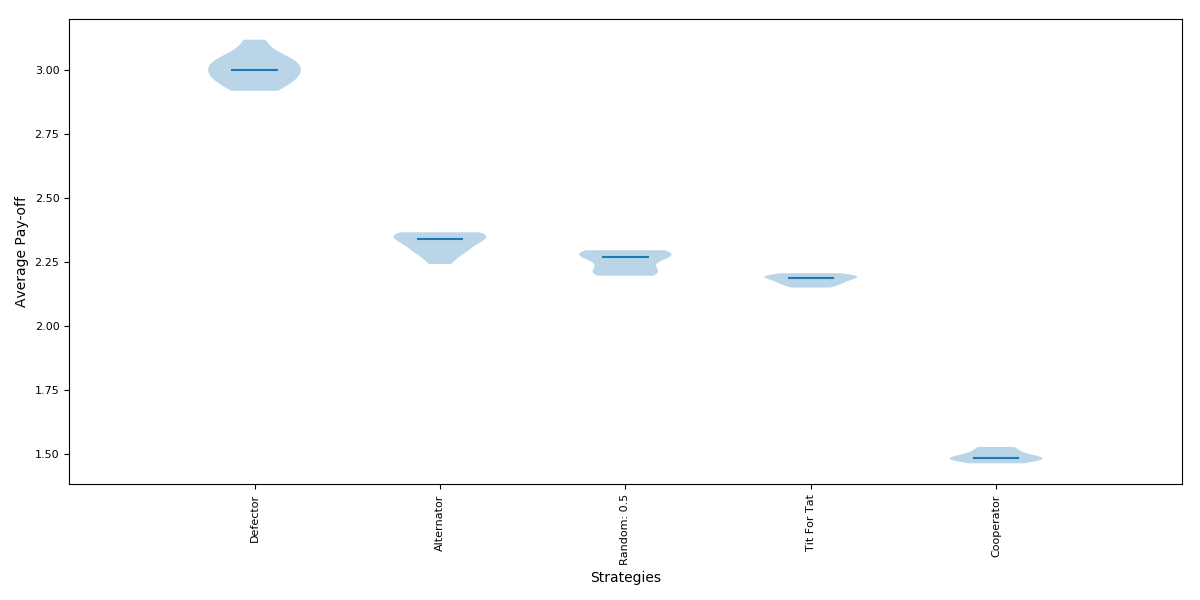
\includegraphics[width=\linewidth]{axelrod/tournament-boxplot.png}
		\caption{The results of a tournament of the Prisoner's Dilemma between 5 strategies. The tournament was repeated 100 times. Due to the strategy `Random' the results were different each time. The plot shows the average payoff between all tournaments in the solid blue line and the shaded blue region represents the variance.
%		\textit{Mark: I don't understand this figure}
		\label{mmd}
		}
		\label{}
	\end{subfigure}%
\\
	\begin{subfigure}{\textwidth}
		\centering
		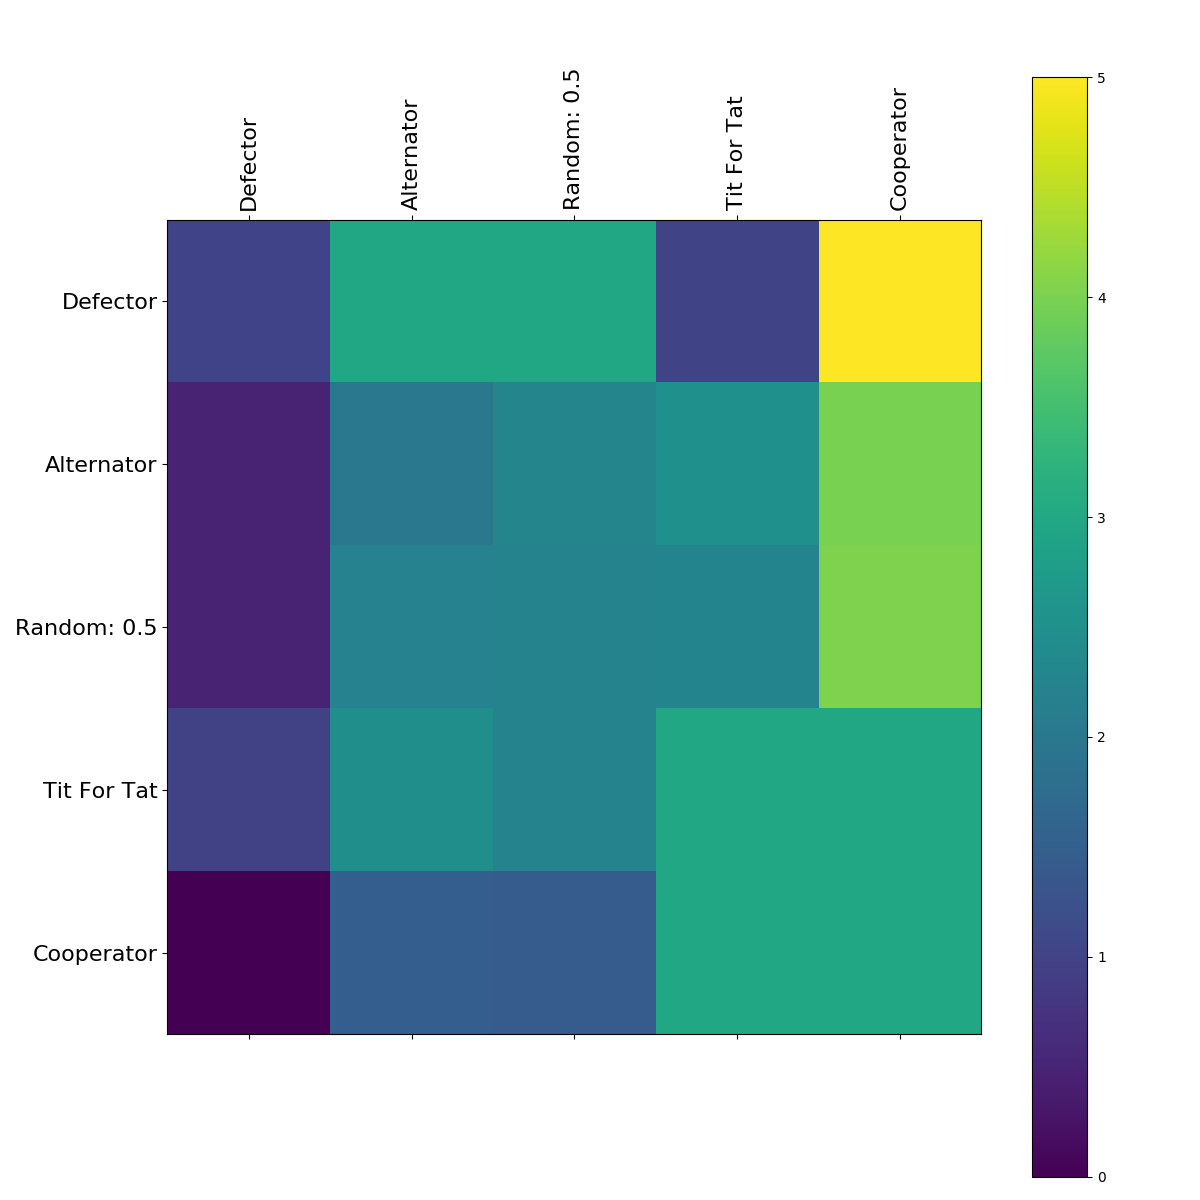
\includegraphics[width=0.95\linewidth]{axelrod/tournament-payoff-matrix.png}
		\caption{A payoff matrix showing how each strategy performed on average against the other strategies. The colour of the point $(X,Y)$ represents the score of strategy $X$ playing against strategy $Y$.}
		\label{}
	\end{subfigure}
	\caption{A tournament of the Iterated Prisoner's Dilemma between five strategies.}
	\label{fig:iterated-p-d-tournament}
\end{figure}\\
\\
We can create a grand competition with 222 different strategies. The strategies comprise every entry from a library of distinct strategies submitted to the Axelrod-Python project team\cite{axelrod-github}.\label{mmd} On this run the joint winners were: `Hard Prober', `Pun1' and `Tester'. For example Hard Prober's strategy is to play $D,D,C,C$ initially. This is to act as a test to see how cooperative its opponent is. If the opponent cooperated in moves 2 and 3, Hard Prober will defect forever. Otherwise, it will play Tit-For-Tat for the rest of time. The results of the tournament are messy to see as a plot, payoff matrix or indeed a table of the raw data. However, the alphabetically first 5 strategies are shown in Fig. \ref{fig:222}.
%\begin{tabular}{1|1}
%	\csvreader[head to column names]{images/csv/axelrod-tournament-222.csv}{}
%	{\\\hline\csvcoli&\csvcolii}
%\end{tabular}
\begin{figure}
\csvautotabular{../data/axelrod-tournament-222-short.csv}
\caption{A table of the alphabetically first 5 strategies in an iterated Prisoners Dilemma tournament of 222 different strategies.}
\label{fig:222}
\end{figure}
\subsubsection{Iterated games with evolution}
One natural extension to iterated games is to allow the possibility of `evolutionary' behaviour. For example, we can create simulations where strategies with higher payoffs are more likely to produce `offspring'. This means that the number of players using a successful strategy tends to increase.\\
\\
This can be imagined in the ordinary evolutionary sense of survival of the fittest. However, there is another useful interpretation. We can view the population as a constant group of players who are open to the possibility of changing their strategies. If they see a strategy that is working better, there is some probability that they use that strategy in the next iteration.\\
\\
We randomly select $7$ players using strategies from Axelrod's tournament. We play them off each other and themselves. After each round, they have some chance of `reproducing' proportional to the payoff they just received from playing every other player. Then the next round has a population that tends to have more of the successful strategies and less of the poorly adapted strategies. A graph describing this is given in Fig. \ref{fig:moran-100}.
\begin{figure}
	\centering
	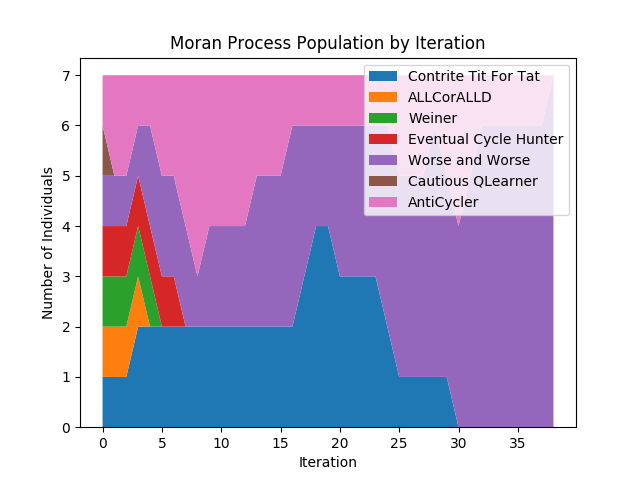
\includegraphics[width=\linewidth,trim={0 0 0 2cm},clip]{axelrod/iterated-moran-7.png}
	\caption{A graph showing an evolutionary prisoner's dilemma tournament.\label{mmd}. At each iteration or tick one agent is chosen to reproduce and one agent is chosen to die. The probability that they are chosen to reproduce is proportional to their payoff in the previous round.}
	\label{fig:moran-100}
\end{figure}
\\
\\
%[Include replicator equations at some point here.]\\
%For example, we can also try it with different gamesbelow is a simulation of strategies playing Rock, Paper Scissors defined by the payoff matrix as above.\\
%(
%My simulation of Rock, Paper, Scissors
%)\\
%The effect is a self-balancing system. If the strategy \textit{rock} becomes more populous, \textit{paper} will start to get higher payoffs on average. This in turn brings the population back towards $\frac{1}{3}$ for each strategy.\\
%The same scenario works with the admittedly less well-known game Rock, Paper, Scissors, Spock\cite{for game}\cite{for code}.\\
%(
%My simulation of Rock, Paper Scissors, Spock
%)\\
%However, now with the different rules we can have the extinction of strategies.
We can explore the same evolutionary set-up but with the game of Rock, Paper, Scissors. Whereas evolutionary Prisoner's Dilemma resulted in one strategy eventually monopolising the population, the evolution of Rock, Paper, Scissors results in a self-balancing system (Fig. \ref{rock-paper-scissors-evo}). For example if the strategy Rock becomes more populous, Paper will start to get higher payoffs on average. This gives Paper a higher chance of reproducing resulting in Paper reproducing at a quicker rate. This holds for all three pairs. So the population has an inbuilt tendency to return the population demographic back towards $\frac{1}{3}$ for each strategy.\label{mmd}
\begin{figure}
	\centering
	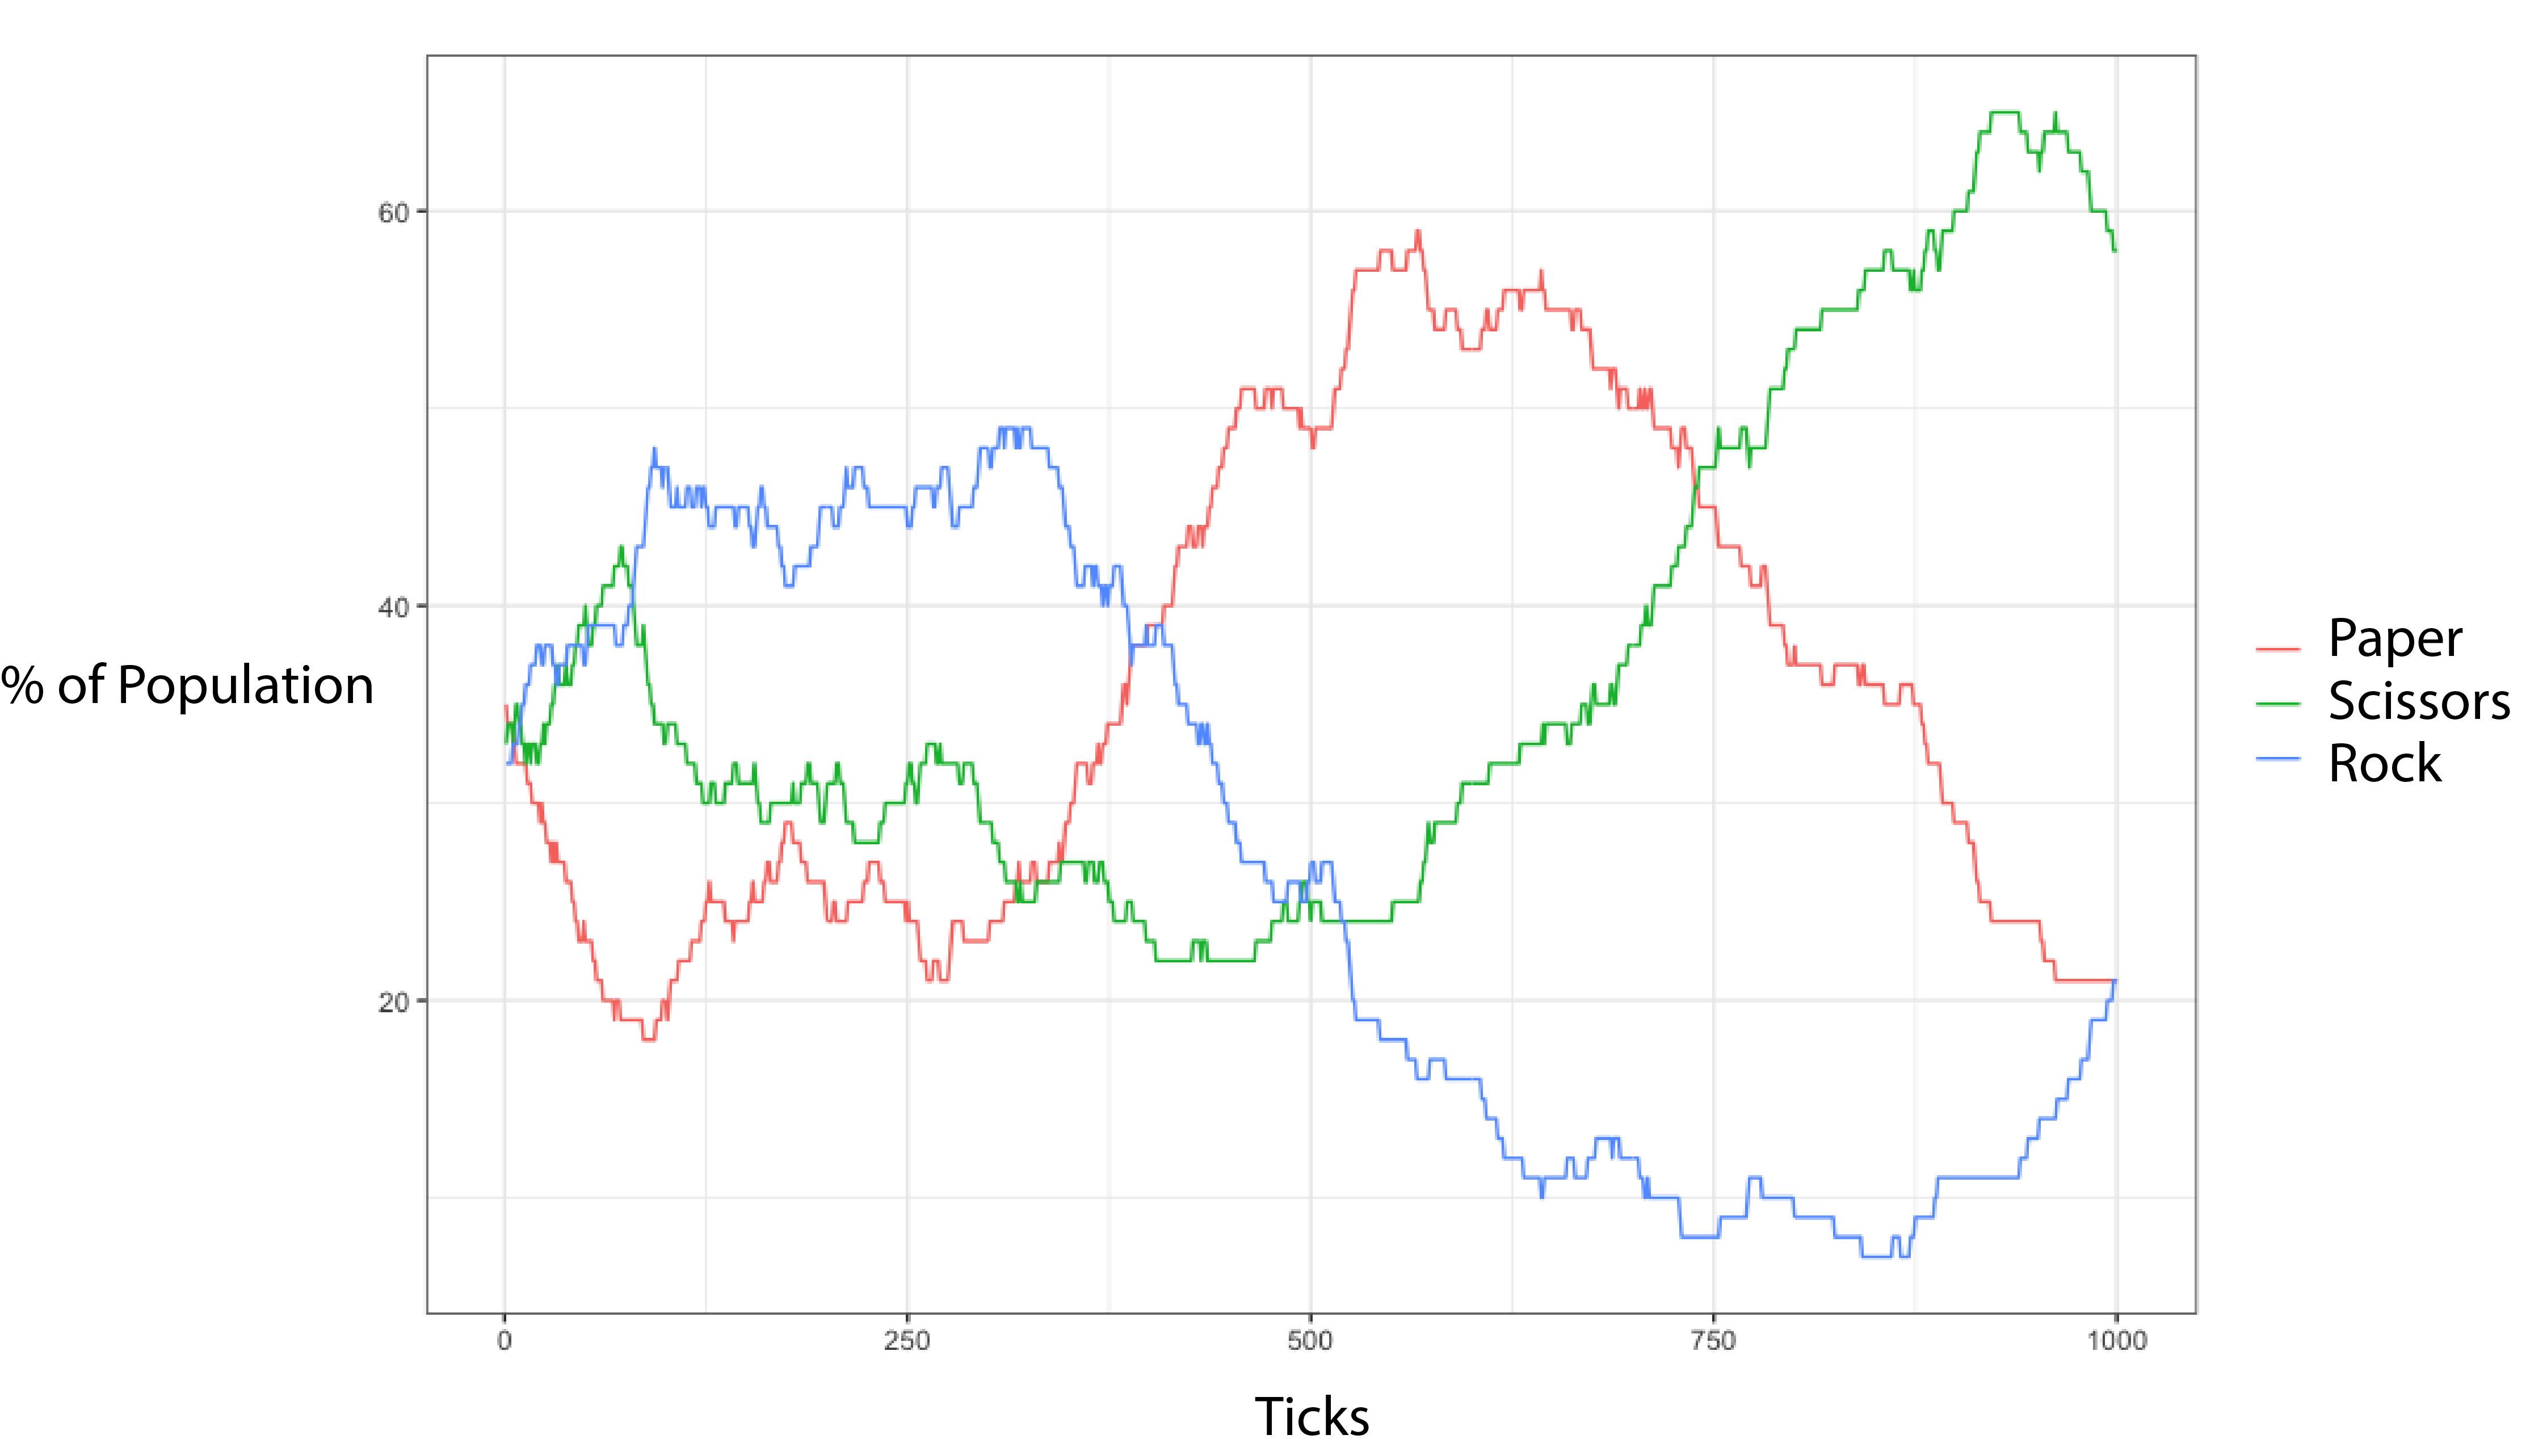
\includegraphics[width=\linewidth]{axelrod/rock-paper-scissors.png}
	\caption{An evolutionary game of Rock, Paper, Scissors. The graph shows the percentage of players changing through time.}
	\label{rock-paper-scissors-evo}
\end{figure}
\section{Graph theory}\label{sec:graph-theory}
%motivation
The tools we have built so far are helping us move closer to a reasonable description of real, complex situations. In real life, games are not usually isolated situations that happen as if in a laboratory. They happen around lots of other players and allow the possibility of a change of strategy. They are also interdependent with games in some places effecting others. If a person was playing the Prisoner's Dilemma and played against several defectors consecutively, they are more likely to defect themselves. We have begun to model this.\\
\\
However, players are in general not connected to every other player. They exist in communities. To model this we need graphs.\\
\\
\subsection{Definitions}
A \textit{graph} $G=(V,E)$ is a set of vertices $V$ and a set of pairs of vertices $E$. Each pair of vertices is called an edge. For now we will consider only undirected graphs with no loops . \textit{Undirected} means that the edge $(u,v)$ is identical to the edge $(v,u)$. That is to say, the pairs constituting the edges are unordered\cite{graph-theory-reference}. The requirement of no loops means that no vertex has an edge from itself to itself. Formally, $\nexists v\textnormal{ such that } (v,v)\in E$. We can see visually what this means in Fig. \ref{fig:example-graphs}.
\begin{figure}
	\centering
	\begin{subfigure}{.3\textwidth}
		\centering
		\includegraphics[width=.9\linewidth]{appendix/graph-theory/directedGraph.png}
		\caption{Directed graph}
		\label{fig:dir}
	\end{subfigure}%
	\begin{subfigure}{.3\textwidth}
		\centering
		\includegraphics[width=.9\linewidth]{appendix/graph-theory/loopGraph.png}
		\caption{Graph with loops}
		\label{fig:loop}
	\end{subfigure}
	\begin{subfigure}{.3\textwidth}
		\centering
		\includegraphics[width=.9\linewidth]{appendix/graph-theory/graph.png}
		\caption{Undirected graph without loops}
		\label{fig:undirected}
	\end{subfigure}
	\caption{We will consider graphs of type \ref{fig:undirected} and ignore the others.}
	\label{fig:example-graphs}
\end{figure}
\\
\\
Two vertices $u,v$ are \textit{adjacent} if and only if $(u,v)\in E$. The neighbourhood of a vertex $v$ in a graph $G$ is the induced graph given by $v$ and all vertices adjacent to $v$. That is, it is the graph of vertex $v$ and all vertices adjacent to $v$ with edges given by the edges between any of these vertices in $G$. As such we also call the adjacent vertices \textit{neighbours}.\\
\\
%Some common graphs
A useful graph that comes up repeatedly is the \textit{complete graph, $K_n$}. This is the graph with $n$ vertices with an edge between all pairs of vertices. Formally $K_n=\{\{v_1,...,v_n\},\{(v_i,v_j):\forall i\neq j\}\}$.
\begin{figure}
	\centering
	\begin{subfigure}{.5\textwidth}
		\centering
		\includegraphics[width=.9\linewidth]{appendix/games-on-networks/K5.pdf}
		\caption{$K_5$}
		\label{fig:K5}
	\end{subfigure}%
	\begin{subfigure}{.5\textwidth}
		\centering
		\includegraphics[width=.9\linewidth]{appendix/games-on-networks/K16.pdf}
		\caption{$K_{16}$}
		\label{fig:K16}
	\end{subfigure}
	\caption{The Complete Graphs $K_5$ and $K_{16}$}
	\label{fig:complete-graphs}
\end{figure}
\subsection{Graphs and the 2D lattice}
A graph often used in models is an adaptation of the 2D lattice as it is both instructive, relatively easy to analyse and most importantly easy to visualise\cite{eq_of_life}. The 2D lattice can be made by imagining a square grid, rows and columns of squares.
%\begin{figure}
%	\centering
%	\includegraphics[width=.5\linewidth]{appendix/graph-theory/square-grid.png}
%	\caption{A square grid}
%\end{figure}
However, we want to convert this into a graph. We can deal with the vertices easily: we put a vertex at the centre of each square. However there are multiple ways to define the edges. Which squares should be considered neighbours of each other?\\
\\
One option is to define the von Neumann neighbourhood of the 2D lattice as in Fig. \ref{fig:vonneumann}. This makes each point a neighbour of the $4$ points vertically and horizontally next to it. An alternative is given by the Moore neighbourhood as seen in Fig. \ref{fig:moore}. This includes the nearest vertical and horizontal neighbours as well as the nearest diagonal points\cite{eq_of_life}.
\begin{figure}
	\centering
	\begin{subfigure}{.5\textwidth}
		\centering
		\includegraphics[width=.9\linewidth]{appendix/graph-theory/von-neumann-neighbourhood.png}
		\caption{The von Neumann Neighbourhood}
		\label{fig:vonneumann}
	\end{subfigure}%
	\begin{subfigure}{.5\textwidth}
		\centering
		\includegraphics[width=.9\linewidth]{appendix/graph-theory/moore-neighbourhood.png}
		\caption{The Moore neighbourhood}
		\label{fig:moore}
	\end{subfigure}
	\caption{Different definitions of `neighbourhood' on the 2D Lattice}
	\label{fig: lattice neighbourhoods}
\end{figure}\\
\\
The graphs given by these two definitions are given in Fig. \ref{fig:graph-neighbourhoods}. The graph induced by the von Neumann neighbourhood is often called the grid graph, lattice graph. The graph induced by the Moore neighbourhood is also called the King's Graph as it represents the legal moves of a king in a game of chess.
\begin{figure}
	\centering
	\begin{subfigure}{.47\textwidth}
		\centering
		\includegraphics[width=\linewidth]{appendix/graph-theory/grid-graph.png}
		\caption{}
		\label{fig:graph-v-n}
	\end{subfigure}
	\begin{subfigure}{.47\textwidth}
		\centering
		\includegraphics[width=\linewidth]{appendix/graph-theory/kings-graph.png}
		\caption{}
		\label{fig:graph-m}
	\end{subfigure}
	\caption{Graph representation of the 2D lattice with the von Neumann neighbourhood\ref{fig:graph-v-n} and the Moore neighbourhood \ref{fig:graph-m}}
	\label{fig:graph-neighbourhoods}
\end{figure}\\
\\
Typically to avoid boundary effects when playing games on these lattices we `wrap' the 2D lattice. This creates a torus. So each vertex displayed visually at the top of the lattice is joined to the neighbour in the same column at the bottom of the lattice. This avoids, for example, the side players having fewer opponents. However it makes it harder to visualise explicitly and so is normally drawn in two-dimensions with no visual representation of the wrapping.
\section{Games on networks}
%\subsubsection{Games on graphs we have already seen}
Having further built up our tool-kit, we can now consider games on graphs. We set each vertex to represent a player and only allow players to play a game against players they are adjacent to. In fact, we have sneakily been doing this the whole time but now we want to make this explicit.\\
\\
The basic Prisoner's Dilemma in \ref{subs:prisoners-dilemma} was a game on a trivial graph $G=(\{Lou,Avery\},\{(Lou,Avery)\})$, visualised in Fig. \ref{fig:p-d-graph}.
\begin{figure}[h]
	\centering
	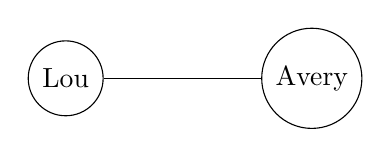
\begin{tikzpicture}
	\draw
	(1,1) node[anchor=east,circle,draw]{Lou}--
	(3,1) node[anchor=west,circle,draw]{Avery};
	\end{tikzpicture}
	\caption{The trivial graph underlying the one-shot Prisoner's Dilemma}
	\label{fig:p-d-graph}
\end{figure}
Similarly, for the Iterated Prisoner's dilemma tournament if we call the players $p_1,...,p_n$, the tournament was a repeated game on a complete graph $K_n$.\\
\\
%\subsubsection{Some new Graphs}
So we were already playing games on graphs implicitly. Now we can try building games while noting the graphs we are playing on explicitly and seeing what effect this has.
\subsection{Prisoner's Dilemma on a torus}\label{p-d-torus}
%\subsubsection{Set-up}
We can extend the Iterated Prisoner's Dilemma to a tournament on a 2D lattice. Firstly, we make an $n \times n$ grid with wrapped ends to avoid boundary effects, creating a torus. Using the process seen in the previous section we make a graph out of this using the Moore neighbourhood. Then we let each vertex be a player of the Prisoner's Dilemma. They play against all other vertices in their neighbourhood\cite{eq_of_life}.\\
\\
To initialise the system, in the first round each player plays $C$ with probability $p$ and $D$ with probability $(1-p)$. They play this action simultaneously against every neighbour, using the same strategy against each of them.\\
\\
For every round after, each player looks at their neighbour's scores from the previous round. They adopt the action of the highest scoring neighbour as their action for the next round\footnote{For most parameter values chosen, ties are only possible between cells that use the same strategies and so this is well-defined. If there were to be a tie between two distinct strategies, the strategy adopted would arbitrarily be the strategy closest to the top left of the grid.}\label{mmd} They then play this action against every neighbour.\\
\\
The payoff matrix retains characteristics of the matrix originally given for the Prisoner's Dilemma and is given by:\\
\setlength{\extrarowheight}{2pt}
\begin{tabular}{cc|c|c|}
	& \multicolumn{1}{c}{} & \multicolumn{2}{c}{Avery}\\
	& \multicolumn{1}{c}{} & \multicolumn{1}{c}{$C$}  & \multicolumn{1}{c}{$D$} \\\cline{3-4}
	\multirow{2}*{Lou}  & $C$ & $(1,1)$ & $(\epsilon,b)$ \\\cline{3-4}
	& $D$ & $(b,\epsilon)$ & $(0,0)$ \\\cline{3-4}
\end{tabular}
\\
\\
where $\epsilon<1<b$.\\
\\
%\subsubsection{Example Runs}
To run this we simulate on a $100\times100$ grid and choose values $p=0.5$ and $\epsilon=0$. We can create a wide variety of dynamic behaviour, including chaos and bifurcations by adjusting the value of $b$. Note that $b$ is the payoff from defecting against a cooperative partner. Intuitively, it is the reward to true villains who defect against players who were hoping to cooperate.
\subsubsection{Qualitative analysis: equilibrium and chaos}
For $b>1.\bar{6}$, the board eventually tends to an equilibrium with mostly defectors (Fig. \ref{fig:p-d-torus-1.7}). Clearly the rewards of non-cooperation are too high to a sustain a more socially beneficial situation.
\begin{figure}
	\centering
	\begin{subfigure}{.3\textwidth}
		\centering
		\includegraphics[width=.9\linewidth]{appendix/games-on-networks/pd-torus/1b=17.png}
		\caption{Early}
		\label{}
	\end{subfigure}%
%	\begin{subfigure}{.3\textwidth}
%		\centering
%		\includegraphics[width=.9\linewidth]{appendix/games-on-networks/pd-torus/2b=17.png}
%		\caption{Developing}
%		\label{}
%	\end{subfigure}
	\begin{subfigure}{.3\textwidth}
		\centering
		\includegraphics[width=.9\linewidth]{/appendix/games-on-networks/pd-torus/3b=17.png}
		\caption{Equilibrium}
		\label{}
	\end{subfigure}
	\caption{The simulation running with $b=1.7$}
	\label{fig:p-d-torus-1.7}
\end{figure}
Conversely, for $b<1.6$, the simulation tends towards a static equilibrium of mainly cooperators (Fig. \ref{fig:p-d-torus-1.5}).
\begin{figure}
	\centering
	\begin{subfigure}{.3\textwidth}
		\centering
		\includegraphics[width=.9\linewidth]{appendix/games-on-networks/pd-torus/1b=15.png}
		\caption{Early}
		\label{fig:dir}
	\end{subfigure}%
	\begin{subfigure}{.3\textwidth}
		\centering
		\includegraphics[width=.9\linewidth]{appendix/games-on-networks/pd-torus/2b=15.png}
		\caption{Developing}
		\label{fig:loop}
	\end{subfigure}
	\begin{subfigure}{.3\textwidth}
		\centering
		\includegraphics[width=.9\linewidth]{appendix/games-on-networks/pd-torus/3b=15.png}
		\caption{Equilibrium}
		\label{fig:undirected}
	\end{subfigure}
	\caption{The simulation running with $b=1.5$}
	\label{fig:p-d-torus-1.5}
\end{figure}
Between these two parameter regions, exists the third which exhibits the most interesting behaviour with chaotic dynamics between cooperation and defection (Fig. \ref{fig:p-d-torus-1.63}).
\begin{figure}
	\centering
	\begin{subfigure}{.3\textwidth}
		\centering
		\includegraphics[width=.9\linewidth]{appendix/games-on-networks/pd-torus/1b=163.png}
		\caption{Early}
		\label{fig:dir}
	\end{subfigure}%
	\begin{subfigure}{.3\textwidth}
		\centering
		\includegraphics[width=.9\linewidth]{appendix/games-on-networks/pd-torus/2b=163.png}
		\caption{Developing}
		\label{fig:loop}
	\end{subfigure}
	\begin{subfigure}{.3\textwidth}
		\centering
		\includegraphics[width=.9\linewidth]{appendix/games-on-networks/pd-torus/3b=163.png}
		\caption{Dynamic equilibrium}
		\label{fig:undirected}
	\end{subfigure}
	\caption{The simulation running with $b=1.63$}
	\label{fig:p-d-torus-1.63}
\end{figure}
\subsubsection{Quantitative analysis: invasion}
The usual approach for understanding evolutionary games is to find the conditions under which one type can `invade' a population. An invasion is when a small group of one type can grow in a population of other types. To do this with our game we must analyse the situation from the level of individual squares.\\
\\
Firstly, we need to find the minimal area that we can isolate to study. A single cell plays against it's surrounding neighbours and so we must consider at least the $3\times3$ grid surrounding a cell. However, the cell then adopts the strategy of all of its best performing neighbours. So it must look at its neighbour's payoffs. But it's neighbours payoffs depend on the games \textit{they} have just played against \textit{their} neighbours. So, to know what strategy our single cell will adopt we have to consider the surrounding $5\times5$ grid\cite{eq_of_life}.\\
\\
We will call the small population of potential invaders the \textit{cluster} and the rest of the population the \textit{sea}. Then we call the cells that are in the sea touching the cluster the \textit{boundary}. The general strategy we have will be to look at the boundary separating the small cluster of invaders from the rest of the population. If the boundary cells have a neighbour in the cluster with a better tactic than their neighbours in the sea, they will change and the cluster will grow.\\
\\
Let's first consider the conditions under which defectors can invade cooperators. Imagine a single defector in a sea of cooperators (Fig. (\ref{fig:1-d-i})). After the first game, the defector gets a payoff of $8b$, the boundary cells all get $7$ while all members of the sea get $8$. So the boundary members look to see if $8b>8$. As the game specifies that $b>1$, this is always true and so regardless of the value of $b$ it grows to a $3\times3$ grid.
\begin{figure}
	\centering
	\begin{subfigure}{.49\textwidth}
		\centering
		\includegraphics[width=.9\linewidth]{appendix/games-on-networks/pd-torus/1-defector-invasion.png}
		\caption{1 defector invasion}
		\label{fig:1-d-i}
	\end{subfigure}%
	\begin{subfigure}{.49\textwidth}
		\centering
		\includegraphics[width=.9\linewidth]{appendix/games-on-networks/pd-torus/9-defector-invasion.png}
		\caption{9 defector invasion}
		\label{fig:9-d-i}
	\end{subfigure}
	\caption{Defector invasion}
	\label{}
\end{figure}\\
\\
So now we consider a $3\times3$ grid of defectors (Fig. (\ref{fig:9-d-i})). The sea cells always have a higher payoff ($8$) than the boundary (either $5,6$ or $7$). The highest scoring cell in the cluster is the edge cell with a payoff of $5b$. Every cell of the boundary is a neighbour to an edge cell. Hence each cell looks to see if $5b>8$. If it is, they change and the cluster grows. Otherwise, it stays the same or shrinks. So to have the possibility of defector invasion we need $b>8/5=1.\dot6$.\\
\\
Now we consider cooperator invasion. We firstly note that a single cooperator cannot invade a population due to the constraints on the payoff matrix (Fig. (\ref{fig:1-c-i})). The defectors can simply feed off the foolishness of the sole cooperator and it will die off. Hence a cooperator invasion must start with some cluster.
\begin{figure}
	\centering
	\begin{subfigure}{.3\textwidth}
		\centering
		\includegraphics[width=.9\linewidth]{appendix/games-on-networks/pd-torus/1-cooperator-invasion.png}
		\caption{1 cooperator invasion}
		\label{fig:1-c-i}
	\end{subfigure}%
	\begin{subfigure}{.3\textwidth}
		\centering
		\includegraphics[width=.9\linewidth]{appendix/games-on-networks/pd-torus/4-cooperator-invasion.png}
		\caption{4 cooperator invasion}
		\label{fig:4-c-i}
	\end{subfigure}
	\begin{subfigure}{.3\textwidth}
		\centering
		\includegraphics[width=.9\linewidth]{appendix/games-on-networks/pd-torus/9-cooperator-invasion.png}
		\caption{9 cooperator invasion}
		\label{fig:9-c-i}
	\end{subfigure}
	\caption{Cooperator invasions}
	\label{}
\end{figure}
\\
\\
Looking at a $2\times2$ cluster of cooperators (Fig. (\ref{fig:4-c-i})), it is easy to see that if $b>3/2$ the cluster will grow uniformly. Otherwise it will be immediately destroyed.\\
\\
With a $3\times3$ cluster of cooperators there are different possibilities for growth (Fig. (\ref{fig:9-c-i})). Cell $A$ looks at the payoff of cell $B$ which is $2b$ against the payoff of it's only cluster neighbour which has a payoff of $3$. So if $3>2b$ it will change. If this is the case $B$ and $C$ will also both change.\\
\\
However, if $b>3/2$ there is still the possibility of $B$ and $C$ changing whilst $A$ stays the same. The highest scoring neighbour of cells $B,C$ will be either $C$ with payoff $3b$ or the cluster cell with payoff $5$. So they look to see if $5>3b$. If so they will change and the cluster will grow. This will create a cross structure.
\begin{figure}[h]
	\centering
	\caption{The payoffs of cells around a $3\times3$ cluster of cooperators in a sea of defectors.}
	\label{fig:p-d-graph}
\end{figure}
To summarise defector clusters can grow if $b>8/5=1.6$ and cooperator clusters can grow if $1.\dot6=5/3>b$. So there are three distinct parameter regions
\begin{enumerate}
	\item $b<1.6$ Only cooperator clusters can grow
	\item $1.6<b<1.\dot6$ Both cooperator and defector clusters can grow\label{chaos}
	\item $1.\dot 6<b$ Only defector clusters can grow
\end{enumerate}
This analytical approach justifies the conclusions we drew qualitatively earlier. In particular, region \ref{chaos}., where both defectors and cooperators can grow, represents the chaotic region.
%\subsubsection{Prisoner's Dilemma on a Scale Free Graph}
%\subsubsection{On Different Networks}
%We can adapt this to a hexagonal lattice.
%\begin{figure}
%	\centering
%	\begin{subfigure}{.3\textwidth}
%		\centering
%		\includegraphics[width=.9\linewidth]{appendix/games-on-networks/pd-hexagon/0005.png}
%		\caption{}
%		\label{fig:dir}
%	\end{subfigure}%
%	\begin{subfigure}{.3\textwidth}
%		\centering
%		\includegraphics[width=.9\linewidth]{appendix/games-on-networks/pd-hexagon/0012.png}
%		\caption{}
%		\label{fig:loop}
%	\end{subfigure}
%	\caption{Running the evolutionary Prisoner's Dilemma on a hexagonal lattice}
%	\label{fig:p-d-torus-1.63}
%\end{figure}

\chapter{Conclusion}\label{ch:conclusion}
\section{Lessons from this paper}
Through this paper we have explored how mathematics can be used to model complex social systems from the evolution of cooperation to economic inequality. In particular we have focused on how to represent notions of agency and interrelations to develop two models of revolution inspired by mathematical epidemiology. The first compartmental model was able to provide many insights into the phenomena. However its clear restrictions showed the necessity of a more complex model. This led to the development of an ABM that could account for network dynamics and the inherent stochasticity of real life.

\section{Further work}
\subsection{Interesting theoretical extensions}
%This provides a suggestion for the general direction of research in this area. However there are also many smaller, lower-hanging fruit that would provide stimulating papers.
There are many possible routes for expanding this model. One possibility would be to more thoroughly investigate the role of supernodes in catalysing revolutions. For example Mohamed Bouazizi's highly symbolic self-immolation sparked the Tunisian revolution. More generally, people such as journalists and politicians have a unique reach and ability to spread a message. Modelling this would involve more careful study of how properties of scale-free graphs affect the revolution model as well as considering a probability distribution over the agents' $\beta$ values.\\
\\
Another option is to introduce the need for multiple contacts to be made before people truly take an idea on. This is based on the observation that social influence works quite differently to how diseases spread. In a paper on social contagion Thomas House justifies this approach\cite{thomas-house}:
\begin{quote}
[Experimental studies show] there is significant evidence that the form of ‘infection’ in social influence is different to that in a biological epidemic. The important difference is the number of exposures to infection that an individual must receive before becoming infected: in biological infection only one source of infection is required for a non-zero probability of infection, whereas in social influence multiple sources are required.
\end{quote}
Dodds and Watts have already built a model adopting the SIS model to this form of infection\cite{dodds-watts}. Future compartmental models of revolution should seek to accommodate a similar approach. It would also be both interesting and simple to adopt this idea into future ABMs too.\\
\\
A more data science flavoured extension would involve attempts to find more finely grained time series data on a revolution than currently available datasets\cite{NAVCO-2.0}. One interesting option would be to analyse sentiment data on Twitter during a revolution such as the Arab Spring. Whilst this is potentially very messy data it could be revealing. There is also some debate about the extent to which the Arab Spring was a `social media revolution'\cite{egypt-five-years}. A quantitative analysis of Twitter data throughout the Arab Spring would shed a light on this question.
%\\
%\\
%Specifically to ABMs, it would be revealing to perform this on a much larger network to more accurately model a population. To do so the algorithm would have to be improved. One way to do so would be to adopt a Hastings style algorithm.

\subsection{A suggestion for the general direction for the mathematical study of revolution}
The rigorous approach of Chenoweth's \textit{Why Civil Resistance Works: The Strategic Logic of Nonviolent Conflict}\cite{logic-non-violence} provides an important contribution to the quantitative analysis of revolutions. This text and accompanying dataset give a firm understanding of what the majority of successful revolutions in the last century have looked like: non-violent, democratic and broad-based. However, the text mainly offers a \textit{how}. The next step is to offer a \textit{why}.\\
\\
The goal of quantitative revolutionary research right now should be to account for these statistical findings. I believe a strong approach to explain their results theoretically is to pursue an epidemiologically-inspired route. The obvious next step in this direction would be to create a more nuanced ABM which is `tuned' to the data provided in the NAVCO dataset\cite{NAVCO-2.0}. This would involve including parameters such as the regime's legitimacy and the support of foreign states for the revolutionary campaign as inputs. In this way a desirable model would fuse the epidemiologically inspired models introduced in this paper with the global parameters present in Epstein's civil violence model\cite{epstein} and the hard data of the NAVCO dataset.

\chapter{Appendix}\label{ch:mathematical-background}
\section{Stability theory}\label{dynamical-systems}
A dynamical system is a system that evolves in time. Stability theory is concerned with finding and classifying equilibriums. These are states of the system that do not change with time. Many dynamical systems can be represented through differential equations. If the system of differential equations has $n$ variables, choosing any set of values for the variables defines a point $x\in\mathbb{R}^n$. As the differential equations describe some change in time, moving time forwards sees this point moves through the space $\mathbb{R}^n$. The path made by including all points passed through in a period of time is called a \textit{trajectory}.\\
\\
A \textit{fixed point}, $\bf{x}$, is a point at which, if there is no perturbation, the system will stay forever. It is a time-independent solution to the system. However, there are many different types of fixed point. The two basic classes are stable and unstable fixed points. Informally, a fixed point $x$ is stable if a small perturbation from the point will bring it back to $x$. Similarly, a fixed point is unstable if a small perturbation from the point $x$ makes the system move away from $x$.\\
\\
%Let's get a bit more specific with this. Three key concepts are attraction, liapanov stability and asymptotic stability.
Let $\bf{x}\in\mathbb{R}^n$ and $\bf{f}:\mathbb{R}^n\rightarrow\mathbb{R}^n$ such that $\bf{\dot x}=\bf{f}(\bf{x})$. This is a compact form of
\begin{equation}\label{eq:compact-form}
\frac{d}{dt}
\begin{bmatrix}
 x_1 \\
\vdots\\
x_n
\end{bmatrix}
=
\begin{bmatrix}
f_1(x_1,...,x_n) \\
\vdots\\
f_n(x_1,...,x_n)
\end{bmatrix}
\end{equation}
We say that $\bf{x}^*$ is a \textit{fixed point} of a dynamical system if $\bf{f}(\bf{x}^*)=\bf(0)$. Geometrically this means that this point would not move. $\bf{x}^*$ is also called an equilibrium.\\
\\
%Let $\bf{x}^*$ be a fixed point. We say that a point is \textit{attracting} if all trajectories starting near $x^*$ approach $x^*$ as time goes to infinity. Formally this means that 
%\begin{equation*}
%\lim_{t\rightarrow\infty}\norm{\bf{x}(t)-\bf{x}^*(t)} = 0
%\end{equation*}
%A point is \textit{stable} (or Liapanov stable) if all trajectories that start close to $x^*$ stay close to it for all time. Formally this means
%\begin{equation*} \forall\epsilon>0,\exists\delta>0\text{ s.t. }\norm{x(0)-x^*}<\delta\implies\norm{x(t)-x^*}<\epsilon,\forall t>0
%\end{equation*}
%A fixed point that is not (Liapanov) stable is \textit{unstable}\cite{Braun:1993kx}.\\
%\\
%More strongly, a fixed point is \textit{asymptotically stable} if it is both attracting and Liapanov stable. The difference between Liapanov and asymptotic stability is that a small perturbation from a (Liapanov) stable point will stay close. However, a small perturbation from an asymptotically stable point will return to the fixed point. Thus a pendulum without friction is Liapanov stable but a pendulum with friction is also asymptotically stable.
%https://www.cds.caltech.edu/~murray/courses/cds101/fa02/faq/02-10-23_lyapexact.html
We say $\bf{x}(t)$ is \textit{stable} if it is a solution of Eq. (\ref{eq:compact-form}) with initial condition $\bf{x}(t=0)=\bf{x_0}$ and $\forall \epsilon>0,\exists \delta>0$ such that if $\bf{x'}(t)$ is another solution of Eq. (\ref{eq:compact-form}) with $\bf{x'}(t=0)=\bf{x_0}'$ and $\norm{\bf{x_0'}-\bf{x_0}}<\delta$ then $\norm{\bf{x'}(t)-\bf{x}(t)}<\epsilon$ for all $t\geq0$\cite{Braun:1993kx}. Finally, a solution of Eq. (\ref{eq:compact-form}) that is not stable is \textit{unstable}\cite{Braun:1993kx}.
\subsubsection{Jacobian}
The stability of a point $\mathbf{x}$ can be investigated by considering the Jacobian matrix at that point. The Jacobian is the generalisation of a derivative, providing the best linear approximation of a function at a differentiable point.\\
\\
%Suppose we have a triple integral in the set of variables $x, y, z$:
%\begin{equation*}
%\int\int\int f(x,y,z)\,dx\,dy\,dz
%\end{equation*}
%Let $r, s, t$ be another set of variables, related to $x, y, z$ by the equations
%\begin{equation*}
%r=r(x,y,z), \hspace{1cm} s=s(x,y,z), \hspace{1cm} t=t(x,y,z)
%\end{equation*}
The general Jacobian of a function $\bf{f}:\mathbb{R}^n\rightarrow\mathbb{R}^m$ that takes elements $\bf{x}\in\mathbb{R}^n$ and outputs the vector $\bf{f}(\bf{x})\in\mathbb{R}^m$ is given by:
\begin{equation*}
{\displaystyle \mathbf {J} ={\begin{bmatrix}{\dfrac {\partial \mathbf {f} }{\partial x_{1}}}&\cdots &{\dfrac {\partial \mathbf {f} }{\partial x_{n}}}\end{bmatrix}}={\begin{bmatrix}{\dfrac {\partial f_{1}}{\partial x_{1}}}&\cdots &{\dfrac {\partial f_{1}}{\partial x_{n}}}\\\vdots &\ddots &\vdots \\{\dfrac {\partial f_{m}}{\partial x_{1}}}&\cdots &{\dfrac {\partial f_{m}}{\partial x_{n}}}\end{bmatrix}}}
\end{equation*}
More specifically, if $\bf{f}:\mathbb{R}^3\rightarrow\mathbb{R}^3$ is a function taking $(r,s,t)$ to $(x,y,z)$ then the Jacobian is:
%={\partial(x,y,z) \over \partial(r,s,t)} =
%{\displaystyle \mathbf {J} ={\begin{bmatrix}{\dfrac {\partial \mathbf {f} }{\partial r}}&\cdots &{\dfrac {\partial \mathbf {f} }{\partial t}}\end{bmatrix}}
\begin{equation*}
J
={\begin{bmatrix}{\partial x \over \partial r} & {\partial x\over \partial s} & {\partial x \over \partial t} \cr 
		{\partial y \over \partial r} & {\partial y\over \partial s} & {\partial y \over \partial t} \cr 
		{\partial z \over \partial r} & {\partial z\over \partial s} & {\partial z \over \partial t}\end{bmatrix}}
\end{equation*}

If the Jacobian at a fixed point has eigenvalues all with negative real part then the point is
%asymptotically
stable. If it has at one or more eigenvalues with a positive real part it is unstable\cite{Izhikevich:2007}.
\section{Code}
All of the code I have written for this project (around 3000 lines) is open-source and can be accessed, downloaded, modified and reused at \url{https://github.com/joekroese/networks-and-revolution}. Included are some key excerpts.
\subsection{Compartmental model of revolution}
This code runs the simulation described in Section \ref{sec:rev-compartment} and creates graphs such as Fig. \ref{fig:rev-traj-default} and Fig. \ref{fig:rev-traj-diff-gamma}.
\lstinputlisting[language=python]{../Code/illustrative/rev/run.py}
\subsection{Revolution on network model}
The following code runs the agent-based model of revolution as described in Section \ref{sec:abm-rev}.
\lstinputlisting[language=python]{../Code/illustrative/abm-rev-zealot/run-slim.py}
\lstinputlisting[language=python]{../Code/illustrative/abm-rev-zealot/model.py}
\subsection{Evolutionary Prisoner's Dilemma on a torus}
Creates the live visualisation of the evolutionary prisoner's dilemma on a torus as seen in Section \ref{p-d-torus}.
\lstinputlisting[language=java]{../Code/illustrative/evo_prisoners_dilemma/evo_prisoners_dilemma.pde}
\lstinputlisting[language=java]{../Code/illustrative/evo_prisoners_dilemma/Game.pde}
\lstinputlisting[language=java]{../Code/illustrative/evo_prisoners_dilemma/Cell.pde}

\bibliography{./TeX_files/bibliography2}{}
\bibliographystyle{ieeetr}


\end{document}